\PassOptionsToPackage{obeyspaces}{url}
\documentclass[oneside,final]{hcmut-report}
\usepackage{array,longtable,tabularx,enumitem,float,needspace}
\usepackage{etoolbox,seqsplit}
\usepackage{pdflscape}
% Backport the LaTeX maintainers' finite-glue fix for longtable v4.24.
% https://www.latex-project.org/news/latex2e-news/ltnews43.pdf
\makeatletter
\ifpatchable{\LT@output}{\copy\LT@foot\vss}{%
  \patchcmd{\LT@output}{\copy\LT@foot\vss}
    {\copy\LT@foot\vskip 0pt plus \maxdimen minus \normalbaselineskip}
    {}{\PackageError{genailms-report}{Cannot patch longtable output glue}{}}
  \patchcmd{\LT@output}{\copy\LT@foot\vss}
    {\copy\LT@foot\vskip 0pt plus \maxdimen minus \normalbaselineskip}
    {}{\PackageError{genailms-report}{Cannot patch second longtable output glue}{}}
}{}
\makeatother

\usepackage{url}
\makeatletter
\def\UrlBreaks{\do\/\do\_}
\makeatother
\usepackage{xcolor}
\newcolumntype{Y}{>{\raggedright\arraybackslash}X}
\newcommand{\code}[1]{{\small\nolinkurl{#1}}}
\newcommand{\hashcode}[1]{{\scriptsize\ttfamily\seqsplit{#1}}}
\newcommand{\diagram}[3]{\par\begin{figure}[H]\centering\includegraphics[width=\linewidth,height=.72\textheight,keepaspectratio]{diagrams/#1.pdf}\caption{#2}\label{fig:#3}\end{figure}\par}
\newcommand{\screen}[3]{\par\begin{figure}[H]\centering\includegraphics[width=\linewidth,height=.405\textheight,keepaspectratio]{graphics/ui/#1}\caption{#2}\label{fig:ui-#3}\end{figure}\par}
\setcounter{tocdepth}{2}
\coursename{Specialized Project}
\reporttype{Midterm Report}
\title{Generative AI-Based Automatic Microlearning Module Generation for LMS}
\advisor{& TS. Nguyễn Quang Hùng & \\ & PGS. TS. Thoại Nam &}
\stuname{& Dương Nguyễn Tấn Đạt & 2352222}
\reportplace{Ho Chi Minh City}
\reporttime{October 2026}
\hypersetup{pdftitle={Generative AI-Based Automatic Microlearning Module Generation for LMS - Midterm Report - HK261-DAGD1-033},pdfauthor={Dương Nguyễn Tấn Đạt},citecolor=black,urlcolor=blue!50!black}
\setlength{\emergencystretch}{2em}
\begin{document}
\hypersetup{pageanchor=false}
\coverpage
\pagenumbering{roman}
\hypersetup{pageanchor=true}
\pagestyle{plain}
\thispagestyle{plain}
\section*{Declaration of Authenticity}
I declare that I solely conducted this Specialized Project, under the supervision of Dr. Nguyễn Quang Hùng and Assoc. Prof. Dr. Thoại Nam at the Faculty of Computer Science and Engineering, Vietnam National University -- Ho Chi Minh City University of Technology. I have taken care to properly acknowledge and document all external sources and references used in the project. If there is any instance of plagiarism, I am ready to accept the consequences. Ho Chi Minh City University of Technology -- Vietnam National University HCMC will not be held responsible for any copyright violations that may have occurred during my research.

\vspace{2\baselineskip}
\begin{flushright}
Dương Nguyễn Tấn Đạt\\
Student ID: 2352222
\end{flushright}
\clearpage
\thispagestyle{plain}
\section*{Acknowledgement}
I would like to thank my advisors, Dr. Nguyễn Quang Hùng and Assoc. Prof. Dr. Thoại Nam, for their guidance during this Specialized Project. I also express my appreciation to the Faculty of Computer Science and Engineering at Ho Chi Minh City University of Technology.
\clearpage
\section*{Abstract}
\addcontentsline{toc}{section}{Abstract}
GENAILMS (Generative Artificial Intelligence for Learning Management Systems) supports instructors in converting course material into short, coherent learning activities. Preparing these activities manually requires choosing a learning objective, aligning explanations and questions, checking factual support and configuring delivery in a learning management system (LMS). Phase 1 of this two-phase project defines a source-grounded authoring and Moodle publication design for four computing subjects.

The architecture combines asynchronous document ingestion, local multilingual embeddings, hybrid retrieval, structured generation and instructor review. A module contains a learning objective, Content, Slides, Example, Practice, Quiz and Explanation. Retrieval-augmented generation (RAG) conditions a large language model (LLM) on selected passages. Inline citations support adjacent source inspection; editing preserves the initial AI version. Ownership policies, role-separated database access and Moodle capabilities define the authorization boundaries.

Preliminary standalone benchmarks use 240 English and Vietnamese questions over 1,214 extracted chunks. Instructed Qwen3 achieves full mean reciprocal rank (MRR) 0.873. In the separately fixed uninstructed baseline, Jina reranking achieves rank-one recall 0.858 versus hybrid retrieval's 0.733. These origin-chunk measurements guide design choices and require independent relevance validation.

Phase 2 will integrate and test the design using document-separated evaluation data, matched RAG and LLM-only conditions, instructor references, blinded ratings, claim support, citation quality, usability and resource measurements. The evaluation separates content quality from retrieval coverage and records the cost of all generation attempts.

\noindent\textbf{Keywords:} microlearning; generative artificial intelligence; retrieval-augmented generation; Moodle; source citations; instructional design.
\clearpage
\tableofcontents
\listoffigures
\listoftables
\clearpage
\section*{List of Abbreviations}
\addcontentsline{toc}{section}{List of Abbreviations}
\begingroup\small
\begin{longtable}{|p{3.0cm}|p{11.7cm}|}\hline
Abbreviation & Meaning\\\hline\endfirsthead
\hline Abbreviation & Meaning\\\hline\endhead
AI / GENAILMS & Artificial intelligence / Generative Artificial Intelligence for Learning Management Systems\\\hline
LMS / LLM / RAG & Learning management system / large language model / retrieval-augmented generation\\\hline
LO / AQG & Learning objective / automatic question generation\\\hline
API / HTTP / HTTPS & Application programming interface / Hypertext Transfer Protocol / HTTP protected by transport encryption\\\hline
UML / ERD / RLS & Unified Modeling Language / entity--relationship diagram / row-level security\\\hline
MRR / BM25 / RRF & Mean reciprocal rank / Best Matching 25 / Reciprocal Rank Fusion\\\hline
ALCE / FActScore & Automatic LLMs' Citation Evaluation / Factual precision in Atomicity Score\\\hline
OCR / CPU / RAM & Optical character recognition / central processing unit / random-access memory\\\hline
ONNX / INT8 / MRL & Open Neural Network Exchange / 8-bit integer representation / Matryoshka representation learning\\\hline
JWT / UUID / PK / FK & JSON Web Token / universally unique identifier / primary key / foreign key\\\hline
JSON / JSONB / ORM & JavaScript Object Notation / binary JSON representation in PostgreSQL / object--relational mapping\\\hline
PDF / PPTX / HTML & Portable Document Format / Office Open XML presentation / Hypertext Markup Language\\\hline
XSS / CSP / CSRF & Cross-site scripting / content security policy / cross-site request forgery\\\hline
OWASP / WCAG & Open Worldwide Application Security Project / Web Content Accessibility Guidelines\\\hline
WSL2 / TEI / MiB / GiB & Windows Subsystem for Linux 2 / Text Embeddings Inference / mebibyte / gibibyte\\\hline
\end{longtable}\endgroup

\clearpage
\pagenumbering{arabic}
\pagestyle{fancy}
\section{Introduction}\label{sec:introduction}
\subsection{Problem and motivation}
GENAILMS stands for Generative Artificial Intelligence for Learning Management Systems; AI denotes artificial intelligence. A learning management system (LMS) organizes learner access, activities and assessment.

Lecture materials combine slide bullets, narrative notes, diagrams, code and mathematical expressions. Their organization follows a lecture rather than a short self-contained activity. Creating a microlearning module requires selecting a narrow learning objective, aligning explanations and assessments, reviewing the source evidence and preparing LMS activities.

GENAILMS is an instructor-facing system for generating microlearning modules from course documents and publishing them to Moodle. The instructor uploads material, requests a module, inspects the sources, edits the lesson and publishes it. Learners access the resulting Book and quizzes through Moodle.

The design addresses three linked problems: reducing repetitive authoring work, maintaining a traceable connection between generated claims and course sources, and preserving instructor control over the published material. Source selection, content quality and pedagogical alignment are evaluated separately.
\subsection{Objectives and module structure}
The design has five objectives:
\begin{enumerate}[label=O\arabic*.,leftmargin=*]
\item Define a complete course-source-to-microlearning authoring workflow.
\item Combine local retrieval with structured, source-conditioned generation.
\item Support source inspection and editing while preserving the AI original.
\item Publish through Moodle identity and course-capability boundaries.
\item Define a reproducible bilingual evaluation of quality, usability and resource cost.
\end{enumerate}

Each module targets one terminal learning objective (LO), the final observable capability, with enabling sub-objectives that support it. The cognitive process is described using the revised Bloom taxonomy\citep{bloom}; alignment between objectives, learning activities and assessment follows constructive alignment\citep{alignment}. A large language model (LLM) drafts the parts, while the instructor evaluates their pedagogical fit. The seven parts are:
\begin{enumerate}[leftmargin=*]
\item \textbf{Learning Objective}: the expected learner behavior and cognitive level.
\item \textbf{Content}: a compact lesson organized around the sub-objectives.
\item \textbf{Slides}: a presentation of the core lesson.
\item \textbf{Example}: an illustration of the target concept.
\item \textbf{Practice}: rehearsal questions with immediate feedback.
\item \textbf{Quiz}: assessment questions with feedback after submission.
\item \textbf{Explanation}: reasoning associated with individual answers.
\end{enumerate}
The data model stores LO fields on the module and the other six part types in component rows. Phase 2 will assess length, learning load and question--LO alignment.
\subsection{Scope}\label{sec:scope}
The evaluation corpus covers Data Structures and Algorithms, Operating Systems, Programming Fundamentals and Web Programming. Textbook classification, outline detection and chapter selection are excluded. The application accepts Portable Document Format (PDF), DOCX, Office Open XML presentations (PPTX), Hypertext Markup Language (HTML/HTM) and TXT documents; SRT/VTT subtitle transcripts; MP3, WAV, M4A, FLAC, OGG and AAC audio; and MP4, MKV, WebM, MOV and AVI video. Legacy office inputs are converted to a supported document format before upload. Audio/video transcription preserves timestamp locators. The empirical corpus in Section~\ref{sec:measurement-setup} uses lecture PDFs; the broader input contracts require separate Phase 2 tests.

Module generation retrieves within the selected document and its authorized course. Course question answering (Q\&A) retrieves across the author's selected course and keeps conversation history. Authors can select an available default generation model; administrators manage accounts, operational recovery and study preparation. Moodle provides learner delivery and assessment. Practice denotes a Moodle Quiz configured with immediate feedback, rather than a separate activity type.
\subsection{Related work and comparable systems}\label{sec:related}
\subsubsection{Microlearning and instructional design}
Microlearning organizes learning into focused units that learners can use in short episodes. Leong et al. review the development of this area and its varied educational and workplace applications\citep{microlearning}. Brevity alone does not establish effective learning. A coherent unit needs an attainable outcome, prerequisite knowledge, a meaningful explanation and an opportunity to use the idea. GENAILMS therefore defines microlearning through one terminal objective and its aligned seven-part structure, rather than imposing a universal duration. Phase 2 will examine completion time, perceived load and instructor judgments of coherence.

The revised Bloom taxonomy distinguishes knowledge dimensions from cognitive processes such as remembering, applying and evaluating\citep{bloom}. This supports a structured objective with an observable verb and an explicit target concept. A generated Bloom label is a design intention, not proof that a question elicits that process. For example, a question that merely asks for a definition does not become an application task because its metadata says ``Apply.'' Review must compare the actual reasoning demanded by the task with the stated objective.

Constructive alignment connects intended outcomes, teaching activities and assessment\citep{alignment}. GENAILMS applies this principle by carrying the same terminal objective and enabling sub-objectives into Content, Example, Practice and Quiz. Each question is associated with the skill it rehearses or assesses. This provides a concrete basis for rejecting off-topic questions even when they are factually correct. Enabling objectives describe necessary intermediate capabilities; the terminal objective expresses the capability expected after the complete unit.

Cognitive load theory distinguishes the processing demands of a task from opportunities for schema acquisition\citep{cogload}. It motivates limiting unrelated detail, presenting a worked example and keeping evidence inspection adjacent to the lesson. These are design implications rather than demonstrated learning effects of GENAILMS. Code, notation and diagrams can carry substantial prerequisites, so length and token count are recorded as workload indicators rather than substituted for a direct measure of learning difficulty.
\subsubsection{Automatic question generation and LLM authoring}
Automatic question generation (AQG) predates generative LLMs. Heilman and Smith generate candidate factual questions through transformations and rank them for acceptability\citep{heilman}. Their named system illustrates the separation of generating a candidate from selecting a usable question. Kurdi et al.'s systematic review organizes educational AQG by inputs, methods, response formats and evaluation; it identifies limitations in feedback generation, difficulty control and comparable evaluation\citep{aqgreview}. These concerns motivate explicit answer keys, explanations and objective alignment in GENAILMS rather than evaluating grammaticality alone.

LLMs broaden the range of material that can be drafted from a prompt, including explanations, examples and assessment items. Kasneci et al. discuss these opportunities alongside factual, pedagogical and ethical challenges\citep{llmed}. A fluent lesson can omit prerequisites, invent a source-supported detail or give an implausible distractor. The generation design consequently separates schema validation, semantic self-check and independent assessment. A self-check is another model judgment and must not serve as its own quality ground truth.

The broader review by Zawacki-Richter et al. highlights the need to connect educational AI research with educators and pedagogical evaluation\citep{aiedreview}. GENAILMS keeps the lecturer responsible for accepting and publishing content. Its blinded evaluation includes instructor-authored reference material and human calibration of model judges. The contribution is an authoring and evaluation workflow; a claim of improved student learning requires a separate learning-outcome study.
\subsubsection{Grounded generation and citation evaluation}
Retrieval-augmented generation (RAG) provides external passages as generation context\citep{rag}. Retrieval can supply course-specific evidence, but relevance, coverage and factual support remain separate. A top-ranked passage may concern the topic without supporting a particular sentence. This motivates physical passage identities and claim-adjacent markers in the design.

Automatic LLMs' Citation Evaluation (ALCE) distinguishes correctness and citation quality\citep{alce}. Factual precision in Atomicity Score (FActScore) decomposes long answers into assessable factual claims\citep{factscore}. GENAILMS combines these perspectives: citation assessment examines the passages attached to a claim, while the source-support assessment also includes uncited factual claims. The metrics therefore expose a lesson that cites its few supported statements but leaves substantial unsupported content elsewhere. Neither method by itself establishes pedagogical completeness or objective fidelity.
\subsubsection{LMS integration and authoring tools}
Moodle Book and Quiz provide established lesson delivery and assessment mechanisms\citep{moodlebook,moodlequiz}. Moodle's AI subsystem connects providers with permitted actions and placements in the LMS\citep{moodleai}. This is a useful integration pattern for AI-assisted operations, while GENAILMS specifies a document-to-seven-part authoring workflow with its own source identities, original snapshots and paired evaluation records.

H5P Course Presentation supports browser authoring of interactive slides and questions\citep{h5p}; Gemini Notebook supports source-oriented exploration\citep{notebook}. These inform interaction composition and source inspection. Table~\ref{tab:related} compares the documented primary workflows. ``Not specified'' means that the cited workflow does not establish the feature, rather than asserting that no version or extension can provide it.
\begin{table}[H]\centering\small\caption{Named systems and the workflow addressed by GENAILMS.}\label{tab:related}
\begin{tabularx}{\linewidth}{|p{2.8cm}|Y|Y|Y|}\hline
System & Documented primary workflow & Evidence / instructional structure & LMS relationship\\\hline
Heilman--Smith QG & Generate and rank factual questions & Factual questions & Publication not specified\\\hline
Gemini Notebook & Explore supplied sources & Source-oriented interaction; seven-part module not specified & Moodle bridge not specified\\\hline
H5P Course Presentation & Compose interactive slides and questions & Author-controlled composition & Embeddable interactive content; Moodle authoring support\\\hline
Moodle AI subsystem & Provider actions in permitted placements & Placement-level assistance & Native Moodle boundary\\\hline
GENAILMS & Source-to-module generation, review and publication & One LO; seven parts; sources and originals & Capability-checked Book and Quiz publication\\\hline
\end{tabularx}\end{table}
GENAILMS connects structured authoring, physical sources, controlled editing and Moodle publication. Phase 2 tests their combined support, usability and cost while retaining instructor judgment.
\subsection{Design contribution}
The contribution connects five complementary design elements:
\begin{itemize}[leftmargin=*]
\item A complete instructor-controlled source-to-module workflow (O1).
\item Scoped local retrieval and structured generation with explicit budgets (O2).
\item Physical citation identity and preservation of the first AI version (O3).
\item Moodle publication bounded by confirmed identity and fresh course capabilities (O4).
\item A paired protocol separating source support, pedagogy, usability and cost (O5).
\end{itemize}

\clearpage\section{Background and method justification}\label{sec:background}
\subsection{Retrieval-augmented generation and source support}
RAG conditions a language model on passages retrieved from an external corpus\citep{rag}. In course authoring, the selected lecture document supplies the reference material. A plain LLM condition supplies a comparison at the same objective, while a full-source condition can distinguish retrieval from simply supplying document text.

Citation design separates source identity, claim support and coverage. Short server-owned codes map to physical passages; inline markers associate those passages with nearby claims. ALCE motivates citation evaluation\citep{alce}, while FActScore motivates checking uncited factual claims as well\citep{factscore}. The proposed metrics assess both semantic support and the proportion of important claims supplied with supporting citations.
\subsection{Preliminary design measurement corpus}\label{sec:measurement-setup}
The preliminary comparisons use all 48 lecture PDFs from the four in-scope computing subjects: 2,145 pages and 1,214 searchable chunks. A frozen set contains 60 questions per subject, split evenly between English and Vietnamese, for 240 questions in total. Each question originates from a distinct eligible chunk with at least 300 characters; shorter chunks remain searchable. The language groups contain independent questions over English-dominant teaching material, rather than translated pairs.
\par
Table~\ref{tab:measurement-corpus} presents four-subject corpus and frozen question allocation.
\begin{table}[H]\centering\small\caption{Four-subject corpus and frozen question allocation.}\label{tab:measurement-corpus}
\begin{tabularx}{\linewidth}{|p{5.0cm}|Y|Y|Y|Y|}\hline
Subject & PDFs & Pages & Chunks & Questions (EN/VI)\\\hline
Data structures and algorithms & 12 & 811 & 523 & 60 (30/30)\\\hline
Operating systems & 11 & 603 & 322 & 60 (30/30)\\\hline
Programming fundamentals & 13 & 357 & 180 & 60 (30/30)\\\hline
Web programming & 12 & 374 & 189 & 60 (30/30)\\\hline
Total & 48 & 2,145 & 1,214 & 240 (120/120)\\\hline
\end{tabularx}\end{table}
The questions are generated from source chunks, curated for language and support, then frozen before scoring. Gold labels identify the originating chunk and do not exhaustively identify every relevant passage. An inspected sample of 32 question/source pairs and whitespace-normalized quote checks support curation; independent human relevance annotation remains part of Phase 2. Because questions derive from extracted chunks, retrieval scores cannot assess content omitted during extraction. 
\subsubsection{Experimental setup and question curation}
Preliminary measurements use standalone benchmark scripts on a development host with an Intel Core i7-12700H, Windows Subsystem for Linux 2 (WSL2), 20 exposed logical central processing units (CPUs), approximately 10 GiB random-access memory (RAM) and 8 GiB swap. One heavy inference service is driven at a time. Text Embeddings Inference (TEI) CPU 1.9.4 serves local models; NumPy 2.5.3 computes exhaustive normalized float32 cosine rankings and rank-bm25 0.2.2 supplies lexical scores. The reader environments use PyMuPDF 1.28.2 and Docling 2.139.0 (Docling's NumPy is 2.5.4)\citep{pymupdf,docling}. Model revisions and numerical settings are listed in Table~\ref{tab:benchmark-config}.

Embedding services use a three-logical-CPU cap and 4 GiB RAM; reranker/reader tests use four CPU IDs and a four-CPU cap. These are independently configured component benchmarks. Comparisons within each component share its resource budget; timings across components do not constitute an equal-resource model comparison. Service initialization and downloads are excluded. Container working-set samples are taken approximately every ten seconds and are reported separately from request times.

Question sampling uses seed 20260923 and distinct eligible source chunks. Claude Haiku 5.5 receives six chunks per request and instructions to produce source-supported questions with supporting quotes, without example questions. Provider-default temperature and no model sampling seed are used. Before freezing the set, 71 questions are translated to their assigned language. Curation is performed by a research software agent reading the sources: a seeded sample of three pairs per subject/language cell (24 total) and eight flagged pairs is examined. Two unsupported assignments are corrected, nine question texts and five quote-only fields are revised, and all 240 quotes pass whitespace-normalized matching. These checks are not independent human relevance annotation. The set is frozen before scoring; Phase 2 adds human-authored questions and broader relevance labels.
\subsection{Embedding and retrieval}
\subsubsection{Local Qwen3 embeddings}
Dense retrieval represents queries and passages in a shared vector space. The design uses local Qwen3-Embedding-0.6B with query instruction enabled. Its native 1,024-dimensional output supports Matryoshka representation learning (MRL); the design truncates to 768 dimensions and renormalizes the vectors\citep{qwen}. The model supports multilingual embedding and variable dimensions\citep{qwen}. Local serving gives the system control over embedding capacity and keeps this processing stage on the research host.

All four configurations rank the same frozen corpus within each question's subject using exhaustive cosine similarity over normalized vectors. Qwen3 instruction and no-instruction conditions share document vectors; only the query prefix differs. BGE-M3 uses 1,024 dimensions\citep{bgem3}, while Qwen3 and OpenAI text-embedding-3-small use 768\citep{qwen,openaiembedding}. Recall@$k$ measures origin presence in the first $k$ results. Full mean reciprocal rank (MRR) uses the complete subject ranking; MRR@10 assigns zero beyond rank ten. 
\par
Table~\ref{tab:embedding-measurements} presents preliminary embedding measurements on 240 bilingual questions over 1,214 chunks.
\begin{table}[H]\centering\small\caption{Preliminary embedding measurements on 240 bilingual questions over 1,214 chunks.}\label{tab:embedding-measurements}
\begin{tabularx}{\linewidth}{|p{5.2cm}|Y|Y|Y|Y|Y|}\hline
Configuration & R@1 & R@5 & R@10 & Full MRR & MRR@10\\\hline
Qwen3, no query instruction & 0.75 & 0.967 & 0.983 & 0.851 & 0.85\\\hline
Qwen3, with query instruction & 0.796 & 0.971 & 0.988 & 0.873 & 0.872\\\hline
BGE-M3 & 0.704 & 0.917 & 0.946 & 0.797 & 0.794\\\hline
OpenAI text-embedding-3-small & 0.588 & 0.892 & 0.942 & 0.717 & 0.714\\\hline
\end{tabularx}\end{table}
Qwen3 with instruction has the highest measured full MRR, 0.873 versus 0.851 without instruction, supporting the instructed setting in the design. Full MRR improves in both language subsets: English 0.881 versus 0.865, and Vietnamese 0.865 versus 0.8370. This does not imply improvement at every cutoff: top-eight origin retention is 235/240 with instruction and 236/240 without it. The generic retrieval instruction follows the model-card query template\citep{qwen}; its passage-answering task matches course-source retrieval, while domain-specific wording remains a Phase 2 ablation. The query-only prefix is \texttt{Instruct: Given a web search query, retrieve relevant passages that answer the query}, followed by a newline and \code{Query:} before the question.

On a CPU service capped at three logical CPUs and 4 GiB RAM, Qwen3 averages 0.824 s/chunk for corpus embedding and 0.149 s/query with instruction in batched requests; sampled container memory peaks at approximately 3,310 MiB. A separate warm batch-size-one probe over 32 queries averages 0.175 s/query with instruction. Corpus throughput, single-query latency and sampled container memory are distinct resource measures. These measurements exclude model initialization and database transport; exact in-memory ranking does not estimate PostgreSQL or approximate-index latency.
\subsubsection{Dense, BM25 and reciprocal rank fusion}
Dense search captures semantic similarity and cross-language meaning. Best Matching 25 (BM25) emphasizes exact terminology, identifiers and abbreviations through term frequency saturation and document-length normalization\citep{bm25,irbook}. Reciprocal Rank Fusion (RRF) combines ranked lists without requiring compatible score scales\citep{rrf}, as defined in Equation~\ref{eq:rrf}:
\begin{equation}\label{eq:rrf}
\operatorname{RRF}(d)=\sum_{r\in\{\mathrm{dense},\mathrm{sparse}\}}\frac{1}{60+\operatorname{rank}_{r}(d)}.
\end{equation}
The Jina configuration uses 8-bit integer (INT8) weights. The dense search and positive-score sparse search each contribute at most 30 candidates; fusion retains 30 for reranking. The preliminary pipeline comparison fixes Qwen3 without instruction as its dense baseline in advance. It therefore evaluates that baseline's pipeline variants separately from the instructed embedding choice; the combined instructed-Qwen3/Jina pipeline requires validation in Phase 2. All 240 origins are present in the hybrid top-30 candidate pool.
\par
Table~\ref{tab:retrieval-measurements} presents preliminary retrieval and selected-set retention, 240 questions.
\begin{table}[H]\centering\small\caption{Preliminary retrieval and selected-set retention, 240 questions.}\label{tab:retrieval-measurements}
\begin{tabularx}{\linewidth}{|p{4.9cm}|Y|Y|Y|Y|}\hline
Configuration & R@1 & MRR@10 & Gold retained & Selected budget\\\hline
Dense cosine & 0.75 & 0.85 & 0.983 & Fixed 8\\\hline
Dense + BM25 + RRF & 0.733 & 0.816 & 0.963 & Fixed 8\\\hline
Hybrid + BGE-base & 0.75 & 0.82 & 0.933 & Fixed 8\\\hline
Hybrid + Jina INT8 & 0.858 & 0.911 & 0.988 & Fixed 8\\\hline
Hybrid + BGE, adaptive-$k$ & --- & --- & 0.942 & Mean 8.49\\\hline
Hybrid + Jina, adaptive-$k$ & --- & --- & 0.996 & Mean 9.12\\\hline
\end{tabularx}\end{table}
For fixed rows, gold retention is measured at top eight; adaptive rows use the complete selected set, which may contain up to 30 passages. R@1 and MRR@10 describe rankings before selection and are not repeated as selected-set metrics. Jina improves rank-one retrieval over hybrid with 41 after-only correct versus 11 before-only correct queries (two-sided exact McNemar $p<0.001$). Its fixed-eight retention comparison has seven gains and one loss ($p=0.0703$). BGE fixed-eight loses coverage relative to dense: two gains and fourteen losses ($p=0.0042$). Hybrid versus dense at rank one has 24 gains and 28 losses ($p=0.678$). These exploratory probabilities are unadjusted; queries from a common deck or overlapping chunks can be correlated.
\subsubsection{Multilingual cross-encoder reranking}
A cross-encoder jointly scores the query and a candidate passage\citep{crossencoder}. The reranker is local Jina-reranker-v2-base-multilingual INT8. Its multilingual model and 1,024-token base context suit Vietnamese questions over English teaching material\citep{jina}. The model license requires noncommercial use.

The measured BGE-base service\citep{bgereranker} accepts 512 input tokens, while the Jina INT8 service accepts 1,024. The comparison concerns these deployable configurations, rather than isolating architecture or quantization. Both main runs use four CPU IDs, a four-CPU cap and a 4 GiB memory cap. Each query sends 30 passages in one serial local HTTP request; timing includes tokenization, inference and transport, with initialization excluded.
\par
Table~\ref{tab:reranking-time} presents CPU reranking time for 240 requests with 30 candidates each.
\begin{table}[H]\centering\small\caption{CPU reranking time for 240 requests with 30 candidates each.}\label{tab:reranking-time}
\begin{tabularx}{\linewidth}{|p{4.9cm}|Y|Y|Y|Y|}\hline
Reranker & Total (s) & Mean (s/query) & Median (s/query) & p90 (s/query)\\\hline
BGE-base & 1,450 & 6.04 & 6.09 & 8.37\\\hline
Jina multilingual INT8 & 563 & 2.35 & 2.33 & 3.07\\\hline
\end{tabularx}\end{table}
Jina combines the highest measured pipeline MRR@10 with lower CPU request time than BGE in this setup. Its English and Vietnamese MRR@10 are 0.905 and 0.917 respectively. These descriptive language groups contain different questions and source chunks. The design uses one query per Jina reranking request with an eight-chunk chat budget and retains dense bypass as a fallback; independent questions will test this choice beyond the generated-origin labels.
\subsubsection{Adaptive context and evidence boundaries}
Adaptive-$k$ selects the number of passages using score distributions\citep{adaptive}. The canonical generation and chat budgets are specified in Section~\ref{sec:retrieval-policy}; the preliminary comparison below isolates fixed-eight and adaptive selection on the same saved ranking.

With a minimum of eight, buffer five and search fraction 0.9, Jina adaptive selection retains 239/240 origins, with mean $k=9.12$, median eight and maximum 30. Compared with the same Jina fixed-eight ranking, this adds two origins and loses none ($p=0.5$). Compared with hybrid fixed-eight it adds eight and loses none ($p=0.00781$), but that comparison combines reranking and selection. BGE adaptive selection retains 226/240, adding two origins over BGE fixed-eight ($p=0.5$). The measurements support keeping selection cost and retention explicit; they do not isolate a significant adaptive-$k$ gain over either reranker's own fixed-eight condition.

The chunking budgets and physical neighbor policy are specified in Sections~\ref{sec:chunking} and~\ref{sec:retrieval-policy}. These retain physical chunk identities so displayed evidence and evaluation references resolve the same passages.

Corrective retrieval evaluates evidence relevance, allows one refined-query search and reassesses the combined passages\citep{correctiverag}. This bounded retry policy balances evidence coverage with latency and token cost.
\subsection{Document extraction}
The design uses PyMuPDF with font/layout rules for PDF and preserves PowerPoint text and speaker notes. Low-text PDF pages use optical character recognition (OCR). All readers produce text units with page, slide or timestamp locators.

A preliminary reader comparison covers three complete code-heavy decks, 142 pages: Heap (48), C++ Operations (40), and JavaScript (54). PyMuPDF times are median seconds/page from three complete reads; each Docling mode uses one complete pass after initialization. Docling 2.139.0 uses CPU execution with four threads; plain and formula modes retain OCR and table processing. The formula mode enables formula enrichment. The shared development host limits interpretation of small timing differences.
\par
Table~\ref{tab:reader-measurements} presents reader time in seconds/page and observed code-layout outcome on three decks.
\begin{table}[H]\centering\small\caption{Reader time in seconds/page and observed code-layout outcome on three decks.}\label{tab:reader-measurements}
\begin{tabularx}{\linewidth}{|p{2.3cm}|p{1.1cm}|p{1.9cm}|p{1.6cm}|p{1.6cm}|Y|}\hline
Deck & Pages & PyMuPDF & Docling plain & Docling formula & Code-layout observation\\\hline
Heap & 48 & 0.0075 & 3.85 & 3.43 & Inspected index fragments preserved in all modes\\\hline
C++ Operations & 40 & 0.0636 & 1.02 & 1.06 & PyMuPDF block passes syntax check; both Docling modes flatten directive line and fail\\\hline
JavaScript & 54 & 0.0068 & 4.04 & 4.64 & Both Docling modes split/reorder inspected HTML/head/script listing\\\hline
\end{tabularx}\end{table}
Nine preselected math/index and code/statement fragments across three source pages survive all modes. However, both Docling modes merge the inspected C++ \code{\#include} directive with subsequent statements, causing the separate compiler syntax check to fail; PyMuPDF preserves this block. Fragment preservation and zero blank code fields therefore do not establish program correctness. Both Docling modes detect 88 code fields with zero blanks and no standalone formula fields across the 142 pages. With no detected formula targets, formula-decoding accuracy cannot be estimated on these decks. PyMuPDF emits unstructured text rather than typed formula/code fields.

The design retains the lightweight reader and explicit source-quality checks. Phase 2 will evaluate reading order, code/formula fidelity, missing text and locator accuracy on held-out computing material, including native and mixed-image pages. OCR coverage checks will also verify preservation of native text when an OCR attempt returns empty.
\subsection{Generation model and gateway choice}
The gateway centralizes provider credentials, structured calls and fallback. Table~\ref{tab:model-aliases} defines the generation profiles. Formal comparisons use a paid single-model condition with cross-model fallback disabled (Section~\ref{sec:conditions}); higher-tier profiles provide a bounded quality--cost comparison.
\par
Table~\ref{tab:prices} presents illustrative text-token prices, USD per million tokens.
\begin{table}[H]\centering\small\caption{Illustrative text-token prices, USD per million tokens.}\label{tab:prices}
\begin{tabularx}{\linewidth}{|p{5.4cm}|Y|Y|p{3.8cm}|}\hline
Model & Input & Output & Source / condition\\\hline
Claude Haiku 5.5 & 0.10 & 0.50 & Prompts at most 100K tokens\\\hline
Claude Sonnet 5.5 & 2.00 & 10.00 & Official base pricing\\\hline
GPT-6 Luna & 0.10 & 0.50 & Official standard short-context pricing\\\hline
GPT-6.1 Sol & 2.00 & 10.00 & Official standard short-context pricing\\\hline
Gemini 3.5 Flash-Lite & 0.30 & 2.50 & Official standard paid tier\\\hline
Groq GPT-OSS-120B & 0.15 & 0.60 & Official model catalogue\\\hline
\end{tabularx}\end{table}
The price comparison uses official provider rate tables\citep{anthropicprice,lunaprice,solprice,geminiprice,groqprice}. Haiku's row uses its input tier up to 100K tokens; OpenAI rows use standard short-context pricing. An assumed per-module budget of 65,000 input and 7,200 output text tokens gives illustrative costs of USD 0.0101 for Haiku/Luna, 0.202 for Sonnet/Sol, 0.0375 for Flash-Lite and 0.0141 for Groq GPT-OSS. This is an analytical cost scenario, not an observed module bill. Phase 2 will collect actual token counts, attempts and charges for each condition.
\subsection{Storage and evaluation design}
PostgreSQL with pgvector keeps relational entities, source vectors and queue rows under the same ownership rules and transactions. A 768-float32 vector has 3,072 bytes of numeric payload; the 1,214 measured source chunks provide a preliminary workload suitable for filtered exact search. Growth and concurrency tests will guide indexing and worker capacity.

LLM judges provide rubric and claim-level assessments, while blinded human ratings calibrate their judgments. Evaluator self-preference motivates using a distinct generator/judge model family\citep{selfpreference}. Human raters score eight dimensions on a 1--5 scale, with reasons and overall notes. Agreement, source support and citation completeness form separate evaluation outputs.

\clearpage\section{Requirements and actors}\label{sec:requirements}
\subsection{Actors and trust boundaries}
An \textbf{author/lecturer} owns application courses and their documents and modules. A local account can draft and export without a confirmed Moodle identity, subject to generation limits. A \textbf{Moodle-authorized lecturer} is the same person with a confirmed identity and authoring capabilities in a specific Moodle course; linking an identity does not grant course permissions.

An \textbf{application administrator} manages accounts and failed jobs and prepares studies. The administrator role is not a general right to inspect another author's documents. An \textbf{invited rater} sees blinded study snapshots and their own ratings. A user may have more than one role, but authorization is checked for the requested action. \textbf{Moodle} is an external publishing and confirmation actor. The \textbf{LLM service} supplies generation and transcription. \textbf{Learners} are stakeholders who use Moodle after publication; they are outside the authoring application's actor boundary.
\subsection{Functional requirements}
\par
Table~\ref{tab:requirements} presents functional requirements.
\begin{longtable}{|p{1.5cm}|p{13.5cm}|}
\caption{Functional requirements.}\label{tab:requirements}\\\hline
ID & Required behavior\\\hline\endfirsthead
\hline ID & Required behavior\\\hline\endhead
FR01 & Register, sign in, renew a session and sign out; disabled users lose access.\\\hline
FR02 & Create and manage owned courses; bind an authorized Moodle target course.\\\hline
FR03 & Upload PDF/DOCX/PPTX, HTML/TXT, SRT/VTT and the audio/video formats listed in Section~\ref{sec:scope} and inspect asynchronous processing states and failures.\\\hline
FR04 & Generate a seven-part module with model, output language and guidance settings.\\\hline
FR05 & Inspect source passages next to generated claims through inline markers.\\\hline
FR06 & Edit lesson components or questions manually and through chat while preserving the original AI version.\\\hline
FR07 & Download generated slides as PPTX.\\\hline
FR08 & Publish an owned RAG module as Moodle Book, Practice and Quiz after capability checks.\\\hline
FR09 & Request and confirm Moodle identity linking without disclosing whether an email exists.\\\hline
FR10 & Inspect and retry failed jobs within role scope.\\\hline
FR11 & Prepare a study, snapshot paired modules and invite active raters.\\\hline
FR12 & Show blinded packets in a stable per-rater shuffled order and save rubric ratings.\\\hline
FR13 & Administer local accounts, including active/admin state and Moodle-account association.\\\hline
FR14 & Ask source-grounded course questions, inspect citations and retrieve conversation history within the owned course.\\\hline
FR15 & List available generation models and save or clear the author's default model preference, validating availability.\\\hline\end{longtable}
\subsection{Non-functional requirements}
The following are design acceptance targets for Phase 2, rather than measured service guarantees. They make isolation, workload and recovery verifiable.
\par
Table~\ref{tab:nfr} presents non-functional requirements and acceptance criteria.
\begin{longtable}{|p{1.6cm}|p{4.0cm}|p{8.3cm}|}\caption{Non-functional requirements and acceptance criteria.}\label{tab:nfr}\\\hline
ID & Concern & Verification criterion\\\hline\endfirsthead
\hline ID & Concern & Verification criterion\\\hline\endhead
NFR01 & Isolation & All cross-owner API and runtime-role database probes are denied; no protected content appears in an unauthorized response.\\\hline
NFR02 & Responsiveness & Under the declared single-worker workload, job acknowledgement p95 is at most 2 s, excluding upload transfer; the client polls every 2--5 s and stops on terminal states.\\\hline
NFR03 & Recoverability & At most three automatic attempts per transient job failure and one corrective retrieval retry; one worker claims a job at a time; retry history remains visible.\\\hline
NFR04 & Source integrity & Every accepted citation resolves to an authorized physical chunk; first-edit tests preserve the original across all later edits.\\\hline
NFR05 & Reproducibility & All formal packets have source/prompt/model/settings hashes; cross-model fallback is disabled; all failures and attempts are retained.\\\hline
NFR06 & Accessibility & Main task flows satisfy Web Content Accessibility Guidelines (WCAG) 2.2 AA, including keyboard completion, visible focus, labelled controls and non-colour-only status; control contrast is at least 3:1.\\\hline
NFR07 & Bounded workload & One heavy background job runs per worker in the baseline configuration. Streamed uploads enforce 50 MB documents, 200 MB audio and 500 MB video; excess inputs return a defined error.\\\hline
NFR08 & Cost observability & Every provider attempt records tokens, served model, elapsed time and status; reconciled totals include failed/retried calls and report local memory separately.\\\hline
\end{longtable}
\needspace{.60\textheight}
\subsection{Permission matrix}

Table~\ref{tab:permissions} separates operational administration from invited rating. An administrator who also authors content retains the same ownership checks as an ordinary author.
\begin{table}[H]\centering\small\caption{Authorization by role; ownership remains required.}\label{tab:permissions}
\begin{tabularx}{\linewidth}{|p{3.4cm}|Y|Y|Y|Y|}\hline
Action & Local author & Linked author & Administrator & Invited rater\\\hline
Draft/edit/export & Own content & Own content & Own content only & Only if separately an author\\\hline
Publish to Moodle & No & Remote course rights & Same remote checks & No rating-role privilege\\\hline
Read other authors' courses & No & No & No general override & No\\\hline
Retry failed jobs & Own & Own & Narrow operational recovery & No\\\hline
Manage accounts / studies & No & No & Yes & No\\\hline
Read/rate blinded packets & If invited & If invited & If invited & Assigned packets; own rating\\\hline
\end{tabularx}\end{table}
\clearpage
\subsection{Requirement traceability}\label{sec:traceability}
Table~\ref{tab:traceability} connects each functional requirement to its use case, related interface figure and API group. The course workspace supplies the course Q\&A entry; the model-selection dialog and account menu supply preference entry points. These associations identify interaction surfaces without treating an authoring chat-edit image as a separate course-answering screen. Detailed endpoint contracts appear in Section~\ref{sec:api}.
\begingroup\small
\begin{longtable}{|p{1.1cm}|p{1.0cm}|p{3.0cm}|p{4.2cm}|p{4.1cm}|}\caption{Functional requirement--use case--screen--API traceability.}\label{tab:traceability}\\\hline
FR & UC & Interface figures & Primary action & API group\\\hline\endfirsthead
\hline FR & UC & Interface figures & Primary action & API group\\\hline\endhead
FR01 & UC01 & \ref{fig:ui-screen-01}, \ref{fig:ui-screen-02} & Account access & \code{auth}\\\hline
FR02 & UC02 & \ref{fig:ui-screen-03}, \ref{fig:ui-screen-04} & Course workspace & \code{courses}\\\hline
FR03 & UC03 & \ref{fig:ui-screen-04}, \ref{fig:ui-screen-14} & Upload/status & \code{documents}\\\hline
FR04 & UC04 & \ref{fig:ui-screen-05} & Generation form & \code{modules/generate}\\\hline
FR05 & UC05 & \ref{fig:ui-screen-06} & Evidence panel & \code{modules}\\\hline
FR06 & UC06 & \ref{fig:ui-screen-06}, \ref{fig:ui-screen-07} & Component/chat edit & \code{modules}\\\hline
FR07 & UC07 & \ref{fig:ui-screen-07} & Slide download & \code{modules}\\\hline
FR08 & UC08 & \ref{fig:ui-screen-08}, \ref{fig:ui-screen-09} & Publication review & \code{modules}\\\hline
FR09 & UC09 & \ref{fig:ui-screen-09}, \ref{fig:ui-screen-15} & Account linking & \code{moodle/account}\\\hline
FR10 & UC11 & \ref{fig:ui-screen-04}, \ref{fig:ui-screen-11} & Failure recovery & \code{jobs; admin/jobs}\\\hline
FR11 & UC12 & \ref{fig:ui-screen-12} & Study setup & \code{studies}\\\hline
FR12 & UC13 & \ref{fig:ui-screen-13} & Blinded rating & \code{studies/mine}\\\hline
FR13 & UC10 & \ref{fig:ui-screen-10} & Account administration & \code{admin/users}\\\hline
FR14 & UC14 & \ref{fig:ui-screen-04} & Course Q\&A entry; source context & \code{courses/{id}/chat}\\\hline
FR15 & UC15 & \ref{fig:ui-screen-05}, \ref{fig:ui-screen-15} & Model selection; account menu & \code{models}\\\hline
\end{longtable}\endgroup

\clearpage\section{Use case design}\label{sec:usecases}
\subsection{UML use case diagrams}
Figures~\ref{fig:use-author} and~\ref{fig:use-ops} use Unified Modeling Language (UML) actor symbols, elliptical use cases, associations and a system boundary. UC01 account access applies to authors, administrators and invited raters; the latter roles authenticate through the same local-account flow. Authentication is a precondition for all other protected use cases rather than a repeated included bubble. Internal retrieval and database operations are not independent human use cases. The split keeps authoring and operational roles legible.
\diagram{use-cases-authoring}{UML use cases for module authoring and Moodle publication.}{use-author}
\diagram{use-cases-operations}{UML use cases for administration, recovery and blinded rating.}{use-ops}
\clearpage
\subsection{Use case specifications}
Each table specifies one actor interaction, including its normal, alternative and exception paths. UC11 covers both author-owned recovery and the administrator's operational recovery. All other protected cases require UC01 authentication.

\needspace{.39\textheight}
Table~\ref{tab:uc-01} specifies UC01: Account access.
\begin{table}[H]\centering\footnotesize\setstretch{1.0}\renewcommand{\arraystretch}{1.05}
\caption{UC01: Account access.}\label{tab:uc-01}
\begin{tabular}{|p{2.8cm}|p{11.9cm}|}\hline
\textbf{Field} & \textbf{Content}\\\hline
Use case & UC01: Account access\\\hline
Description & Authenticate an author, administrator or invited rater.\\\hline
Actors & Lecturer/author; application administrator; invited rater.\\\hline
Preconditions & Account page reachable; existing account active.\\\hline
Postconditions & A valid session opens permitted resources; rejected requests expose none.\\\hline
Trigger & User submits the access form.\\\hline
Normal flow & \textbf{1.} User enters email and password.\par \textbf{2.} System validates fields, password hash and active status.\par \textbf{3.} System issues access and refresh material.\par \textbf{4.} Interface opens permitted courses or assigned studies.\\\hline
Alternative flows & \textbf{A1.} Register: validate password/email, create account, offer sign-in.\par \textbf{A2.} Renew: validate and rotate the refresh token.\par \textbf{A3.} Sign out: revoke the refresh token and clear client state.\\\hline
Exception flows & \textbf{E1.} Invalid credentials, disabled account or invalid refresh token deny access.\par \textbf{E2.} Malformed registration or duplicate email returns validation feedback.\\\hline
\end{tabular}\end{table}

\needspace{.39\textheight}
Table~\ref{tab:uc-02} specifies UC02: Manage courses.
\begin{table}[H]\centering\footnotesize\setstretch{1.0}\renewcommand{\arraystretch}{1.05}
\caption{UC02: Manage courses.}\label{tab:uc-02}
\begin{tabular}{|p{2.8cm}|p{11.9cm}|}\hline
\textbf{Field} & \textbf{Content}\\\hline
Use case & UC02: Manage courses\\\hline
Description & Manage an owned workspace and its Moodle destination.\\\hline
Actors & Lecturer/author; Moodle for target-course authorization.\\\hline
Preconditions & Author signed in; existing course owned.\\\hline
Postconditions & Changes remain owner-scoped; Moodle target saved only after authorization.\\\hline
Trigger & Author opens or creates a course.\\\hline
Normal flow & \textbf{1.} System lists owned courses.\par \textbf{2.} Author names a new course or selects an existing one.\par \textbf{3.} System validates ownership and saves changes.\par \textbf{4.} Interface shows sources, modules and destination.\\\hline
Alternative flows & \textbf{A1.} Link an authorized Moodle course after identity confirmation.\par \textbf{A2.} Delete only after checking research dependencies.\\\hline
Exception flows & \textbf{E1.} Missing/non-owned course is unavailable.\par \textbf{E2.} Study dependencies prevent deletion.\par \textbf{E3.} Remote permission or connection failure prevents a target change.\\\hline
\end{tabular}\end{table}

\needspace{.39\textheight}
Table~\ref{tab:uc-03} specifies UC03: Upload document.
\begin{table}[H]\centering\footnotesize\setstretch{1.0}\renewcommand{\arraystretch}{1.05}
\caption{UC03: Upload document.}\label{tab:uc-03}
\begin{tabular}{|p{2.8cm}|p{11.9cm}|}\hline
\textbf{Field} & \textbf{Content}\\\hline
Use case & UC03: Upload document\\\hline
Description & Create searchable, source-located passages from a supported input.\\\hline
Actors & Lecturer/author.\\\hline
Preconditions & Author signed in; owned course selected; local file available.\\\hline
Postconditions & Success saves chunks/vectors; failure retains a reason and recovery state.\\\hline
Trigger & Author submits a file.\\\hline
Normal flow & \textbf{1.} System validates ownership, format, streamed size and conflicting jobs.\par \textbf{2.} System stages the file and creates document/job records.\par \textbf{3.} Worker extracts page, slide or timestamp units.\par \textbf{4.} Worker chunks, embeds and saves passages.\par \textbf{5.} Client polls and displays the outcome.\\\hline
Alternative flows & \textbf{A1.} Transient extraction/model failure retries within the configured limit.\\\hline
Exception flows & \textbf{E1.} Unsupported, excessive or conflicting input is rejected.\par \textbf{E2.} Terminal parser failure or exhausted retries marks the job failed.\par \textbf{E3.} Ownership loss prevents protected job access.\\\hline
\end{tabular}\end{table}

\needspace{.39\textheight}
Table~\ref{tab:uc-04} specifies UC04: Generate module.
\begin{table}[H]\centering\footnotesize\setstretch{1.0}\renewcommand{\arraystretch}{1.05}
\caption{UC04: Generate module.}\label{tab:uc-04}
\begin{tabular}{|p{2.8cm}|p{11.9cm}|}\hline
\textbf{Field} & \textbf{Content}\\\hline
Use case & UC04: Generate module\\\hline
Description & Generate seven aligned parts from one source and objective.\\\hline
Actors & Lecturer/author; LLM service.\\\hline
Preconditions & Owned document searchable; selected model and budget valid.\\\hline
Postconditions & Module saves LO, components, sources, conditions and check results.\\\hline
Trigger & Author confirms generation settings.\\\hline
Normal flow & \textbf{1.} Author selects model, language and guidance.\par \textbf{2.} System validates and freezes settings in a job.\par \textbf{3.} Planner selects a concept; retrieval derives the LO and sub-objectives.\par \textbf{4.} Pipeline retrieves evidence and generates Content, Slides, Example, Practice, Quiz and Explanation.\par \textbf{5.} Checks validate structure, citations and semantic quality.\par \textbf{6.} System saves the module and reports completion.\\\hline
Alternative flows & \textbf{A1.} Research LLM-only condition follows Section~\ref{sec:conditions}.\par \textbf{A2.} Semantic revision uses bounded regeneration.\\\hline
Exception flows & \textbf{E1.} Unavailable provider or malformed output exhausts a bounded retry path.\par \textbf{E2.} Unsearchable source, lost ownership or exhausted budget rejects generation.\par \textbf{E3.} Terminal job failure exposes its reason and permitted retry.\\\hline
\end{tabular}\end{table}

\needspace{.39\textheight}
Table~\ref{tab:uc-05} specifies UC05: Inspect sources.
\begin{table}[H]\centering\footnotesize\setstretch{1.0}\renewcommand{\arraystretch}{1.05}
\caption{UC05: Inspect sources.}\label{tab:uc-05}
\begin{tabular}{|p{2.8cm}|p{11.9cm}|}\hline
\textbf{Field} & \textbf{Content}\\\hline
Use case & UC05: Inspect sources\\\hline
Description & Inspect the physical passage supporting a generated claim.\\\hline
Actors & Lecturer/author.\\\hline
Preconditions & Owned module/source accessible; a citation marker is displayed.\\\hline
Postconditions & Correct passage and locator appear beside the claim.\\\hline
Trigger & Author activates a marker.\\\hline
Normal flow & \textbf{1.} Interface identifies the marker and claim span.\par \textbf{2.} System verifies source/module access.\par \textbf{3.} Source map resolves the physical chunk and locator.\par \textbf{4.} Interface highlights the passage and preserves reading position.\\\hline
Alternative flows & \textbf{A1.} Adjacent markers on one claim can be inspected separately.\\\hline
Exception flows & \textbf{E1.} Missing/ambiguous mapping remains unresolved; no replacement is invented.\par \textbf{E2.} Unavailable or revoked source access discloses no protected passage.\\\hline
\end{tabular}\end{table}

\needspace{.39\textheight}
Table~\ref{tab:uc-06} specifies UC06: Edit module.
\begin{table}[H]\centering\footnotesize\setstretch{1.0}\renewcommand{\arraystretch}{1.05}
\caption{UC06: Edit module.}\label{tab:uc-06}
\begin{tabular}{|p{2.8cm}|p{11.9cm}|}\hline
\textbf{Field} & \textbf{Content}\\\hline
Use case & UC06: Edit module\\\hline
Description & Edit teaching content while retaining the first AI version.\\\hline
Actors & Lecturer/author; LLM service for chat edits.\\\hline
Preconditions & Owned module; editable component or question selected.\\\hline
Postconditions & Teaching version, questions/explanations and citation spans agree; original stays immutable.\\\hline
Trigger & Author saves an edit or accepts a chat change.\\\hline
Normal flow & \textbf{1.} Author selects a component/question and edits it.\par \textbf{2.} System validates fields, answer indices and source markers.\par \textbf{3.} First edit captures original content and ordered question/explanation data.\par \textbf{4.} System saves the teaching version and synchronized references atomically.\par \textbf{5.} Interface confirms the saved state.\\\hline
Alternative flows & \textbf{A1.} Chat proposes a structured change in authorized context, using the same validation/save path.\\\hline
Exception flows & \textbf{E1.} Invalid answer, type or source marker rejects the change.\par \textbf{E2.} Malformed output or unavailable service leaves the prior version intact.\par \textbf{E3.} Missing module or lost ownership prevents editing.\\\hline
\end{tabular}\end{table}

\needspace{.39\textheight}
Table~\ref{tab:uc-07} specifies UC07: Export slides.
\begin{table}[H]\centering\footnotesize\setstretch{1.0}\renewcommand{\arraystretch}{1.05}
\caption{UC07: Export slides.}\label{tab:uc-07}
\begin{tabular}{|p{2.8cm}|p{11.9cm}|}\hline
\textbf{Field} & \textbf{Content}\\\hline
Use case & UC07: Export slides\\\hline
Description & Export the saved Slides component as a presentation.\\\hline
Actors & Lecturer/author.\\\hline
Preconditions & Owned module has usable Slides content.\\\hline
Postconditions & Current slides are returned as a PPTX file.\\\hline
Trigger & Author chooses download.\\\hline
Normal flow & \textbf{1.} System verifies ownership.\par \textbf{2.} System loads saved slide content.\par \textbf{3.} Exporter renders the presentation.\par \textbf{4.} Client downloads the file.\\\hline
Alternative flows & None.\\\hline
Exception flows & \textbf{E1.} Unusable content returns a clear error.\par \textbf{E2.} Rendering/delivery failure leaves teaching content intact.\par \textbf{E3.} Missing/non-owned module is unavailable.\\\hline
\end{tabular}\end{table}

\needspace{.39\textheight}
Table~\ref{tab:uc-08} specifies UC08: Publish to Moodle.
\begin{table}[H]\centering\footnotesize\setstretch{1.0}\renewcommand{\arraystretch}{1.05}
\caption{UC08: Publish to Moodle.}\label{tab:uc-08}
\begin{tabular}{|p{2.8cm}|p{11.9cm}|}\hline
\textbf{Field} & \textbf{Content}\\\hline
Use case & UC08: Publish to Moodle\\\hline
Description & Publish reviewed teaching material to an authorized Moodle course.\\\hline
Actors & Moodle-authorized lecturer/author; Moodle.\\\hline
Preconditions & Owned RAG module; confirmed Moodle identity; valid target and authoring capabilities.\\\hline
Postconditions & Created IDs/outcomes are returned; partial writes remain recoverable.\\\hline
Trigger & Author confirms destination, section and activities.\\\hline
Normal flow & \textbf{1.} System validates module, identity and requested destination.\par \textbf{2.} Bridge verifies fresh actor/course capabilities.\par \textbf{3.} Bridge creates Book from the reviewed lesson.\par \textbf{4.} Bridge creates Practice and Quiz from selected question sets.\par \textbf{5.} System records external IDs and per-step outcomes; interface reports results.\\\hline
Alternative flows & \textbf{A1.} Skip an empty/unselected question set and publish eligible material.\\\hline
Exception flows & \textbf{E1.} Identity/capability/network failure prevents unauthorized writes.\par \textbf{E2.} Later failure preserves earlier IDs and enables controlled recovery.\par \textbf{E3.} Timeout with uncertain outcome is reconciled before retry.\\\hline
\end{tabular}\end{table}

\needspace{.39\textheight}
Table~\ref{tab:uc-09} specifies UC09: Link Moodle identity.
\begin{table}[H]\centering\footnotesize\setstretch{1.0}\renewcommand{\arraystretch}{1.05}
\caption{UC09: Link Moodle identity.}\label{tab:uc-09}
\begin{tabular}{|p{2.8cm}|p{11.9cm}|}\hline
\textbf{Field} & \textbf{Content}\\\hline
Use case & UC09: Link Moodle identity\\\hline
Description & Confirm control of a Moodle account without email enumeration.\\\hline
Actors & Lecturer/author; Moodle.\\\hline
Preconditions & Local session active; Moodle user able to confirm.\\\hline
Postconditions & Only valid confirmation links identity; rejected/expired requests stay unlinked.\\\hline
Trigger & User submits a linking email.\\\hline
Normal flow & \textbf{1.} System validates email and creates an opaque request.\par \textbf{2.} API returns the generic pending shape.\par \textbf{3.} Matching Moodle user reviews the confirmation.\par \textbf{4.} System stores the confirmed Moodle ID.\par \textbf{5.} Client polls state and resumes course linking.\\\hline
Alternative flows & \textbf{A1.} Unlink removes the association and disables publication.\par \textbf{A2.} Missing/ambiguous email retains the same pending response.\\\hline
Exception flows & \textbf{E1.} Expired/rejected confirmation leaves identity unlinked.\par \textbf{E2.} Transport failure is reported without exposing email existence.\par \textbf{E3.} Later suspension or capability loss blocks publication.\\\hline
\end{tabular}\end{table}

\needspace{.39\textheight}
Table~\ref{tab:uc-10} specifies UC10: Manage accounts.
\begin{table}[H]\centering\footnotesize\setstretch{1.0}\renewcommand{\arraystretch}{1.05}
\caption{UC10: Manage accounts.}\label{tab:uc-10}
\begin{tabular}{|p{2.8cm}|p{11.9cm}|}\hline
\textbf{Field} & \textbf{Content}\\\hline
Use case & UC10: Manage accounts\\\hline
Description & Administer local accounts and Moodle associations.\\\hline
Actors & Application administrator.\\\hline
Preconditions & Administrator authenticated; target account exists.\\\hline
Postconditions & Validated changes persist; disable blocks access without granting content access.\\\hline
Trigger & Administrator selects an account action.\\\hline
Normal flow & \textbf{1.} System lists permitted accounts.\par \textbf{2.} Administrator selects action and target.\par \textbf{3.} System validates role/input and applies the change.\par \textbf{4.} Interface confirms the result.\\\hline
Alternative flows & \textbf{A1.} Create an account or update permitted fields/privileges.\\\hline
Exception flows & \textbf{E1.} Non-admin request is denied.\par \textbf{E2.} Invalid input, duplicate identifier or account-state restriction prevents change.\\\hline
\end{tabular}\end{table}

\needspace{.39\textheight}
Table~\ref{tab:uc-11} specifies UC11: Inspect and retry failed jobs.
\begin{table}[H]\centering\footnotesize\setstretch{1.0}\renewcommand{\arraystretch}{1.05}
\caption{UC11: Inspect and retry failed jobs.}\label{tab:uc-11}
\begin{tabular}{|p{2.8cm}|p{11.9cm}|}\hline
\textbf{Field} & \textbf{Content}\\\hline
Use case & UC11: Inspect and retry failed jobs\\\hline
Description & Recover eligible own jobs or operationally failed jobs.\\\hline
Actors & Lecturer/author for own jobs; application administrator for operational recovery.\\\hline
Preconditions & Caller authenticated; target failed job within author/admin recovery scope.\\\hline
Postconditions & One eligible job is requeued; duplicate claiming remains prevented.\\\hline
Trigger & Caller chooses retry after reading failure detail.\\\hline
Normal flow & \textbf{1.} System verifies role, scope, failure and retry eligibility.\par \textbf{2.} Caller requests retry.\par \textbf{3.} System removes eligible terminal locks and requeues.\par \textbf{4.} Client polls and reports the new outcome.\\\hline
Alternative flows & \textbf{A1.} Administrator selects a job from the restricted operational queue.\par \textbf{A2.} Ingestion resumes a valid step; module generation may rerun and consume additional calls.\\\hline
Exception flows & \textbf{E1.} Successful/active/non-owned job is rejected.\par \textbf{E2.} Concurrent retry or invalid recovery state prevents duplicate scheduling.\par \textbf{E3.} Repeated failure retains reason and attempt outcome.\\\hline
\end{tabular}\end{table}

\needspace{.39\textheight}
Table~\ref{tab:uc-12} specifies UC12: Prepare blinded study.
\begin{table}[H]\centering\footnotesize\setstretch{1.0}\renewcommand{\arraystretch}{1.05}
\caption{UC12: Prepare blinded study.}\label{tab:uc-12}
\begin{tabular}{|p{2.8cm}|p{11.9cm}|}\hline
\textbf{Field} & \textbf{Content}\\\hline
Use case & UC12: Prepare blinded study\\\hline
Description & Prepare anonymous study snapshots, rubric and invitations.\\\hline
Actors & Application administrator.\\\hline
Preconditions & Administrator authenticated; draft study; valid source packets.\\\hline
Postconditions & Study contains frozen packets, invitation list and rubric version.\\\hline
Trigger & Administrator creates or edits a study.\\\hline
Normal flow & \textbf{1.} Administrator sets identity and rubric.\par \textbf{2.} System imports RAG/LLM-only or human reference packets.\par \textbf{3.} System freezes content and evidence.\par \textbf{4.} System assigns anonymous codes and authorized rater access.\par \textbf{5.} Administrator reviews and activates the study.\\\hline
Alternative flows & \textbf{A1.} Use validated instructor-authored reference packets.\par \textbf{A2.} Revise invitations or close an active study before rating begins/ends as permitted.\\\hline
Exception flows & \textbf{E1.} Invalid/incomplete source packets are rejected.\par \textbf{E2.} Editing live rated content requires a new snapshot.\par \textbf{E3.} Missing labels, invitations or unauthorized source dependencies block activation.\\\hline
\end{tabular}\end{table}

\needspace{.39\textheight}
Table~\ref{tab:uc-13} specifies UC13: Rate assigned packets.
\begin{table}[H]\centering\footnotesize\setstretch{1.0}\renewcommand{\arraystretch}{1.05}
\caption{UC13: Rate assigned packets.}\label{tab:uc-13}
\begin{tabular}{|p{2.8cm}|p{11.9cm}|}\hline
\textbf{Field} & \textbf{Content}\\\hline
Use case & UC13: Rate assigned packets\\\hline
Description & Rate anonymous module packets independently.\\\hline
Actors & Invited active rater.\\\hline
Preconditions & Active invitation; authenticated rater; accessible prepared packet.\\\hline
Postconditions & Scores/reasons and notes save only as that rater's record.\\\hline
Trigger & Rater opens an assigned study.\\\hline
Normal flow & \textbf{1.} System orders anonymous packets stably for the rater.\par \textbf{2.} Rater inspects components and reference evidence.\par \textbf{3.} Rater supplies eight 1--5 scores, reasons and notes.\par \textbf{4.} System validates invitation and score payload.\par \textbf{5.} System saves the own-rating record and confirms progress.\\\hline
Alternative flows & \textbf{A1.} Resume a previously rated packet and update permitted scores.\par \textbf{A2.} Reopen the study with the same stable packet order.\\\hline
Exception flows & \textbf{E1.} Closed study, revoked invitation or removed packet denies access.\par \textbf{E2.} Invalid score/item payload is rejected.\par \textbf{E3.} Connection failure leaves retry available without overwriting another rater.\\\hline
\end{tabular}\end{table}

\needspace{.39\textheight}
Table~\ref{tab:uc-14} specifies UC14: Ask course questions.
\begin{table}[H]\centering\footnotesize\setstretch{1.0}\renewcommand{\arraystretch}{1.05}
\caption{UC14: Ask course questions.}\label{tab:uc-14}
\begin{tabular}{|p{2.8cm}|p{11.9cm}|}\hline
\textbf{Field} & \textbf{Content}\\\hline
Use case & UC14: Ask course questions\\\hline
Description & Answer source-grounded course questions and retain conversation.\\\hline
Actors & Lecturer/author; LLM service.\\\hline
Preconditions & Author signed in; owns course with searchable chunks.\\\hline
Postconditions & Messages and citations save in the authorized course session.\\\hline
Trigger & Author sends a course question.\\\hline
Normal flow & \textbf{1.} Author selects course and enters a question.\par \textbf{2.} System verifies ownership and loads permitted history.\par \textbf{3.} System condenses context into a retrieval query.\par \textbf{4.} Course retrieval selects five passages; model drafts the answer.\par \textbf{5.} System saves messages/citations for inspection.\\\hline
Alternative flows & \textbf{A1.} Resume a permitted session or start a new conversation.\\\hline
Exception flows & \textbf{E1.} Missing/non-owned course/session is unavailable.\par \textbf{E2.} Invalid/excessive message or rate/provider failure returns actionable feedback.\par \textbf{E3.} Insufficient evidence is flagged without inventing a source.\\\hline
\end{tabular}\end{table}

\needspace{.39\textheight}
Table~\ref{tab:uc-15} specifies UC15: Set default generation model.
\begin{table}[H]\centering\footnotesize\setstretch{1.0}\renewcommand{\arraystretch}{1.05}
\caption{UC15: Set default generation model.}\label{tab:uc-15}
\begin{tabular}{|p{2.8cm}|p{11.9cm}|}\hline
\textbf{Field} & \textbf{Content}\\\hline
Use case & UC15: Set default generation model\\\hline
Description & Save an available generation model as the account default.\\\hline
Actors & Lecturer/author; LLM gateway.\\\hline
Preconditions & Author signed in; model catalog available.\\\hline
Postconditions & Validated preference persists; clearing uses system default; existing modules unchanged.\\\hline
Trigger & Author selects a model preference.\\\hline
Normal flow & \textbf{1.} System lists available models and current preference.\par \textbf{2.} Author selects a model.\par \textbf{3.} System validates catalog membership and service availability.\par \textbf{4.} System saves preference and preselects it next time.\\\hline
Alternative flows & \textbf{A1.} Clear the preference to restore the system default.\par \textbf{A2.} Override one generation request without changing the preference.\\\hline
Exception flows & \textbf{E1.} Unknown/unusable model is rejected; old preference remains.\par \textbf{E2.} Unavailable catalog prevents saving an unchecked model.\\\hline
\end{tabular}\end{table}

\clearpage\section{Overall architecture}\label{sec:architecture}
\subsection{Container and deployment view}
Figure~\ref{fig:containers} shows the proposed GENAILMS services and data stores. The browser runs React and TypeScript. Caddy routes application requests. FastAPI serves the API and starts a background worker thread in the backend process. The queue resides in PostgreSQL. Moodle and its bridge plugin form the external delivery boundary. Moodle is reached only through its Web Services and the \code{local_lms_bridge} plugin; the application PostgreSQL store belongs to the authoring system.
\diagram{containers}{Container/deployment architecture and service calls.}{containers}
\subsection{Service responsibilities}
\par
Table~\ref{tab:04-architecture-1} presents service boundaries and persistent state.
\begin{longtable}{|p{2.7cm}|p{6.0cm}|p{5.2cm}|}\caption{Service boundaries and persistent state.}\label{tab:04-architecture-1}\\\hline
Service & Responsibility & Data / boundary\\\hline\endfirsthead
\hline Service & Responsibility & Data / boundary\\\hline\endhead
Frontend & Routes, authoring forms, polling, preview, editing, blind-rating form & Browser session; API-derived content\\\hline
Backend API & Authentication, validation, ownership, generation requests, editing and publication & Runtime DB role; request-scoped user context\\\hline
Backend worker & Claim jobs, execute ingestion/generation, classify errors and retry & Worker DB role; cross-owner processing with restricted grants\\\hline
PostgreSQL & Courses, documents, chunks, modules, jobs, sessions, studies and ratings & Transactions, foreign keys, RLS, pgvector\\\hline
Upload storage & Keep files until extraction/embedding completes & Generated filenames; staged files deleted after processing\\\hline
LLM gateway & Provider keys, alias mapping, structured calls, retries and fallback & Configuration and provider boundary\\\hline
Embedder & Local Qwen3 document/query vectors & Model cache and pinned Open Neural Network Exchange (ONNX) revision\\\hline
Reranker & Cross-encoder ranking of candidate passages & Local Jina multilingual INT8 model cache\\\hline
Moodle bridge & Identity confirmation, actor permissions and Book/Quiz writes & Moodle-owned identity, context and activities\\\hline\end{longtable}
\subsection{Why this architecture}
A shared PostgreSQL store with pgvector\citep{pgvector} avoids introducing another stateful service for a course-sized workload. Queue claiming uses a row lock with \code{SKIP LOCKED}\citep{pgselect}, allowing a claimant to skip work already locked elsewhere. Vector search uses exact cosine ranking within a filtered course/document subset. Course/document filtering precedes vector ranking. This is a scale-specific choice: an increasing number of chunks or concurrent jobs would justify new measurement and possibly a different indexing or worker design.

Extraction, embedding, reranking and external generation have different runtime profiles. Local models run in dedicated containers, keeping model-serving dependencies out of the backend image. Generation calls pass through a single provider gateway, so provider credentials and routing changes do not spread through every pipeline function. Embeddings traverse the gateway to the local embedder; reranking is a direct backend-to-reranker request.
\subsection{Transaction and failure boundaries}
An API transaction records the work request; the asynchronous worker claims and saves a job in a separate transaction. Ingestion records step transitions so a failed embed step need not re-extract the file. Before slow embedding, the worker ends its read transaction. Retrieval for generation uses a separate reading session before reranking to avoid holding that transaction during model inference.

Generation has a coarser boundary. Its saved job step invokes the module-generation chain; failure can rerun the chain and incur additional model calls. A cached planner reduces repeated planning but is not a checkpoint for each generated part. Publication is another boundary: local database rollback cannot undo already created Moodle activities. Phase 2 will evaluate retries, resource use and publication recovery.

\clearpage\section{Data model and schema mapping}\label{sec:data}
\subsection{Chen conceptual ER diagrams}
The entity--relationship diagrams (ERDs) describe entities and their relationships. The data model covers only GENAILMS's own PostgreSQL schema. Moodle is an external LMS reached through Web Services and the \code{local_lms_bridge} plugin. Moodle course/user/activity identifiers stored by the application are external references carried through these service contracts.

Figure~\ref{fig:erd-overview} gives an attribute-free overview of all fourteen entities and their cardinalities before the three detailed clusters.


Figures~\ref{fig:erd-core}, \ref{fig:erd-study} and~\ref{fig:erd-ops} use Chen notation: rectangles represent entities, diamonds relationships, ovals selected attributes and underlined names key attributes. Cardinalities appear beside the relationship edges. The figures intentionally show selected conceptual attributes; the mapping tables specify the proposed physical schema. Dashed entities labelled ``core ref.'' in the study and operations clusters refer to the same entities in the authoring core.

The core diagram represents the ordinary-document design. A Course contains Documents; each Document has Chunks and can produce Modules; a Module comprises Components, and question-bearing components contain Questions. A course may have no documents, and a new document may have no chunks or modules, so the many side can be empty. Each stored child on these core relationships has one parent. Additional course foreign keys on Chunk and Module enforce tenant scope and are described in the schema mapping rather than drawn as separate conceptual ownership relationships.
\begin{landscape}
\thispagestyle{plain}
\begin{figure}[H]\centering
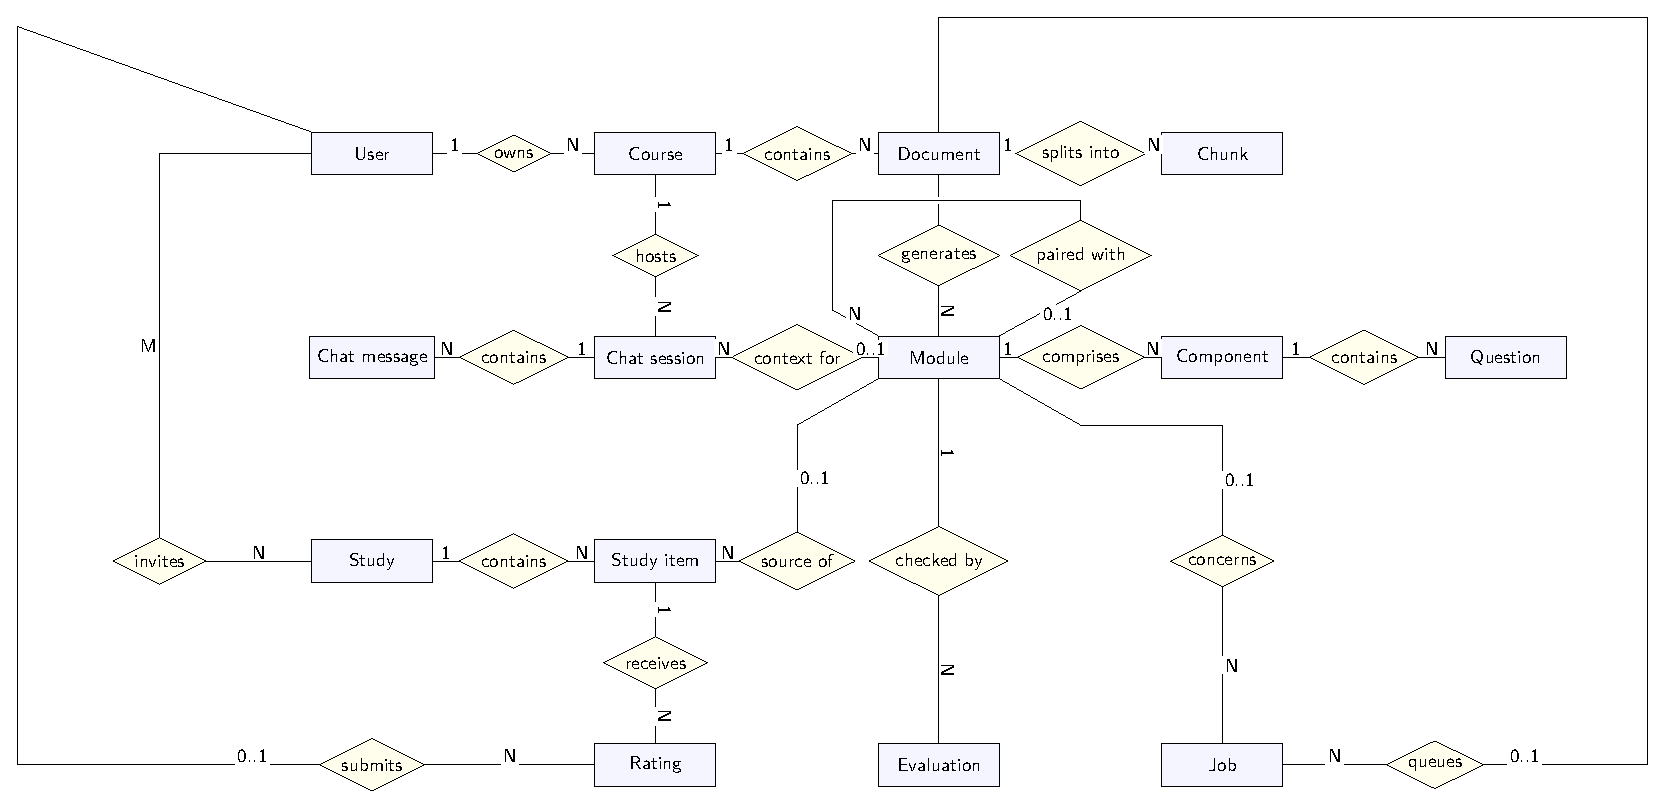
\includegraphics[width=\linewidth,height=.82\textheight,keepaspectratio]{diagrams/erd-overview.pdf}
\caption{Complete Chen overview: entities and relationships without attributes. M and N denote independently varying many sides (including zero); 1 denotes exactly one; 0..1 denotes an optional single entity.}
\label{fig:erd-overview}
\end{figure}
\end{landscape}
\diagram{erd-core}{Chen ERD for the authoring core, with selected attributes and one-to-many relationships.}{erd-core}
\diagram{erd-study}{Chen ERD for research snapshots and ratings. Invitation is a conceptual many-to-many relationship stored as an email list; dashed entities reference the authoring core.}{erd-study}
\diagram{erd-operations}{Chen ERD for operational jobs, conversation history and pipeline evaluations. Dashed entities reference the authoring core; optional module links are specified in the mapping table.}{erd-ops}
\needspace{10\baselineskip}
\subsection{Core relational mapping}
\par
Table~\ref{tab:schema} presents core entity-to-table mapping.
\begin{longtable}{|p{2.8cm}|p{7.0cm}|p{4.1cm}|}\caption{Core entity-to-table mapping.}\label{tab:schema}\\\hline
Table & Important columns and keys & Purpose / invariant\\\hline\endfirsthead
\hline Table & Important columns and keys & Purpose / invariant\\\hline\endhead
\code{users} & universally unique identifier (UUID) primary key (PK); unique email; password hash; active/admin flags; optional unique Moodle user ID; model preference & Local identity independent of Moodle confirmation\\\hline
\code{courses} & UUID PK; owner foreign key (FK) to users; name; nullable Moodle course ID & Owned authoring workspace; remote target may be shared by multiple app courses\\\hline
\code{documents} & UUID PK; course FK; filename; status; raw text; planner cache & Document processing and concept planning\\\hline
\code{chunks} & UUID PK; document/course FKs; ordered chunk index; content; source reference; vector(768) & Evidence unit and retrievable passage\\\hline
\code{modules} & UUID PK; document/course FKs; title; LO; Bloom level; sub-objectives; generation payload/models; optional paired-module FK & Saved module and experimental pairing\\\hline
\code{module_components} & UUID PK; module FK; type; JSONB content; unique (module, type) & One row per non-LO component type\\\hline
\code{questions} & UUID PK; component FK; stem; choices JSONB; answer key; explanation; position & Editable and exportable quiz/practice questions\\\hline\end{longtable}
The vector dimension is a single 768-dimensional configuration constant shared by embedding and storage. Source locators are serialized text; component content uses PostgreSQL's binary JSON representation (JSONB) for structured fields and Markdown. LO fields belong to \code{modules}, so seven pedagogical parts correspond to six component enum values plus the module's LO fields.

The denormalized \code{course_id} on chunks and modules supports inexpensive scope filters and RLS. A composite foreign key to \code{documents(id, course_id)} prevents these rows from claiming a different course from their source document. Unique component types prevent two competing Content or Quiz rows for one module. Explicit chunk and question positions avoid relying on equal creation timestamps for ordering. These constraints preserve source scope and ordering while JSONB stores the variable structures of generated components.
\subsection{Operational and research mapping}
\par
Table~\ref{tab:05-data-2} presents operational and research entities.
\begin{longtable}{|p{3.0cm}|p{6.6cm}|p{4.3cm}|}\caption{Operational and research entities.}\label{tab:05-data-2}\\\hline
Table & Key fields and links & Behavior\\\hline\endfirsthead
\hline Table & Key fields and links & Behavior\\\hline\endhead
\code{jobs} & Type, document/module references, step, status, payload, attempts, due time and lock metadata & PostgreSQL-backed processing queue; nullable links depend on job type\\\hline
\code{evaluations} & Module FK, criterion, numeric score and notes & Pipeline checks; not formal blind ratings\\\hline
\code{chat_sessions} & Course FK and optional module FK & Course Q\&A or module-specific editing context\\\hline
\code{chat_messages} & Session FK, role, text, citations and applied-edit flag & Persisted conversation and edit evidence\\\hline
\code{refresh_tokens} & User FK, unique token hash, expiry and revocation & Server-side session renewal control\\\hline
\code{studies} & Name, rubric version, status and JSONB invited email list & Draft/active/closed study organization\\\hline
\code{study_items} & Study FK, anonymous code, group, nullable source module FK and JSONB packet & Frozen blinded material; group hidden from raters\\\hline
\code{ratings} & Item FK, nullable user FK, rater kind, eight score/reason objects and notes & Human rating or LLM-judge slot, separate from pipeline checks\\\hline\end{longtable}
A RAG study item has exactly one referenced module; a human or LLM-only item is a self-contained packet without that source FK. A source module can have snapshots in different studies, with at most one per study. Human ratings belong to one user and item. LLM-judge ratings have no user ID; the partial unique index allows one LLM-judge rating per item. The conceptual User--Study invitation is physically an email list in \code{studies}, not a junction table. Blinded views enforce what a rater can read.

Study source and rater foreign keys use \code{RESTRICT} where necessary to preserve provenance. A source edit does not mutate its snapshot. Deleting a referenced module, document or course must first address its research dependencies and returns a conflict rather than silently discarding the snapshot. A two-judge experiment stores separate result packets keyed by judge model and packet hash.
\subsection{Citation and edit representation}
The citation model stores a server-created \code{source_map} from codes such as S1 to physical chunk ID and locator. It derives \code{inline_citations} from saved Markdown, including claim and marker character offsets. These are offsets in the saved string, not PDF coordinates or byte offsets. Adjacent markers can share a claim span. Invalid or malformed source codes are rejected; span-validation scenarios include abbreviations, mathematics and complex Markdown.

An \code{ai_original} object in component JSON preserves the pre-edit version on the first modification. For question-bearing components, it also includes ordered question fields. The edit operation preserves corresponding explanation data when a question explanation changes. The original snapshot remains unchanged after subsequent edits. For experiments, a frozen unedited module/packet remains the preferred analysis artifact.

\clearpage\section{Document, retrieval and generation pipelines}
\subsection{Ingestion: read, chunk and embed}
The author uploads a file into an owned course. The API validates format and streamed size, stores the binary under a generated identifier, and creates a document/job record. The background worker executes extraction, chunking and embedding as durable steps. It removes the temporary file after successful processing.
Figure~\ref{fig:ingestion} shows proposed asynchronous ingestion and bounded error recovery.
\diagram{ingestion}{Proposed asynchronous ingestion and bounded error recovery.}{ingestion}
\subsubsection{Readers and source locators}
PDF uses PyMuPDF with layout/font rules and OCR for low-text pages. PowerPoint extraction retains slide text and speaker notes. Narrative and transcript readers provide the same document-unit interface. Each unit carries text and a page, slide or timestamp locator. Source-quality checks identify empty pages, suspicious extraction and omitted visual content for instructor review.
\subsubsection{Chunking and embedding}\label{sec:chunking}
The chunker follows source structure before applying size limits. PDF and presentation readers supply page/slide units with physical locators. Short units can share a chunk, but no chunk spans more than two distinct pages or slides; the combined content is checked before merging. A long unit uses word-boundary windows and keeps the same page/slide locator with a part index. Timestamped captions are accumulated as transcript segments, retaining their minimum start and maximum end time. Oversized individual captions are split without overlap; accumulation stops after crossing its target, so 150 is a soft target rather than a strict maximum.

Narrative DOCX, HTML and plain text use recursive splitting: blank-line boundary, newline, period followed by space, space, then character fallback. This extends LangChain's recursive-separator approach with a sentence separator and a custom length function\citep{recursivesplit}. The estimator counts each Unicode word as one plus its length divided by seven (rounded down), then adds one for every non-word, non-whitespace symbol. It is a lightweight estimate, not the embedding model's tokenizer. Source-unit positions and headings are retained when a narrative chunk crosses a boundary.

Table~\ref{tab:chunk-parameters} gives the canonical settings. The filename supplies a readable title; a nonredundant section or slide heading is prefixed after content splitting. Token estimates are then recomputed, so the content cap does not include this prefix. At generation time, up to two neighboring physical chunks on either side supply context; they keep separate source IDs and citations.
\begin{table}[H]\centering\small\caption{Structure-aware chunking and generation-context parameters.}\label{tab:chunk-parameters}
\begin{tabularx}{\linewidth}{|p{4.3cm}|p{2.1cm}|Y|}\hline
Parameter & Value & Meaning\\\hline
Content budget & 340 & Estimated tokens before title/heading prefix\\\hline
Narrative overlap & 50 & Estimated-token overlap in recursive splitting\\\hline
Page/slide grouping & Target 250; at most 2 & Flush at target; at most two distinct pages/slides; check 340 before merging\\\hline
Long-page overlap & 40 & Word-boundary split of oversized page/slide units\\\hline
Transcript target & 150 & Timestamp accumulation target; long captions split with zero overlap\\\hline
Context prefix & Title + heading & Omit redundant heading; recompute estimated length\\\hline
Generation neighbors & $\pm 2$ & Same-document physical neighbors retain individual source codes\\\hline
\end{tabularx}\end{table}
The 340-token content budget reserves room for a query and prefix against the 512-token BGE comparison service; the selected Qwen3/Jina services accept 1,024 model tokens. Estimated and model-token lengths differ, so truncation must still be checked. Smaller page/transcript targets support precise citation locators. Fixed-size splitting is simple but can sever code or topic boundaries; semantic splitting adds embedding-based boundary computation. Qu et al. find no consistent gain that justifies its cost across their tasks\citep{semanticchunking}. The design therefore retains structure-aware/recursive splitting and compares alternatives on held-out material, rather than assuming semantic splitting is superior.

The gateway's \code{embed-default} alias routes embedding to local Qwen3-Embedding-0.6B. Queries use the instructed retrieval prefix; document text does not. The 768-dimensional normalized representation uses a common revision\citep{qwen}; changing it requires consistent corpus re-embedding and cache refresh.
\subsection{Retrieval}
\subsubsection{Scope, candidates and ranking}\label{sec:retrieval-policy}
Module queries are filtered by the authorized course and selected document; course Q\&A uses the authorized course as its boundary. Dense cosine search and BM25 each return ranked candidates; RRF combines their positions with damping constant 60\citep{bm25,rrf}. A scoped BM25 cache stores chunk IDs and is invalidated after ingestion or deletion.

Jina multilingual INT8 reranks up to 30 candidates. LO and Content use adaptive-$k$ with floor eight. Practice/Quiz retrieval for each sub-objective uses fixed $k=4$. Module-edit chat uses fixed $k=8$, while course Q\&A uses fixed $k=5$. Adaptive selection finds the largest adjacent gap within the leading 90\%, adds five and enforces floor eight\citep{adaptive}. A flat score distribution retains the search window. Dense bypass provides a fallback when reranking is unavailable.
\subsubsection{Physical evidence and corrective retrieval}
Neighbor expansion supplies up to two physical chunks on either side of a hit. Each passage keeps its own ID and locator and receives a separate source code in the prompt. The saved source map and evaluation packets resolve those same physical units.

The relevance evaluator assesses whether the retrieved set supports the LO and sub-objectives. If confidence is low, it proposes one refined query, merges the new passages by identity and reassesses\citep{correctiverag}. The result stores confidence and retry count for the generation record.
\subsection{Generation orchestration}\label{sec:generation}
Figure~\ref{fig:generation} shows retrieval and generation flow with physical inline citations.
\diagram{retrieval-generation}{Retrieval and generation flow with physical inline citations.}{generation}
\subsubsection{Planner and learning objectives}
The planner extracts up to eight ranked concepts from the first 8,000 characters of document text. Its result is cached per document. Each generation request selects one priority concept and retrieves broad evidence to derive a terminal LO, Bloom level and enabling sub-objectives.

For broad documents, the planner budget bounds cost. Phase 2 will assess concept coverage, including topics occurring beyond the prefix, and compare the selected objective with instructor expectations.
\subsubsection{Content and inline citations}
Content follows the LO and uses one heading per sub-objective. The prompt supplies physical passages with server-assigned codes. Important statements carry adjacent Markdown markers, for example \code{Heap insertion takes O(log n). [S2]}.

The server validates marker membership and derives claim/marker character spans from the saved text. It resolves the chunk ID and page/slide/timestamp through the source map. Unknown markers are rejected. When several passages jointly support a statement, adjacent markers share the claim span. The source panel displays the corresponding text beside the lesson for instructor inspection.
\needspace{.55\textheight}
\subsubsection{Grounding and pedagogical freedom}\label{sec:grounding-policy}
Table~\ref{tab:grounding-policy} separates source-required knowledge from permitted instructional invention. This policy controls generation and defines the denominator of the source-support assessment.
\begin{table}[H]\centering\small\caption{Grounding policy for generated teaching material.}\label{tab:grounding-policy}
\begin{tabularx}{\linewidth}{|p{3.0cm}|Y|}\hline
Part & Grounding rule\\\hline
Lesson content & Facts, definitions and formulas come from supplied passages with \code{[S\#]} citations. The model may paraphrase and connect ideas, but adds no new knowledge.\\\hline
Illustrative examples & Worked examples and code may be created, labelled ``Illustrative example,'' and consistent with source concepts. Code is checked by execution in an isolated environment where possible.\\\hline
Practice and Quiz & New scenarios may elicit Apply/Analyze processes. Correct answers must be derivable from cited sources. Distractors may express model-generated common misconceptions and need no citation; each explanation cites the passage supporting the correct answer.\\\hline
Source gaps & Missing knowledge required by an objective is flagged to the lecturer instead of supplied from model knowledge.\\\hline
Support assessment & Assess source-required facts, correct answers and explanations. Exclude explicitly illustrative material and distractors from the support denominator.\\\hline
\end{tabularx}\end{table}
The permitted invention supplies a setting for learners to use a concept rather than introducing unsupported lesson knowledge. The instructor reviews scenario validity, misconception plausibility and the stated Bloom demand. A failed or unavailable code execution check is recorded and surfaced for review, rather than interpreted as success. Source support and pedagogical quality remain separate acceptance dimensions: a configuration that repeats only easy factual questions cannot win solely by achieving a high support score. The question-generation literature motivates evaluating difficulty and feedback alongside factual acceptability\citep{aqgreview}.
\subsubsection{Slides, example, questions and explanation}
Slides and examples are generated as structured objects aligned with the Content and LO. Practice and Quiz retrieve narrower evidence for each objective. A bounded question-generation loop validates stems, choices, correct-answer indices and explanations. Learner-facing fields use the selected English or Vietnamese output language; quoted source material keeps its language.

Ordered Question rows store editable fields, while the Explanation component links reasoning to question type and position. A manual or chat edit updates the question and corresponding explanation together. The first edit saves an immutable \code{ai_original} snapshot; subsequent edits update the teaching version and retain that original.
\subsubsection{Self-check and comparison condition}
The Content critic checks completeness, scope and source support. Practice/Quiz checks evaluate answerability and, in the RAG condition, groundedness. Bounded regeneration limits time and token consumption. Structured validation and unknown-citation checks are enforced before storage; semantic check results remain part of the module record.

The LLM-only comparison follows the matched source-withholding condition in Section~\ref{sec:conditions}. Comparison modules remain research material and cannot be published through the Moodle endpoint.
\subsection{Gateway routing and model control}
The LiteLLM gateway centralizes provider keys, model aliases, structured output and retry policy\citep{litellm}. Normal use can route eligible small steps to a lower-cost backup and fall back after transient failures. Content uses the selected generation profile.

Table~\ref{tab:model-aliases} names the generation profiles once. Experiment mode disables cross-model fallback; each output records the requested profile, served model, prompt version and settings. Local Qwen3 embedding remains constant across generation conditions.
\begin{table}[H]\centering\small\caption{Generation model profiles and gateway aliases.}\label{tab:model-aliases}
\begin{tabularx}{\linewidth}{|p{3.1cm}|p{4.1cm}|Y|}\hline
Alias & Model & Role\\\hline
\code{claude-fast} & Claude Haiku 5.5 & Paid primary comparison candidate\\\hline
\code{openai-fast} & GPT-6 Luna & Paid primary comparison candidate\\\hline
\code{claude-pro} & Claude Sonnet 5.5 & Higher-tier bounded comparison\\\hline
\code{openai-pro} & GPT-6.1 Sol & Higher-tier bounded comparison\\\hline
\end{tabularx}\end{table}

\clearpage\section{Moodle integration and security}\label{sec:security}
\subsection{Identity linking and course authority}
The integration boundary consists of Moodle Web Services\citep{moodlews} and the \code{local_lms_bridge} plugin. The bridge provides identity, capability and publication contracts.

Local application identity and Moodle identity are independent. Registration does not prove control of a Moodle account. A link request produces an opaque request ID; a matching Moodle user must sign in and confirm on the Moodle side. The application then stores the confirmed Moodle user ID. A generic pending response prevents the link-request response from revealing whether the entered email matches an active account. Missing and ambiguous emails receive pending requests with the same externally visible shape; only legitimate confirmation may reveal identity.

A confirmed identity does not automatically grant access to every Moodle course. The bridge queries course authoring capabilities and verifies the requested actor in the course context. The author ID is propagated on creation calls. The bridge also checks relevant activity/question capabilities in its external handlers. The application administrator is not treated as a Moodle administrator solely because the local admin flag is true. Rights can be revoked externally, so publication verifies them immediately before activity writes.
\subsection{Publication mapping and sequence}
The Book receives navigable lesson material, including the LO and usable generated content. Practice is published as a quiz with immediate feedback; the assessment Quiz uses deferred feedback. Question stems, choices and explanations are exported from the live saved question data. The target section is chosen by the author. Moodle's Book and Quiz remain the actual learner-facing activities\citep{moodlebook,moodlequiz}.
Figure~\ref{fig:moodle} shows publication sequence and permission checks. Book and subsequent quiz writes are separate remote operations.
\diagram{moodle-sequence}{Publication sequence and permission checks. Book and subsequent quiz writes are separate remote operations.}{moodle}
The application sanitizes HTML through an allowlist before transmission and returns created activity IDs. Book, Practice and Quiz are separate remote operations. If a later operation fails, earlier activities can remain. The publication design records external IDs and per-step state, expose partial success and support safe resumption during recovery.
\subsection{Authentication and session security}
Passwords are stored as bcrypt hashes\citep{bcrypt}. The password path guards bcrypt's byte-length boundary. JSON Web Token (JWT) access tokens\citep{jwt} require subject and expiry and are decoded using the configured algorithm. Token claims identify the user, while active/admin state is read from the database. Refresh tokens are high-entropy opaque values stored by SHA-256 hash with expiry and revocation state; refresh rotates them. The browser keeps a short-lived access token in memory; its design lifetime is 15 minutes. The rotating refresh token uses a Secure, HttpOnly, SameSite cookie scoped to the refresh endpoint, so scripts cannot read it. Origin checks and a cross-site request forgery (CSRF) token protect cookie-authenticated renewal. Markdown/HTML sanitization and a restrictive content security policy (CSP) reduce cross-site scripting (XSS) exposure; cookie protection does not make injected scripts harmless.

Logout revokes the presented refresh token and clears client state. An already issued access token remains subject to its expiry and the active-account check; access-token expiration is enforced on each request. Disabling a user blocks protected requests through the authenticated-user dependency. Production settings reject weak/default secrets and separate owner, runtime and worker database credentials.
\subsection{Row-level security and ownership}
The Open Worldwide Application Security Project (OWASP) emphasizes server-side ownership and deny-by-default authorization\citep{owaspaccess}. The application uses both ownership checks and PostgreSQL row-level security (RLS). PostgreSQL documents that table owners and privileged roles normally bypass row policies\citep{postgresrls}; consequently, request sessions use a restricted runtime role rather than a superuser.

The runtime role is distinct from the schema owner. A validated user identity is set as transaction-local database context and reapplied at the start of every transaction. Course-owned content is filtered by policies. The worker has a separate role with the cross-owner visibility needed to process jobs and restricted grants; it is a trusted service boundary, not a user session.

Blind study views omit group/source identifiers as well as filtering rows. Ordinary RLS filters rows but cannot alone hide selected columns from a response. Ratings policies allow invited users to read/write only their own human ratings; removal of an invitation removes that access while preserving the historical rating for the study owner. Administrative job retry uses a narrow database function rather than giving the admin general access to every course's content.
\subsection{Indirect prompt-injection checks}\label{sec:prompt-injection}
Uploaded course material is untrusted model input. The ingestion design scans extracted text for instruction-like patterns, role impersonation, requests to ignore constraints and attempts to solicit credentials or external actions. Suspicious passages are flagged with their locators for lecturer inspection; legitimate code or security teaching examples may resemble attacks, so a flag is evidence for review rather than proof of malice. OWASP identifies such indirect instructions as a distinct prompt-injection path\citep{owaspprompt}.

Prompt construction keeps system instructions separate from source data and labels every retrieved passage with its source identity and trust level. Spotlighting applies a continuous provenance signal, including datamarking, to help the model distinguish untrusted text from instructions\citep{spotlighting}. Marking changes only the prompt representation: original source text and physical locators remain intact for citation inspection. It supplements explicit source delimiters and the instruction to treat source passages as data.

Before saving, the server validates output schemas, answer indices and citation membership. The model never decides authorization, grants access or initiates Moodle publication; authenticated API checks and database policies enforce those boundaries independently. Phase 2 will run an adversarial-document suite with benign controls, hidden/encoded instructions, multilingual role imitation and attempted citation or content contamination. It records attack success, false-positive flags, grounded task quality and validation failures, and asserts that no generated text bypasses ownership or capability checks. Prompt marking is tested as a risk-reduction measure, not assumed to be a complete security boundary.
\subsection{Threats, controls and verification targets}
The security design maps trust boundaries to controls and Phase 2 verification scenarios.
\par
Table~\ref{tab:07-moodle-security-1} presents security controls and their limits.
\begin{longtable}{|p{3.0cm}|p{5.8cm}|p{5.1cm}|}\caption{Security controls and their limits.}\label{tab:07-moodle-security-1}\\\hline
Threat & Proposed control & Phase 2 verification\\\hline\endfirsthead
\hline Threat & Proposed control & Phase 2 verification\\\hline\endhead
Cross-owner object access & Ownership checks, course/document filters, composite FKs and RLS; uniform missing-resource response & Direct API and runtime-role DB probes across owners and after transaction restart\\\hline
Account enumeration & Generic Moodle pending link response & Equivalent status and expiry for matching, missing and ambiguous emails; transport errors remain distinct\\\hline
Unsafe rendered content & Moodle HTML allowlist; structured model output & Markdown preview and exported activity XSS cases, including source text\\\hline
Resource exhaustion & Streamed upload limits, JSON body limit, route limits and daily generation cap for untrusted accounts & Concurrent uploads/jobs, provider quota exhaustion, CPU/RAM and fair scheduling\\\hline
Indirect prompt injection & Document scanning/lecturer flags, prompt-only datamarking, separated instructions and output validation (Section~\ref{sec:prompt-injection}) & Adversarial source tests; prompting alone is not a security boundary\\\hline
Credential exposure & Provider keys stay at gateway; separate DB roles; secret-aware configuration fields & Production configuration, logs, rotation and backup access\\\hline
Publication misuse & Confirmed actor plus fresh Moodle capability checks & Unlinked, revoked, suspended and wrong-course scenarios\\\hline
Blinding failure & Restricted views, own-rating policies and snapshots & Response field audit and packet-text leakage review\\\hline
\end{longtable}
OWASP's generative-AI guidance identifies external content as an injection path\citep{owaspprompt}. The LLM does not decide authorization or receive unrestricted database tools. Provider-generated output remains untrusted input to schema validation and renderer sanitization.

Request middleware limits ordinary JSON bodies and supplies security headers. Uploads are exempt from that generic body limit but have their own streamed limits. Upload limits are 50 MB for ordinary documents, 200 MB for audio and 500 MB for video. Production hides API documentation and adds transport/content-security headers. External LLM calls transmit selected source text; local embedding runs on the application host. Before public use, provider disclosures, data retention and consent must be specified for the actual deployment.

\clearpage\section{API design summary}\label{sec:api}
\subsection{Resource and asynchronous contracts}
The application programming interface (API) uses FastAPI and JavaScript Object Notation (JSON) resources with local UUIDs; uploads use multipart data and PPTX export returns binary content. Moodle IDs remain remote identifiers. OpenAPI is exposed in development and disabled publicly in production. Upload and generation responses identify durable jobs for polling. Identity-link requests return an opaque pending request, with confirmation checked through a separate state resource.
\par
Table~\ref{tab:08-api-1} presents representative endpoint groups; resource contracts and authorization.
\begin{longtable}{|p{6.6cm}|p{7.3cm}|}\caption{Representative endpoint groups; resource contracts and authorization.}\label{tab:08-api-1}\\\hline
Method / resource & Contract and authorization\\\hline\endfirsthead
\hline Method / resource & Contract and authorization\\\hline\endhead
\code{POST /auth/register}, \code{/auth/login}, \code{/auth/refresh}, \code{/auth/logout} & Validate credentials; issue, renew or revoke the session\\\hline
\code{GET, POST /courses}; \code{DELETE /courses/{id}} & Owned workspaces; deletion conflicts with protected study sources\\\hline
\code{GET /courses/moodle/courses}; \code{POST /courses/{id}/link-moodle} & Confirmed identity and remote course-author rights\\\hline
\code{POST /documents}; \code{GET /documents?course_id=...}; \code{GET /documents/jobs/{job_id}} & Upload/list owned source and poll processing\\\hline
\code{POST /modules/generate}; \code{GET /modules/jobs/{job_id}} & Freeze source/model/language/guidance settings; poll to a saved module ID\\\hline
\code{GET, PATCH /modules/{id}}; \code{PATCH /modules/{id}/components/{cid}}; \code{PATCH /modules/{id}/questions/{qid}} & Owner reads/edits; original retention, citation validation and synchronized explanations\\\hline
\code{POST /modules/{id}/chat-edit}; \code{GET /modules/{id}/slides.pptx} & Authorized structured AI edit or current Slides download\\\hline
\code{POST /modules/{id}/publish-to-moodle} & Owned RAG module, confirmed actor and authorized target\\\hline
\code{POST /moodle/account/link-requests}; \code{GET, DELETE /moodle/account} & Generic pending identity request, poll confirmed state or unlink\\\hline
\code{POST /courses/{id}/chat}; \code{GET /courses/{id}/chat/{session}/history} & Owner-only course Q\&A, source citations and conversation history\\\hline
\code{GET /models}; \code{PUT /models/default} & Available aliases and user preference\\\hline
\code{POST /jobs/{id}/retry}; \code{GET /admin/jobs/failed}; \code{POST /admin/jobs/retry} & Own-job recovery or narrow admin recovery scope\\\hline
\code{GET /admin/users} and account actions & Administrator-only account management\\\hline
\code{POST, GET /studies}; \code{POST /studies/{id}/items}; \code{PUT /studies/{id}/raters} & Admin prepares paired snapshots and invitations\\\hline
\code{GET /studies/mine}; \code{GET /studies/mine/{id}/items}; \code{PUT /studies/mine/{id}/items/{item}/rating} & Invited rater reads blinded packets and writes own rating only\\\hline\end{longtable}
\subsection{Validation and client state}
Authentication failures normally return 401; missing/non-owned resources use 404. Validation uses 422, oversized uploads 413, protected/concurrent-state conflicts 409 and rate limits 429. Catalog unavailability maps to 503 without revealing its internal URL. Moodle helpers distinguish remote identity, capability and service failures.

Clients poll job outcomes after submission and open a module only after completion. They distinguish a pending link, confirmed identity and course-specific permission. Source review and saved edits precede export/publication. Generation settings and served-model history belong in researcher manifests; ordinary screens need clear state and actions rather than raw internal fields.

\clearpage\section{UI/UX design}\label{sec:ui}
\subsection{Navigation and interaction principles}
The GENAILMS interface uses Vietnamese microcopy and role-specific views. The authoring flow is dashboard $\rightarrow$ documents $\rightarrow$ generation $\rightarrow$ review/edit $\rightarrow$ publication. Each screen emphasizes one primary action; menus, tooltips and expandable rows hold secondary detail. Citation inspection and AI chat sit beside the lesson, preserving reading context during review. Status combines words, icons and colour.

\par
Table~\ref{tab:09-ui-1} presents interface typography, spacing and accessibility rules.
\begin{table}[H]\centering\small\caption{Interface typography, spacing and accessibility rules.}\label{tab:09-ui-1}
\begin{tabularx}{\linewidth}{|p{3.0cm}|Y|Y|}\hline
Concern & Design rule & Design rationale\\\hline
Readability & IBM Plex Sans body 16/24 px; small 14/20; reading 16/27 & Readable text and Vietnamese diacritics at desktop and mobile sizes\\\hline
Hierarchy & Newsreader page titles 28/36; sans section/dialog headings 20/28 & Distinct page hierarchy with consistent functional headings\\\hline
Control visibility & Input borders \code{\#8F8778}; navy focus ring & Measured contrast 3.56:1 on white, 3.35:1 on cream, 3.12:1 on subtle: above the 3:1 control-border target\citep{wcag}\\\hline
Rhythm & 4/8 spacing scale; 1120 px content cap; text at most 72ch & Consistent alignment and manageable reading length\\\hline
Feedback & Text errors, labelled status, empty/loading/error states and mobile actions & Avoid colour-only meaning and show the next useful action\\\hline
\end{tabularx}\end{table}

Keyboard order, dialog focus, live announcements and task completion are acceptance criteria. Table~\ref{tab:screen-design} relates the interaction surfaces to the use cases and design decisions. Vietnamese microcopy is retained in the figures; the surrounding English gloss identifies the primary action. Focused crops enlarge the controls and evidence needed for each discussion.
\begingroup\small
\begin{longtable}{|p{2.8cm}|p{2.1cm}|p{3.7cm}|p{5.1cm}|}\caption{Screen interactions and design rationale.}\label{tab:screen-design}\\\hline
Screen & UC / FR & Primary action & Key design decision\\\hline\endfirsthead
\hline Screen & UC / FR & Primary action & Key design decision\\\hline\endhead
Access & UC01 / FR01 & Sign in or register & Labelled fields, recoverable validation\\\hline
Courses & UC02--03 / FR02--03 & Open course; upload source & Ownership context and visible processing state\\\hline
Generation & UC04,15 / FR04,15 & Confirm model, language and guidance & Saved preference preselects a per-request choice\\\hline
Source review & UC05 / FR05 & Inspect citation & Claim and original evidence stay adjacent\\\hline
Editing & UC06--07 / FR06--07 & Apply edit; download slides & Review context and saved-state feedback\\\hline
Publication & UC08--09 / FR08--09 & Link account; publish & Destination, capability and partial-result visibility\\\hline
Administration & UC10--12 / FR10--11,13 & Manage accounts, jobs, studies & Narrow role-specific actions\\\hline
Rating & UC13 / FR12 & Score anonymous packet & Stable order, criterion reasons and source access\\\hline
Course Q\&A & UC14 / FR14 & Enter course conversation & Course-scoped history and source citations; workspace entry\\\hline
Mobile / states & UC01--15 & Complete or recover a task & One-column actions; text and icons reinforce colour\\\hline
\end{longtable}\endgroup

\needspace{.42\textheight}
The login form in Figure~\ref{fig:ui-screen-01} makes the credential fields and the primary sign-in action explicit. ``Đăng nhập'' means ``Sign in''; ``Mật khẩu'' means ``Password''.
\begin{figure}[H]\centering
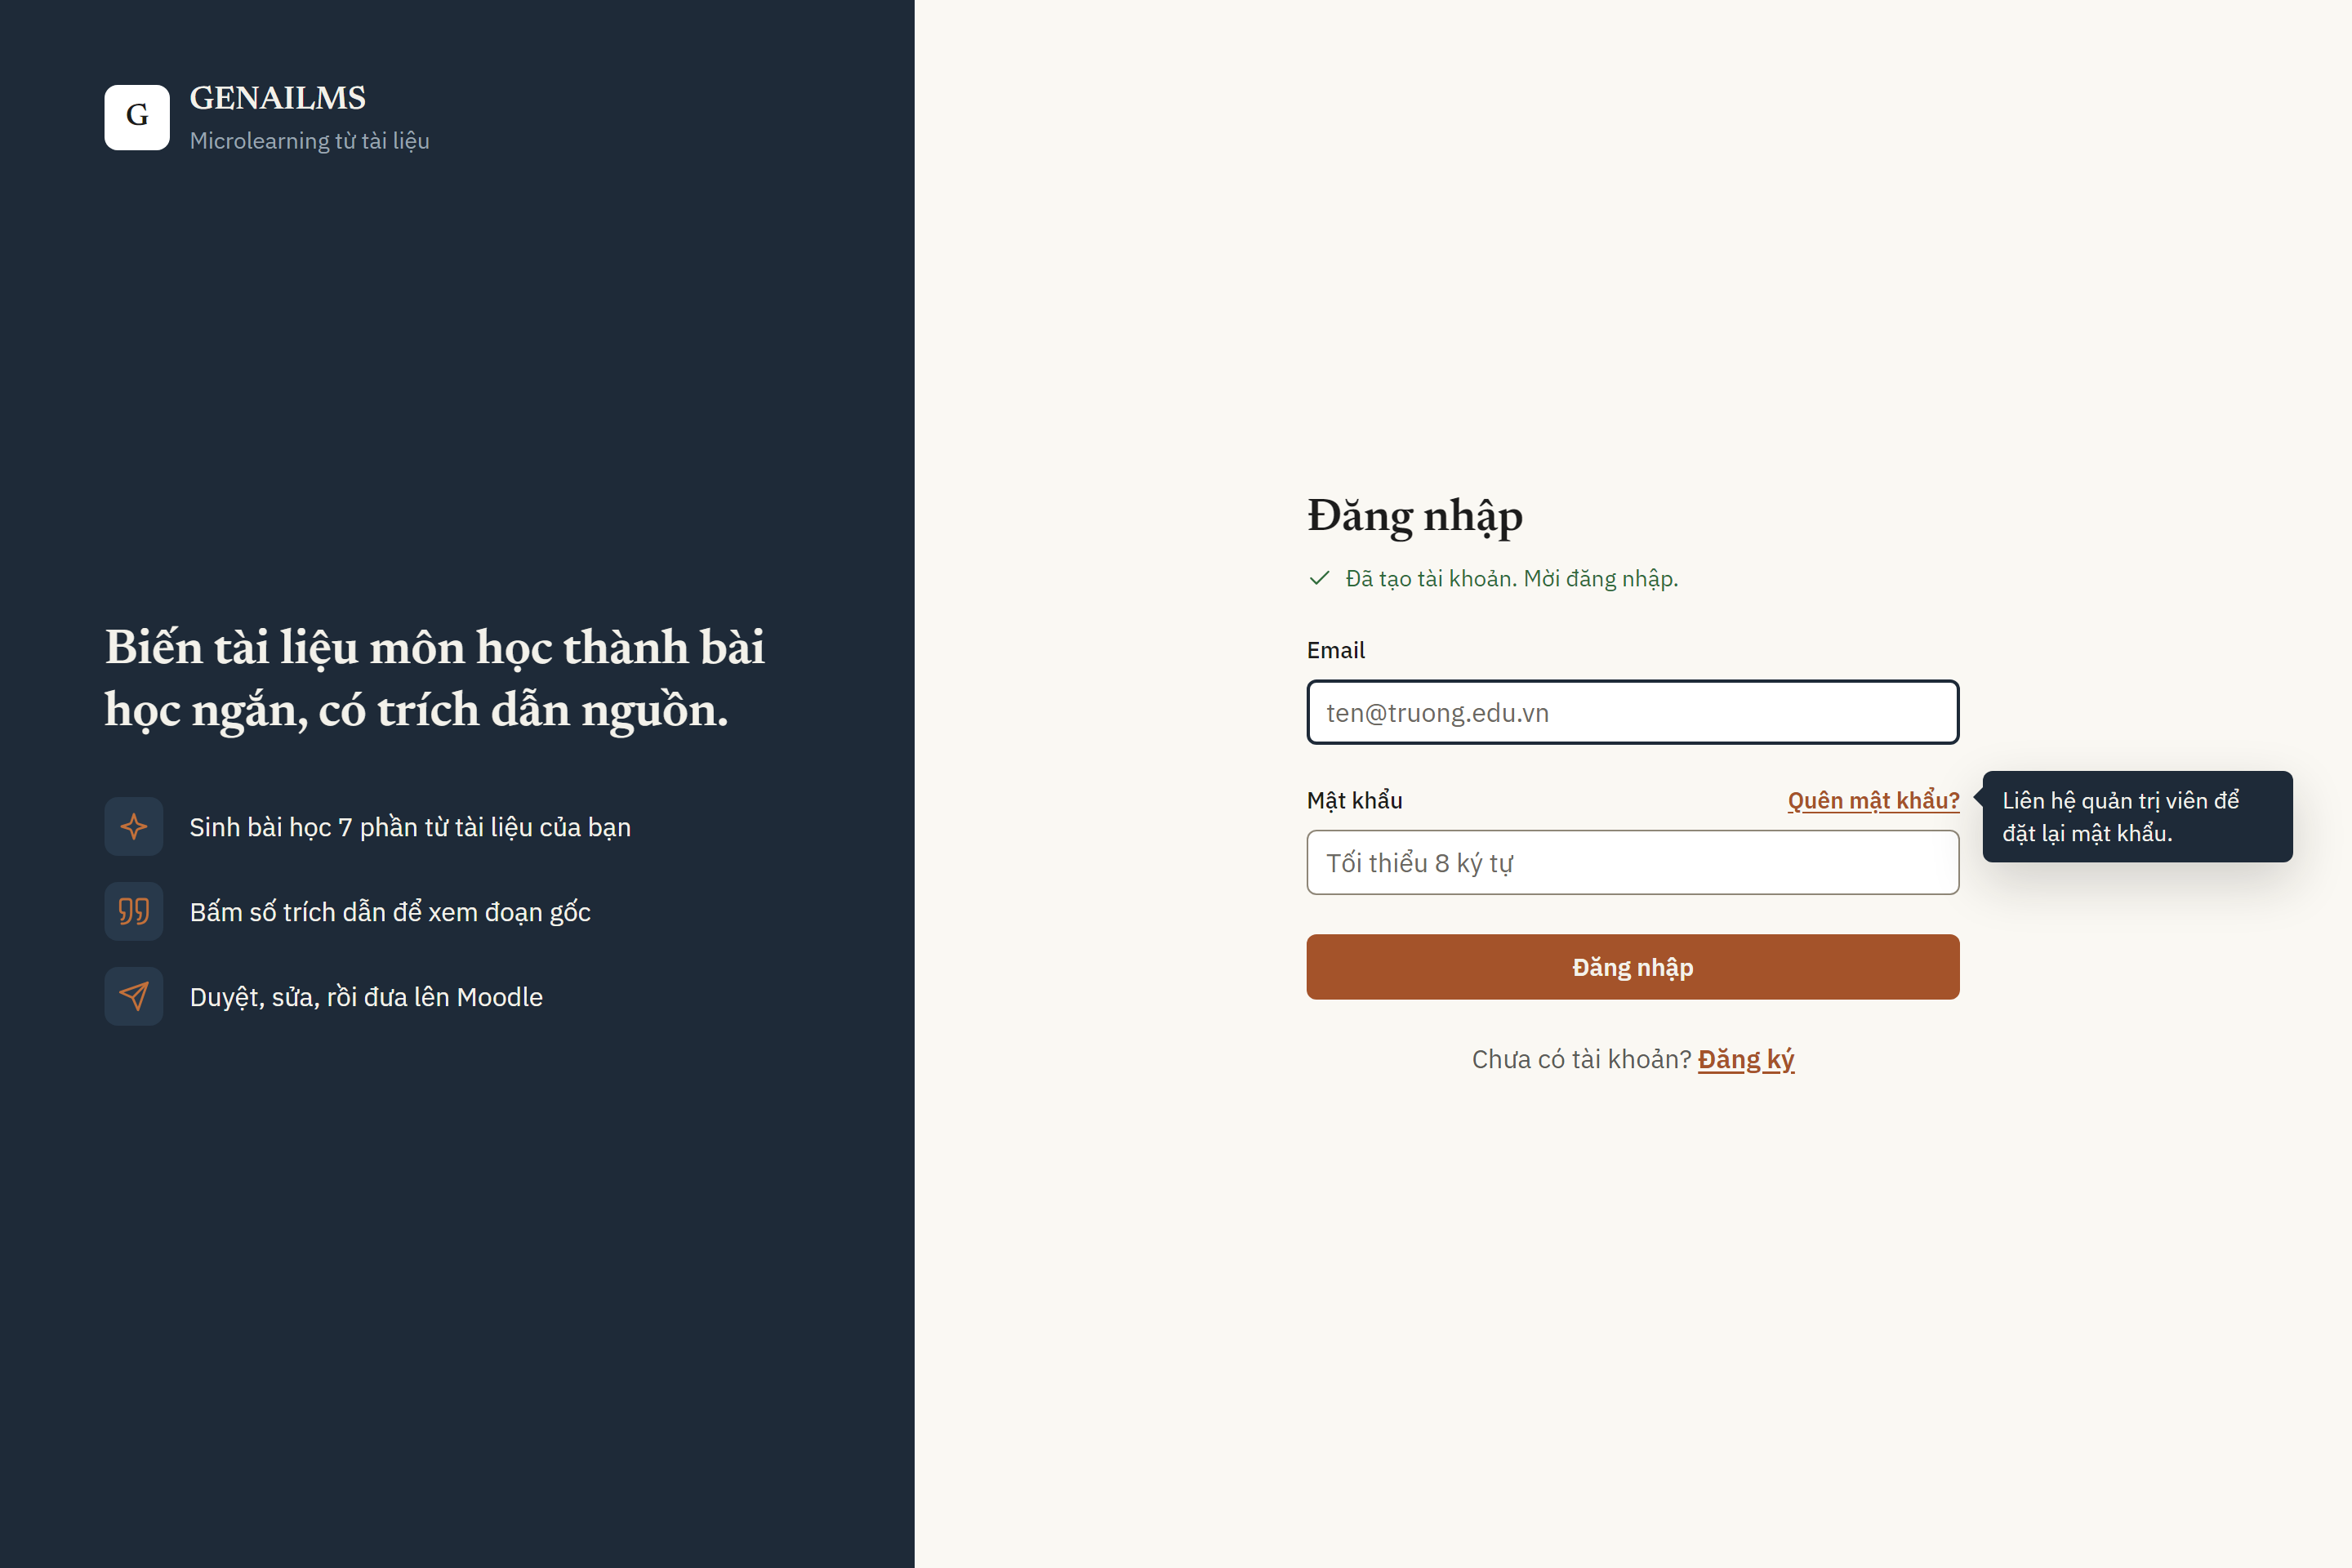
\includegraphics[width=\linewidth,height=.34\textheight,keepaspectratio,viewport={1550 500 2830 1450},clip]{graphics/ui/01-login.png}
\caption{Credential entry and sign-in feedback.}\label{fig:ui-screen-01}
\end{figure}

\needspace{.42\textheight}
Figure~\ref{fig:ui-screen-02} presents registration with persistent labels and repeated-password validation. ``Đăng ký'' means ``Register''; validation remains next to the field that needs correction.
\begin{figure}[H]\centering
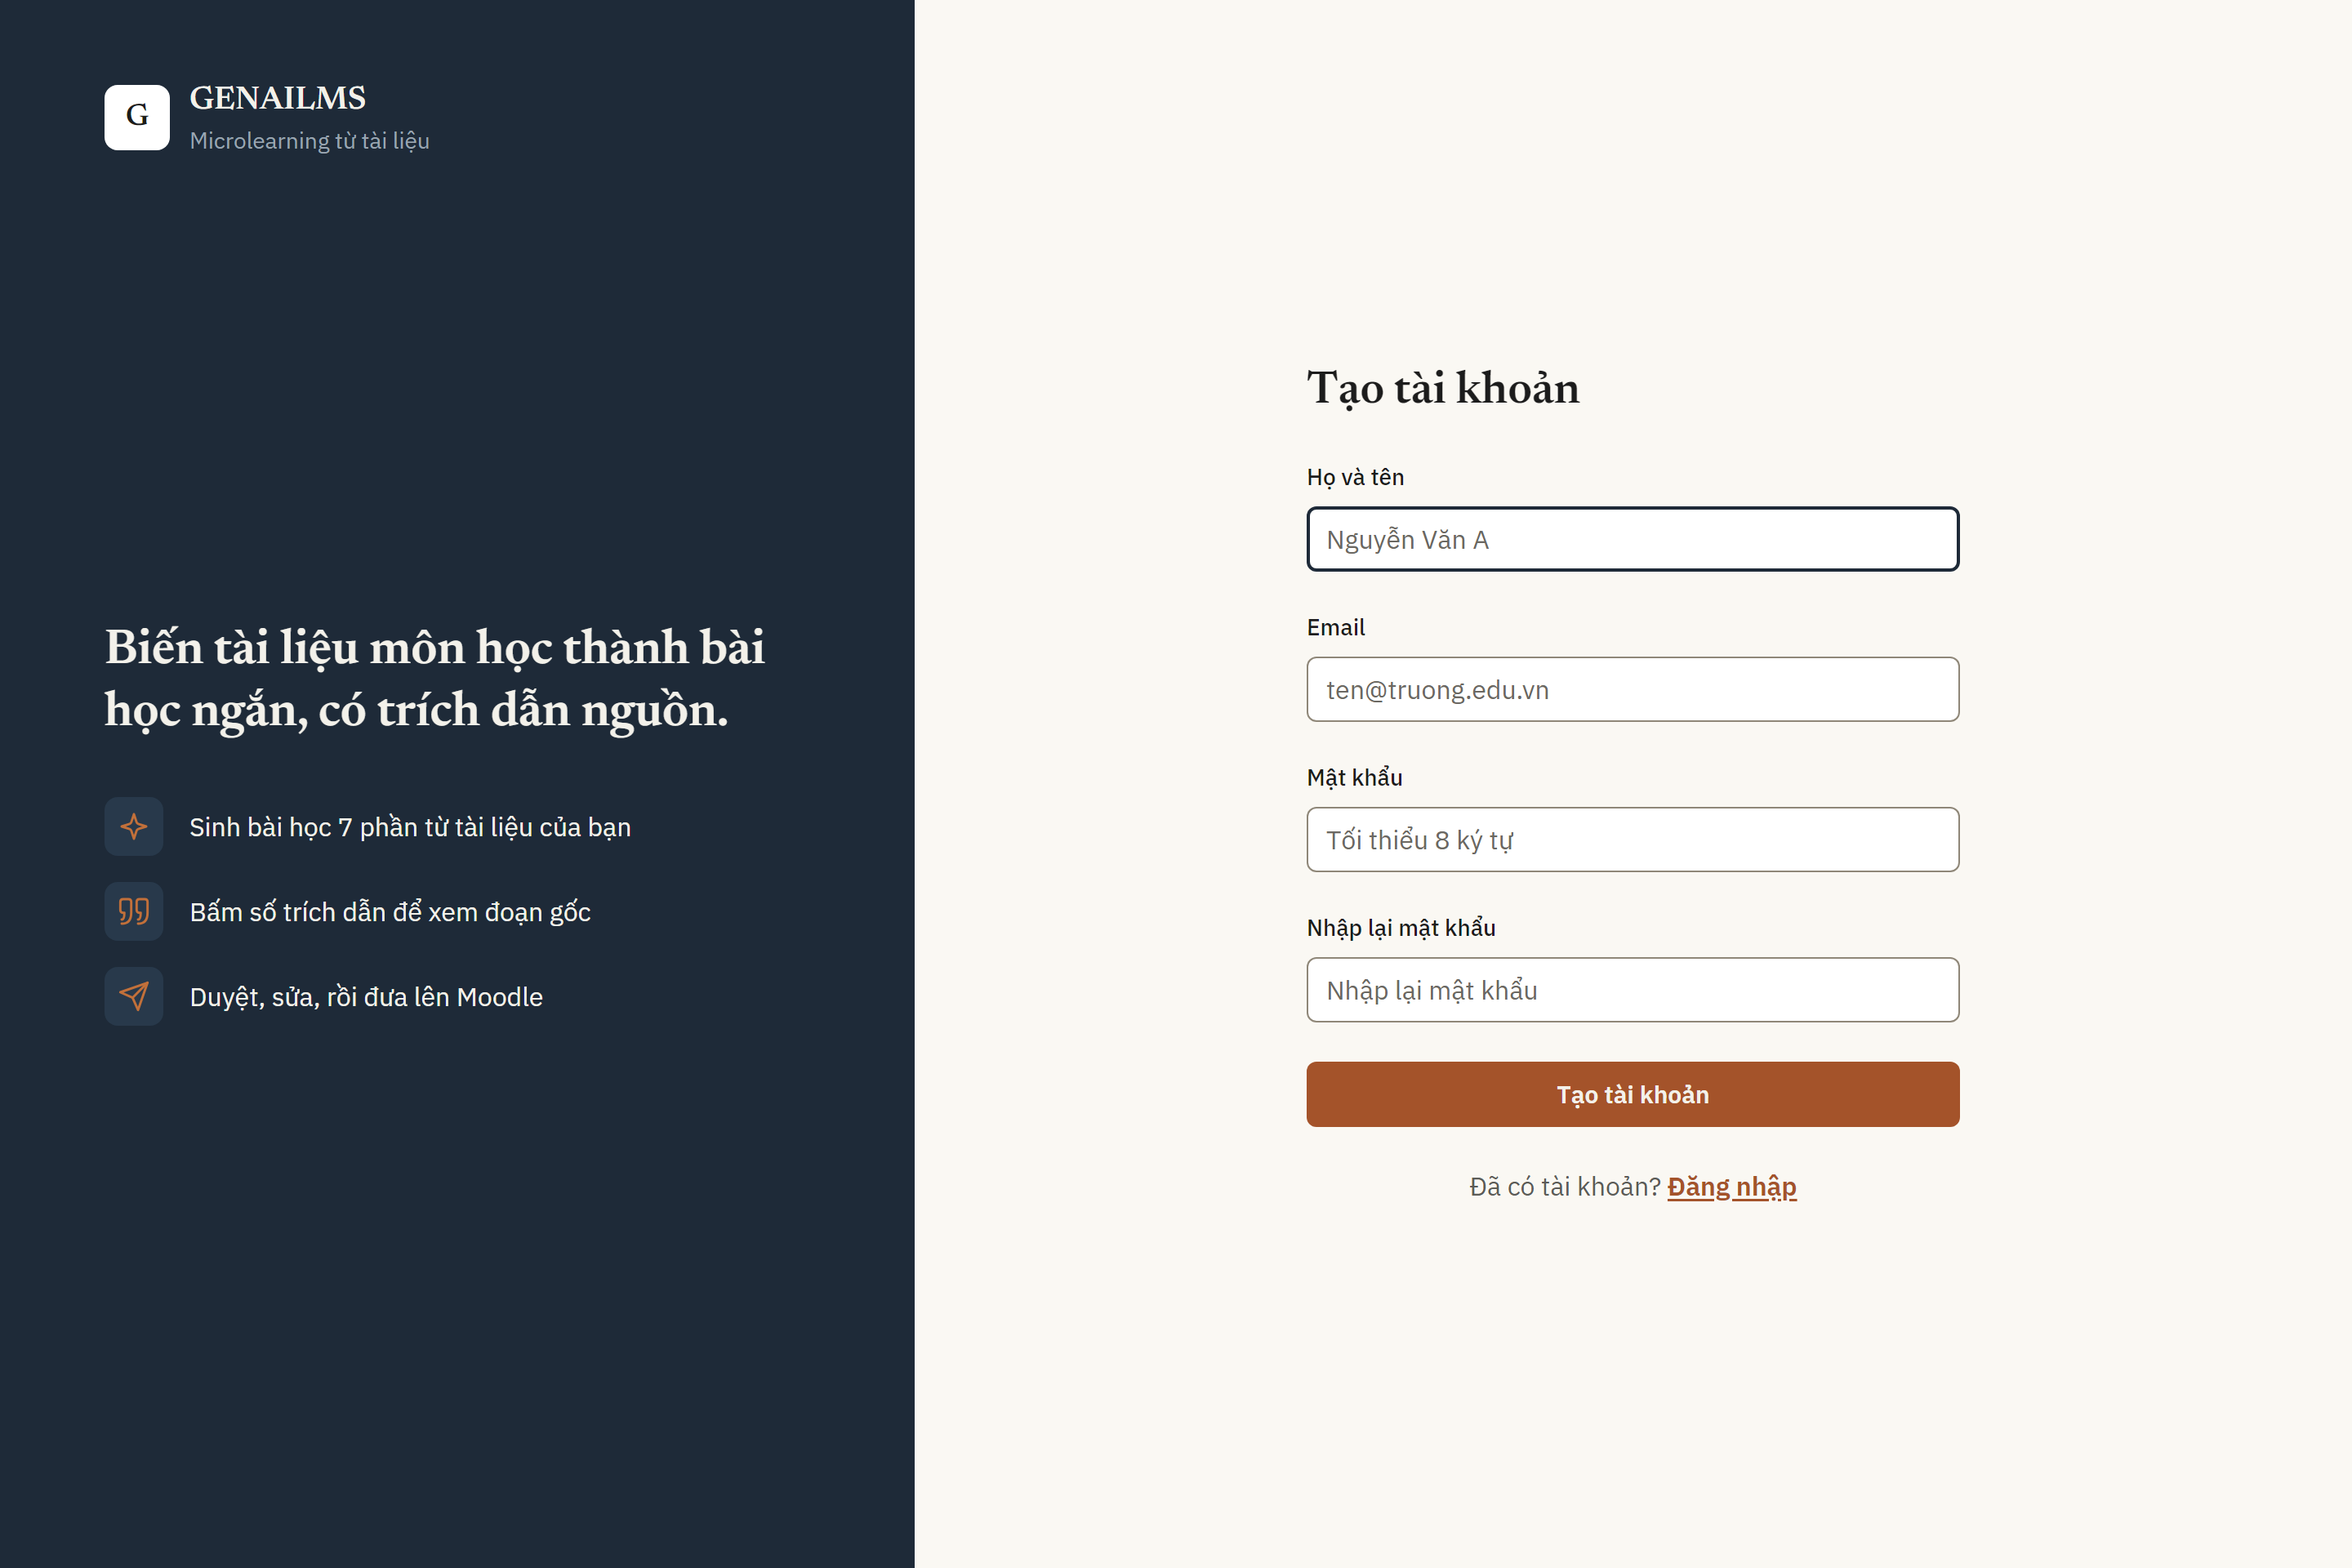
\includegraphics[width=\linewidth,height=.34\textheight,keepaspectratio,viewport={1560 420 2440 1010},clip]{graphics/ui/02-register.png}
\caption{Registration and labelled validation.}\label{fig:ui-screen-02}
\end{figure}

\needspace{.42\textheight}
Figure~\ref{fig:ui-screen-03} organizes the author's owned courses as selectable workspaces. ``Tạo môn học'' means ``Create course''; each card combines the course identity and a compact activity summary.
\begin{figure}[H]\centering
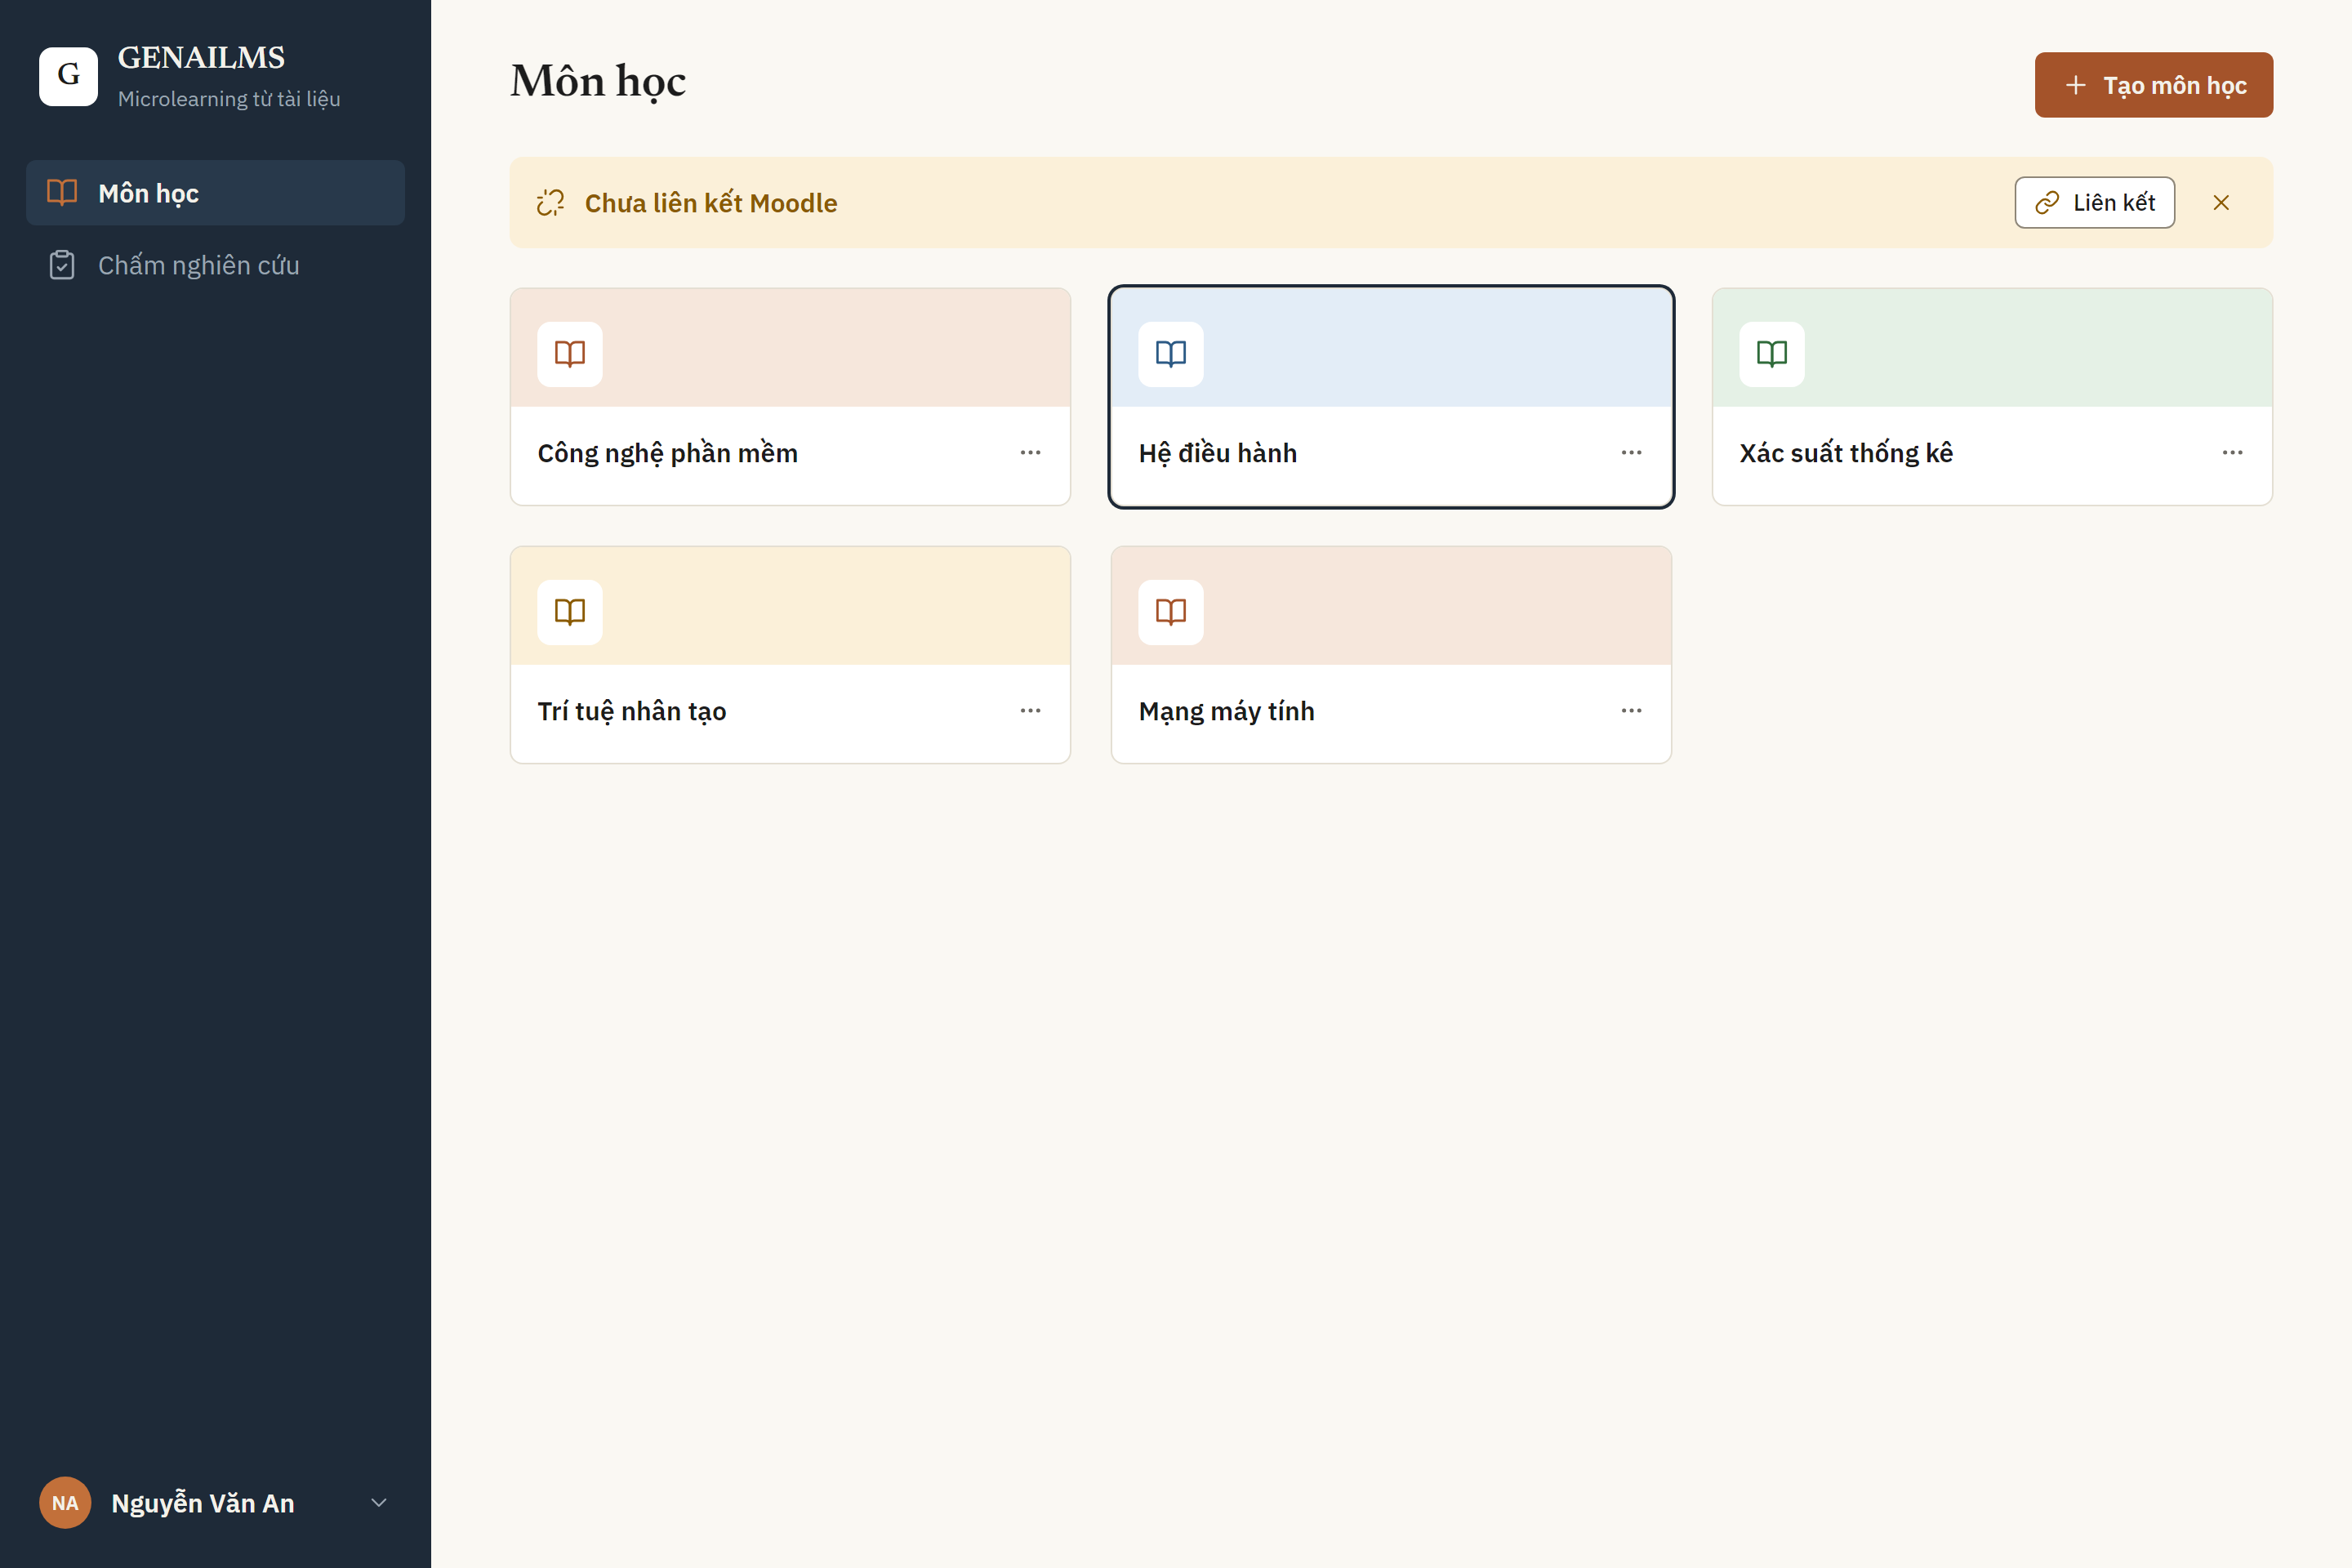
\includegraphics[width=\linewidth,height=.34\textheight,keepaspectratio,viewport={600 960 2070 1600},clip]{graphics/ui/03-course-list-dashboard.png}
\caption{Owned-course workspace selection.}\label{fig:ui-screen-03}
\end{figure}

\needspace{.42\textheight}
The workspace in Figure~\ref{fig:ui-screen-04} combines document status, generation actions and course context. ``Sẵn sàng'' means ``Ready'', while ``Đang xử lý'' means ``Processing''; course Q\&A is entered from this owned-workspace context.
\begin{figure}[H]\centering
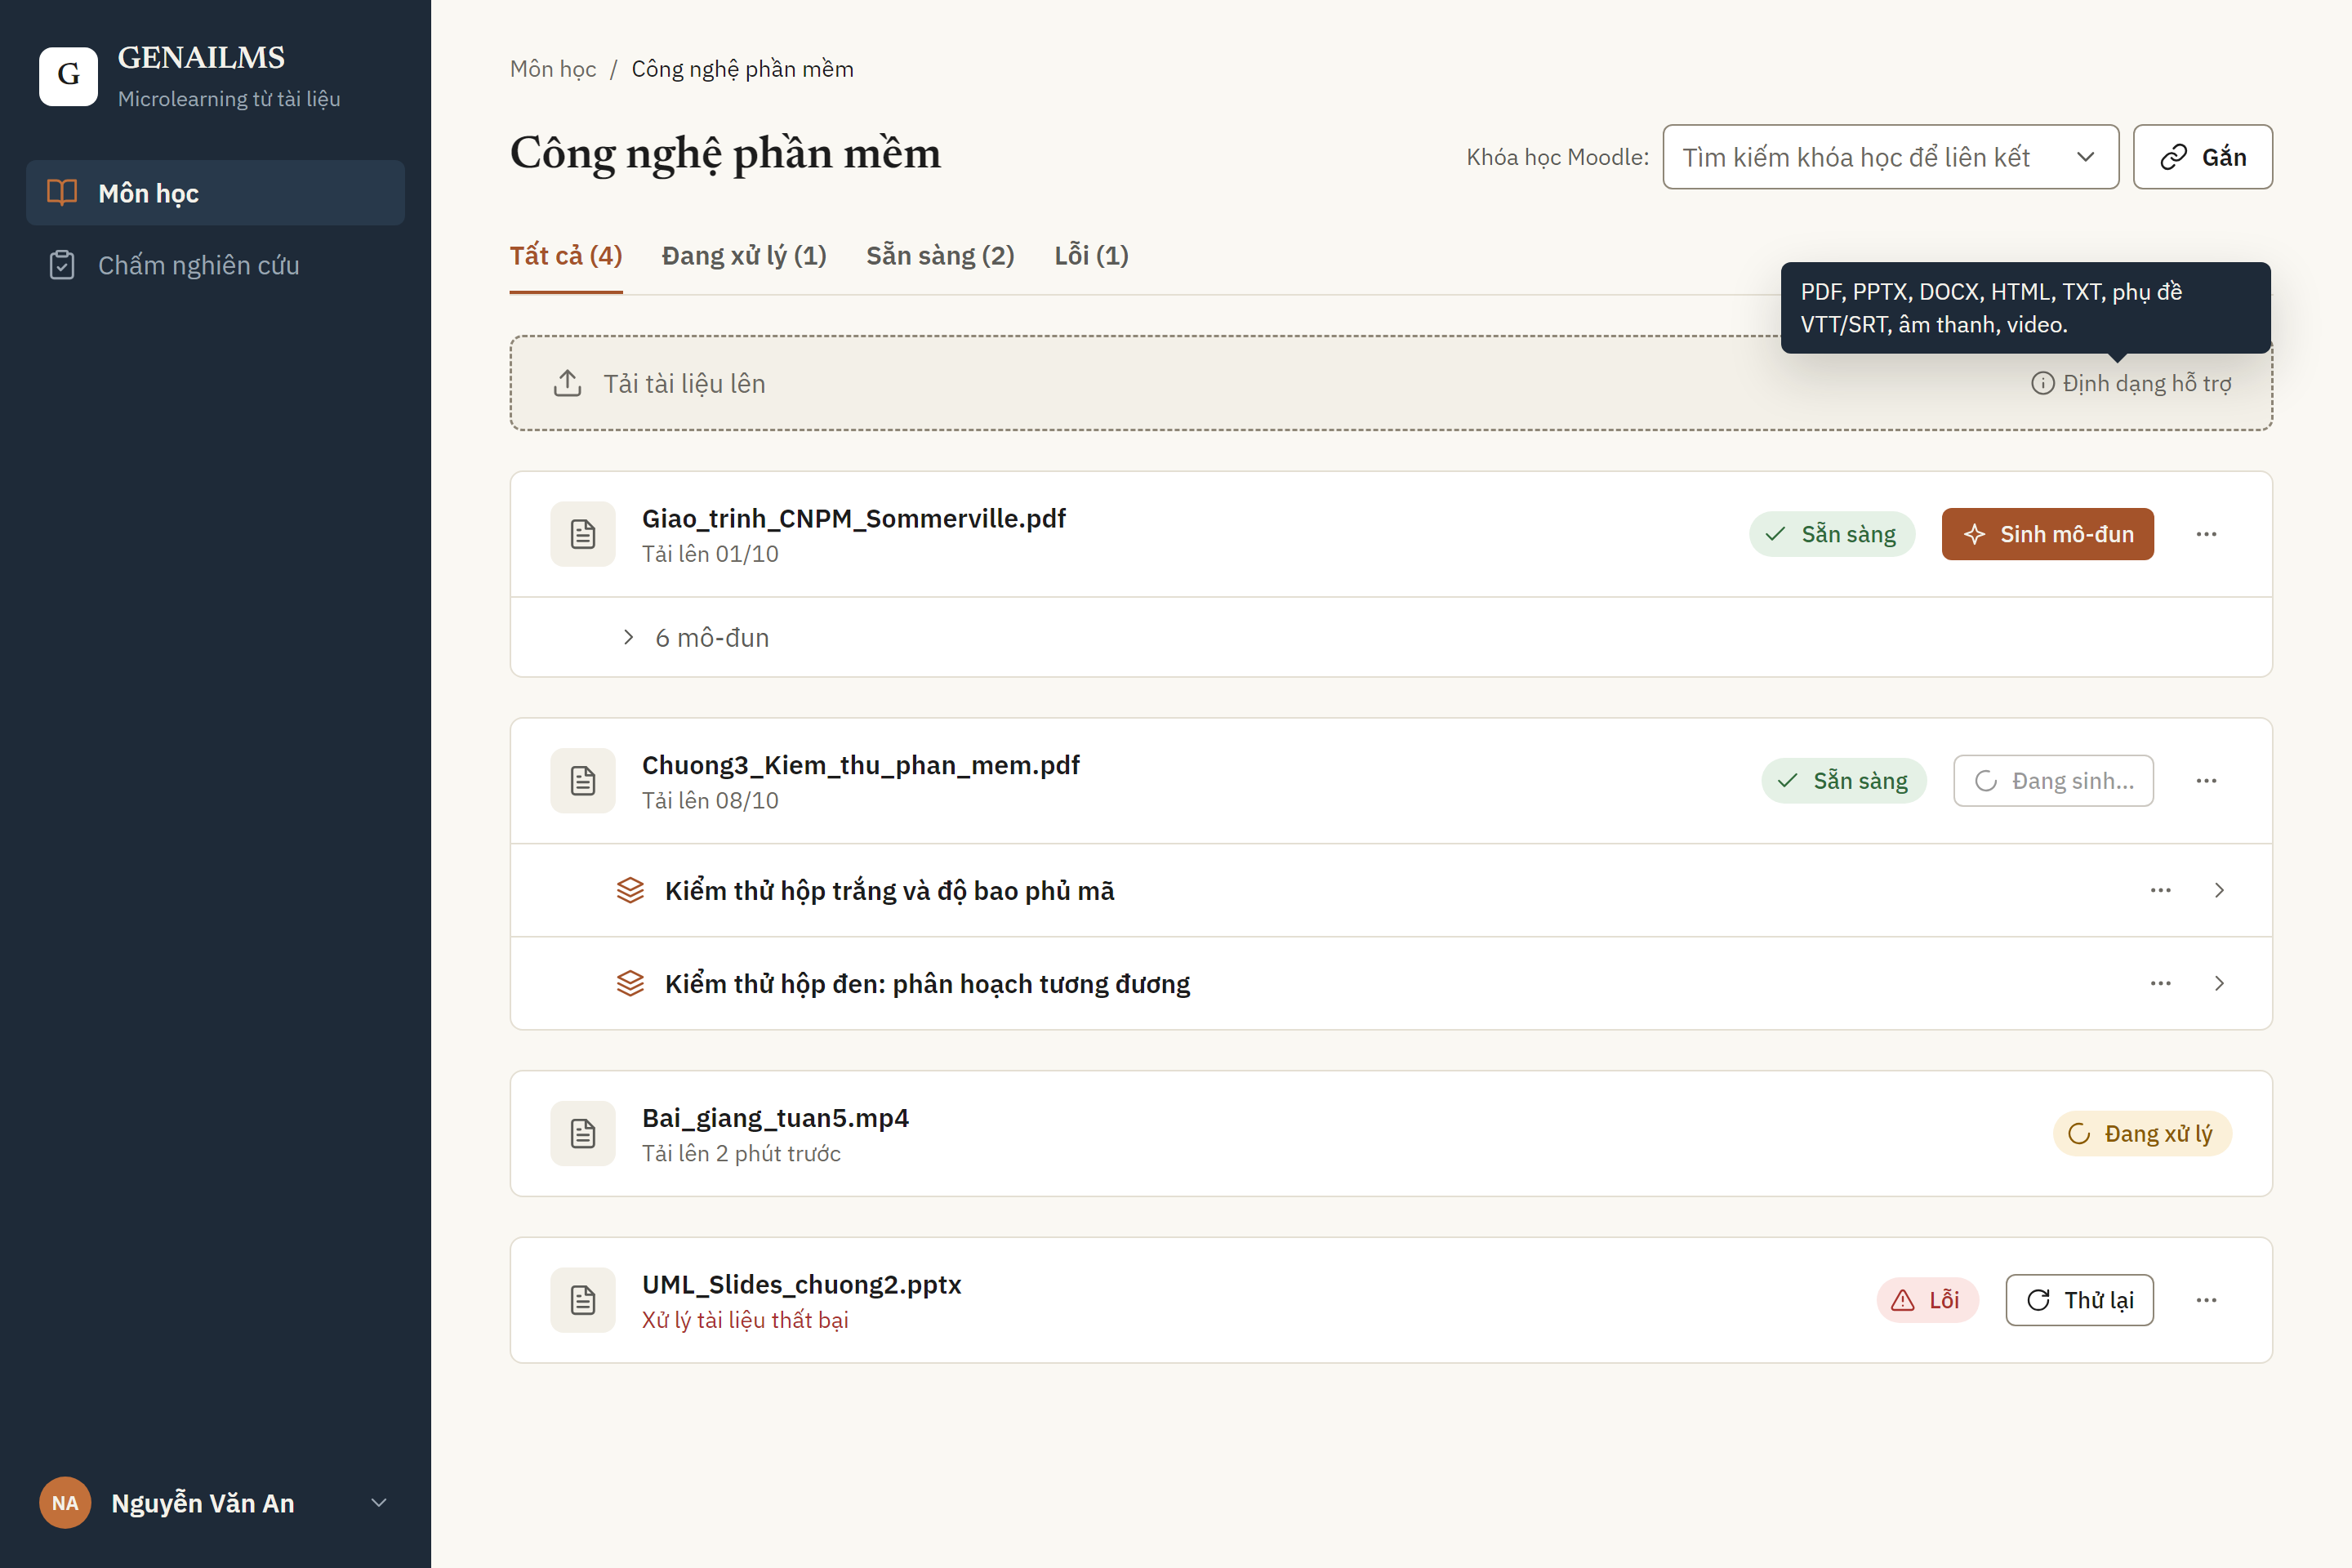
\includegraphics[width=\linewidth,height=.34\textheight,keepaspectratio,viewport={590 600 2820 1800},clip]{graphics/ui/04-course-detail.png}
\caption{Course documents and processing feedback.}\label{fig:ui-screen-04}
\end{figure}

\needspace{.42\textheight}
Figure~\ref{fig:ui-screen-05} asks the author to confirm a model, output language and additional guidance before generation. ``Mặc định'' means ``Default'' and ``Sinh mô-đun'' means ``Generate module''; the saved preference preselects the model without preventing a one-request override.
\begin{figure}[H]\centering
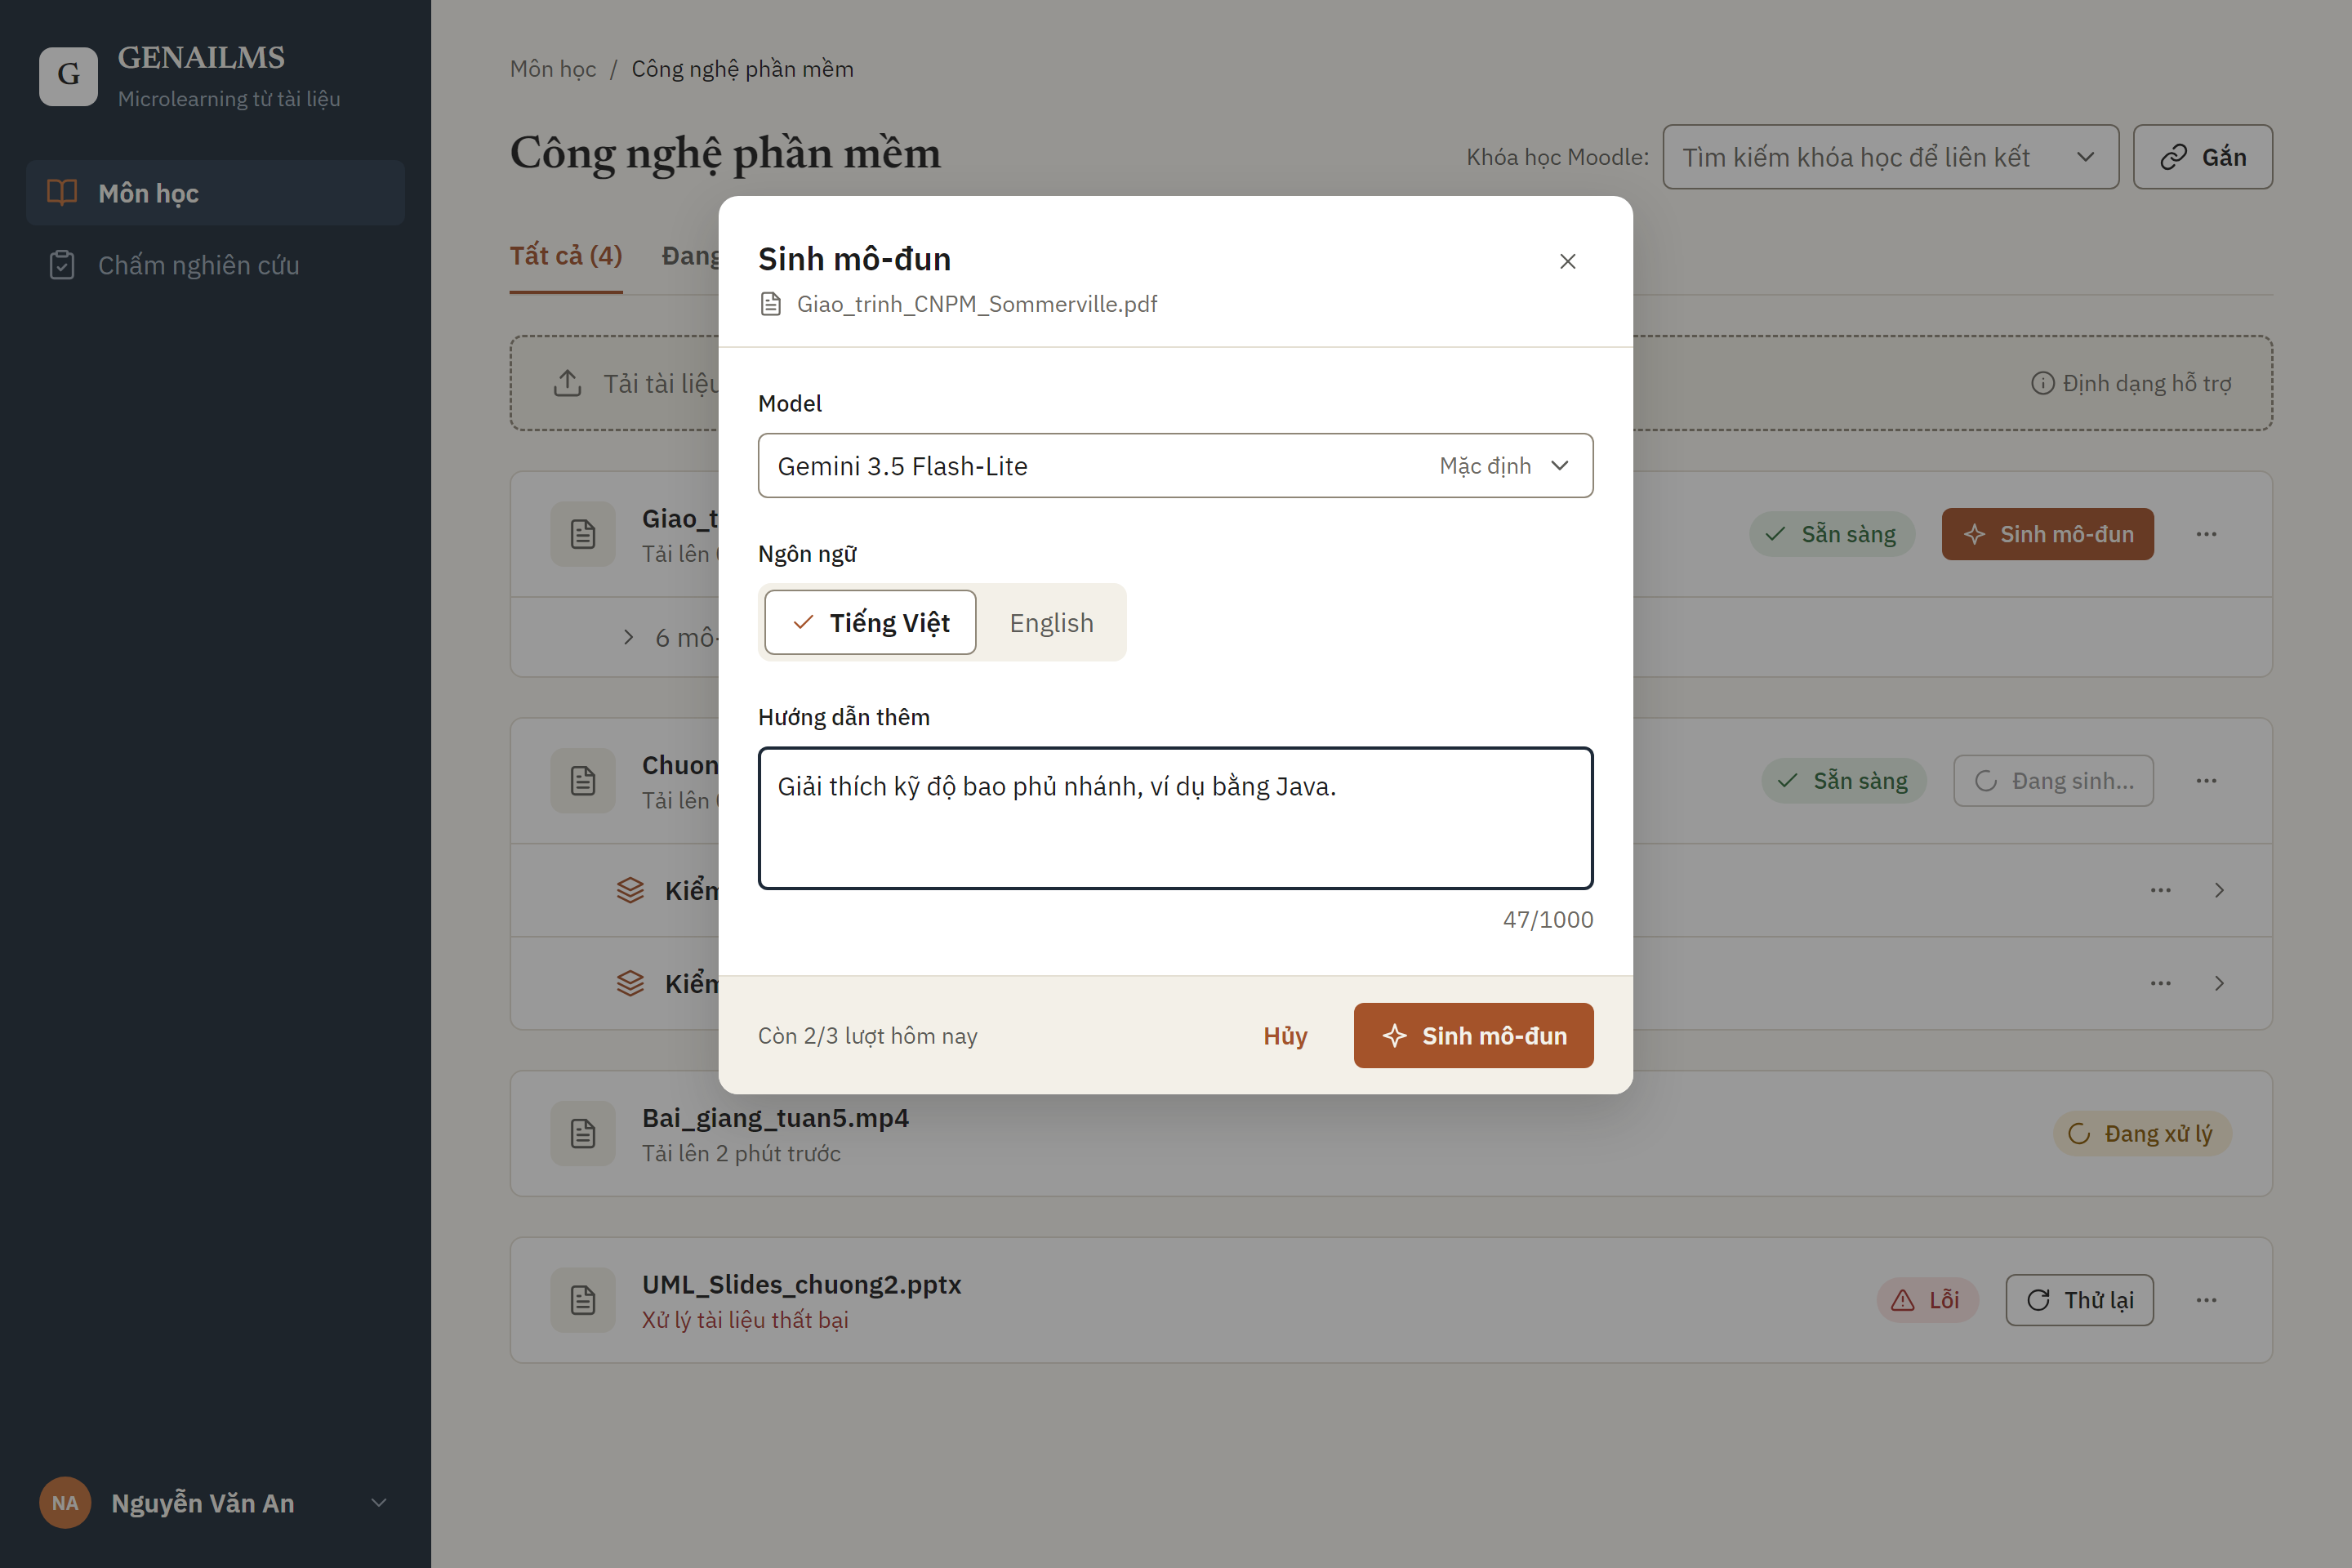
\includegraphics[width=\linewidth,height=.42\textheight,keepaspectratio,viewport={900 585 1980 1510},clip]{graphics/ui/05-generate-module-dialog.png}
\caption{Generation choices before submitting a job.}\label{fig:ui-screen-05}
\end{figure}

\needspace{.42\textheight}
Figure~\ref{fig:ui-screen-06} enlarges the highlighted claim and its source panel as two views of the same screen. ``Nguồn'' means ``Sources'' and ``Khớp'' means ``Matched''; an unresolved source remains visible for review rather than receiving a fabricated match.
\begin{figure}[H]\centering
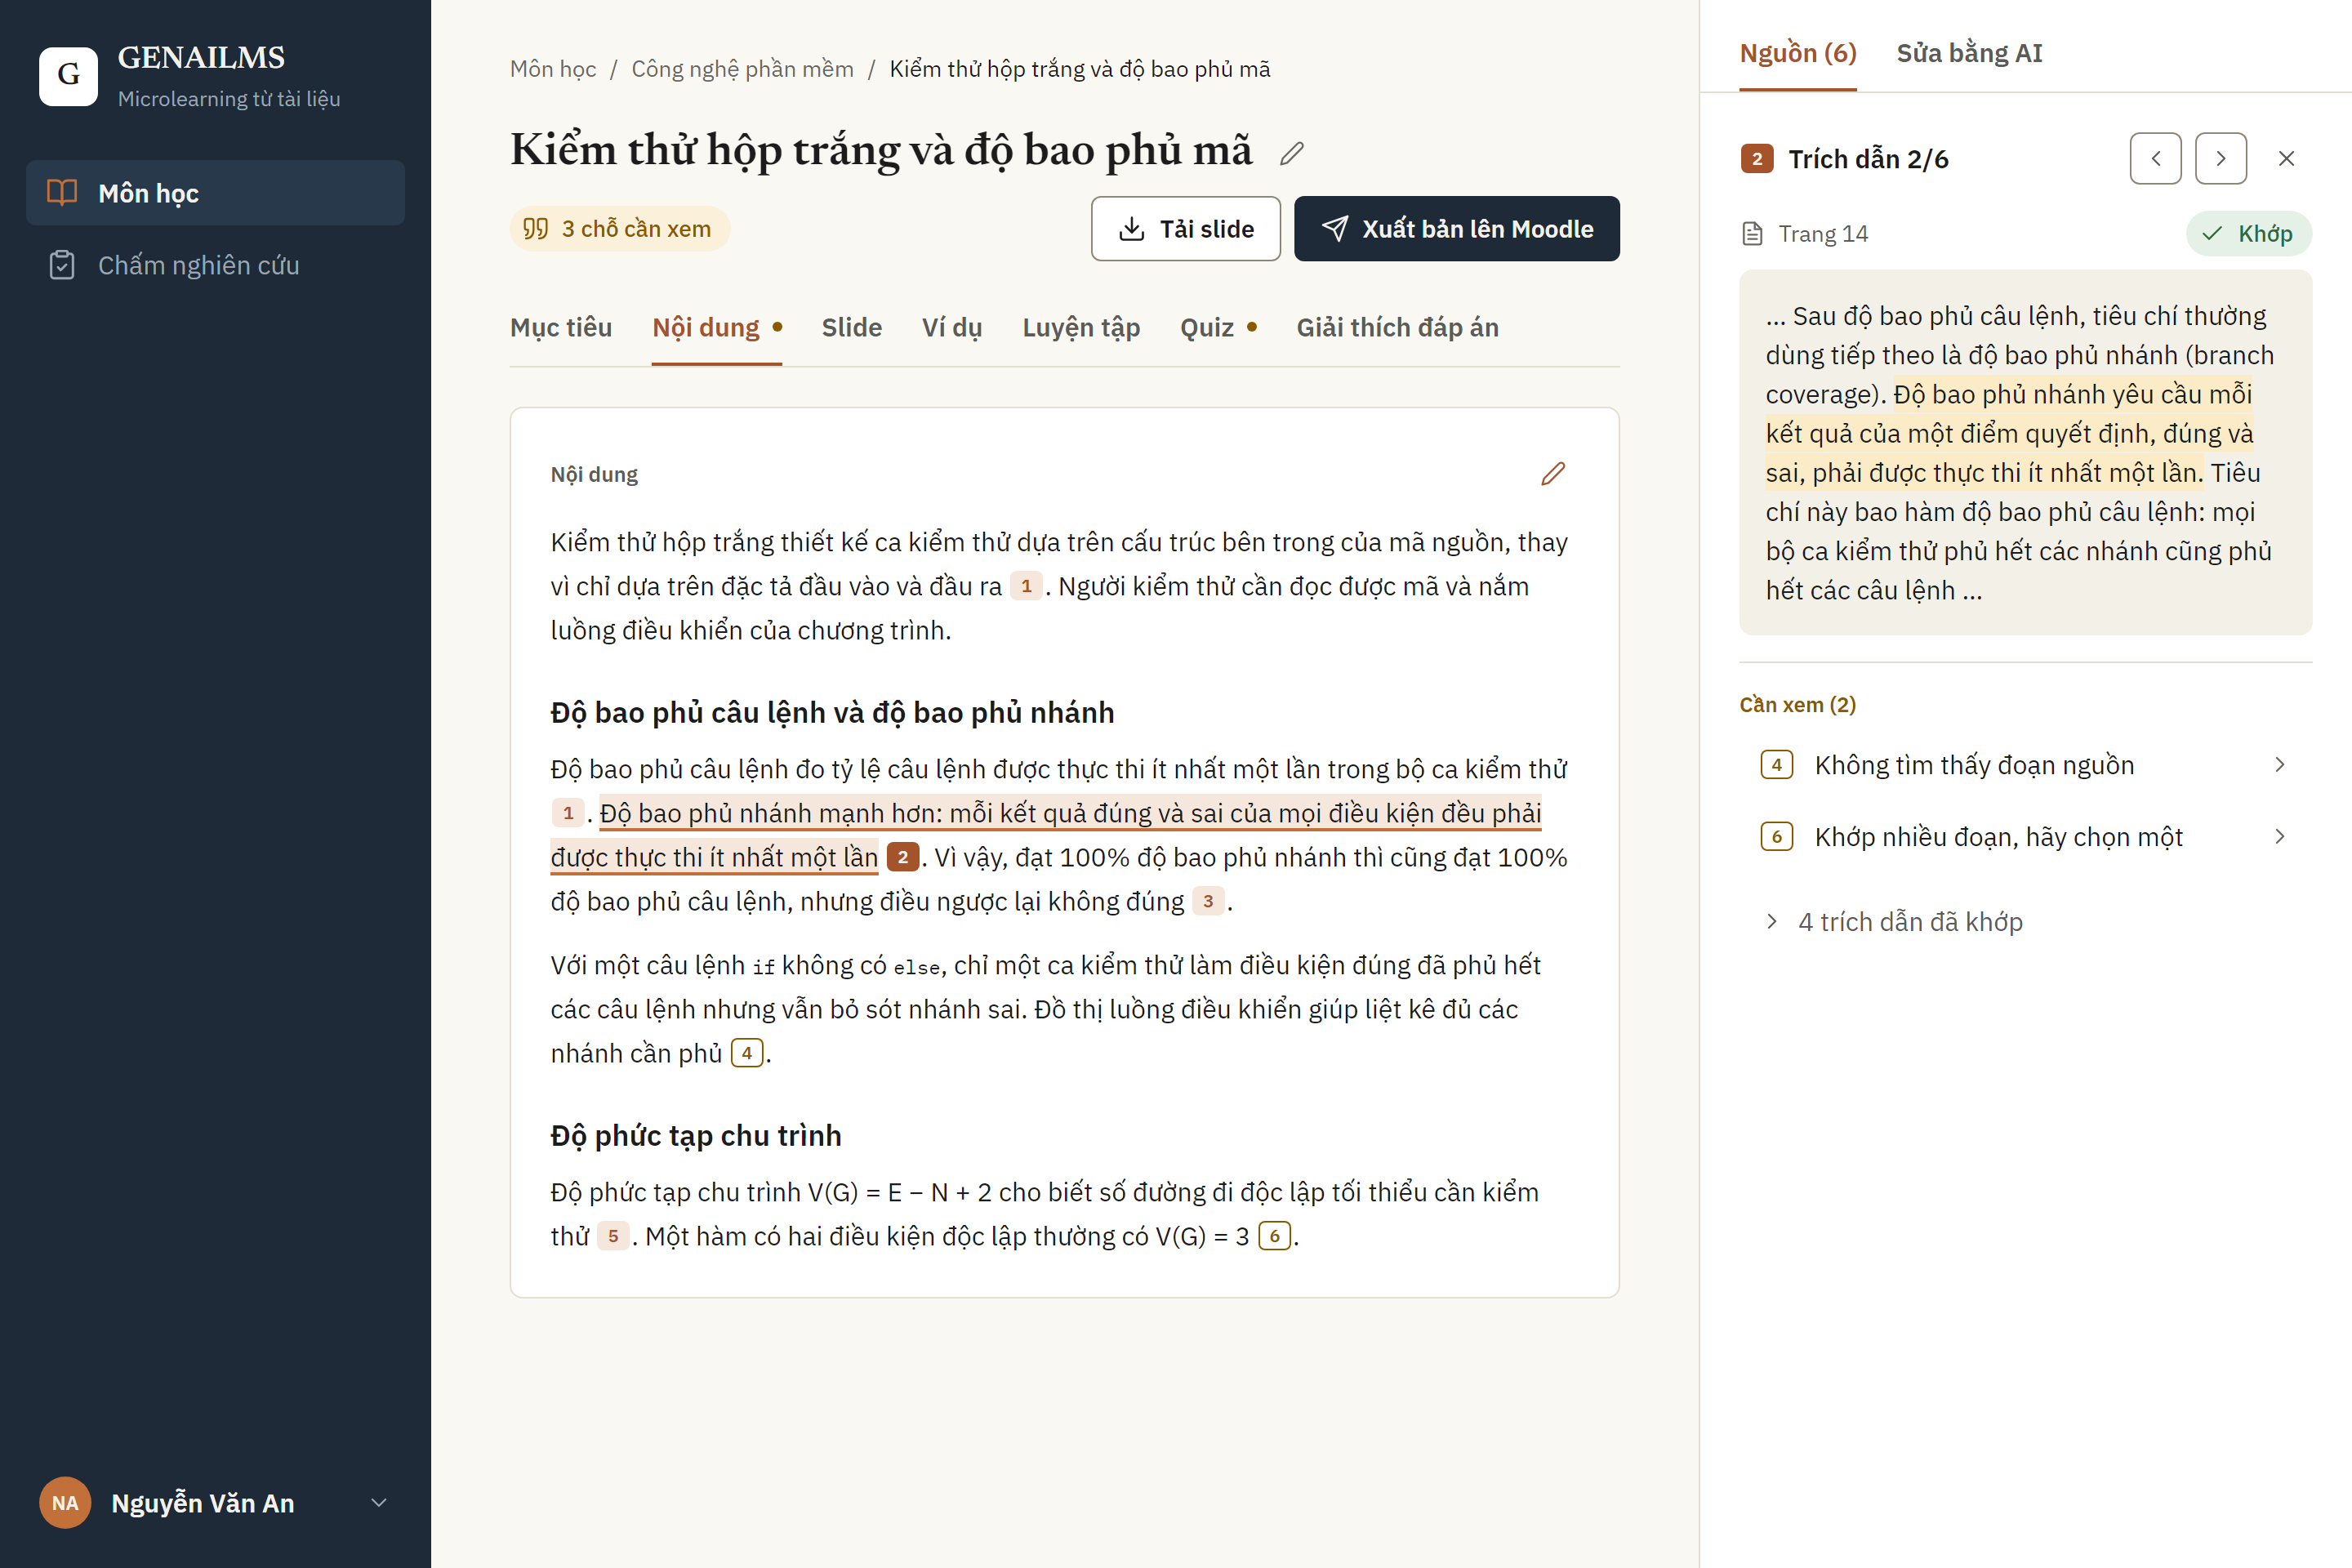
\includegraphics[width=\linewidth,height=.27\textheight,keepaspectratio,viewport={650 570 2000 1150},clip]{graphics/ui/06-module-editor-citations.png}\par\smallskip
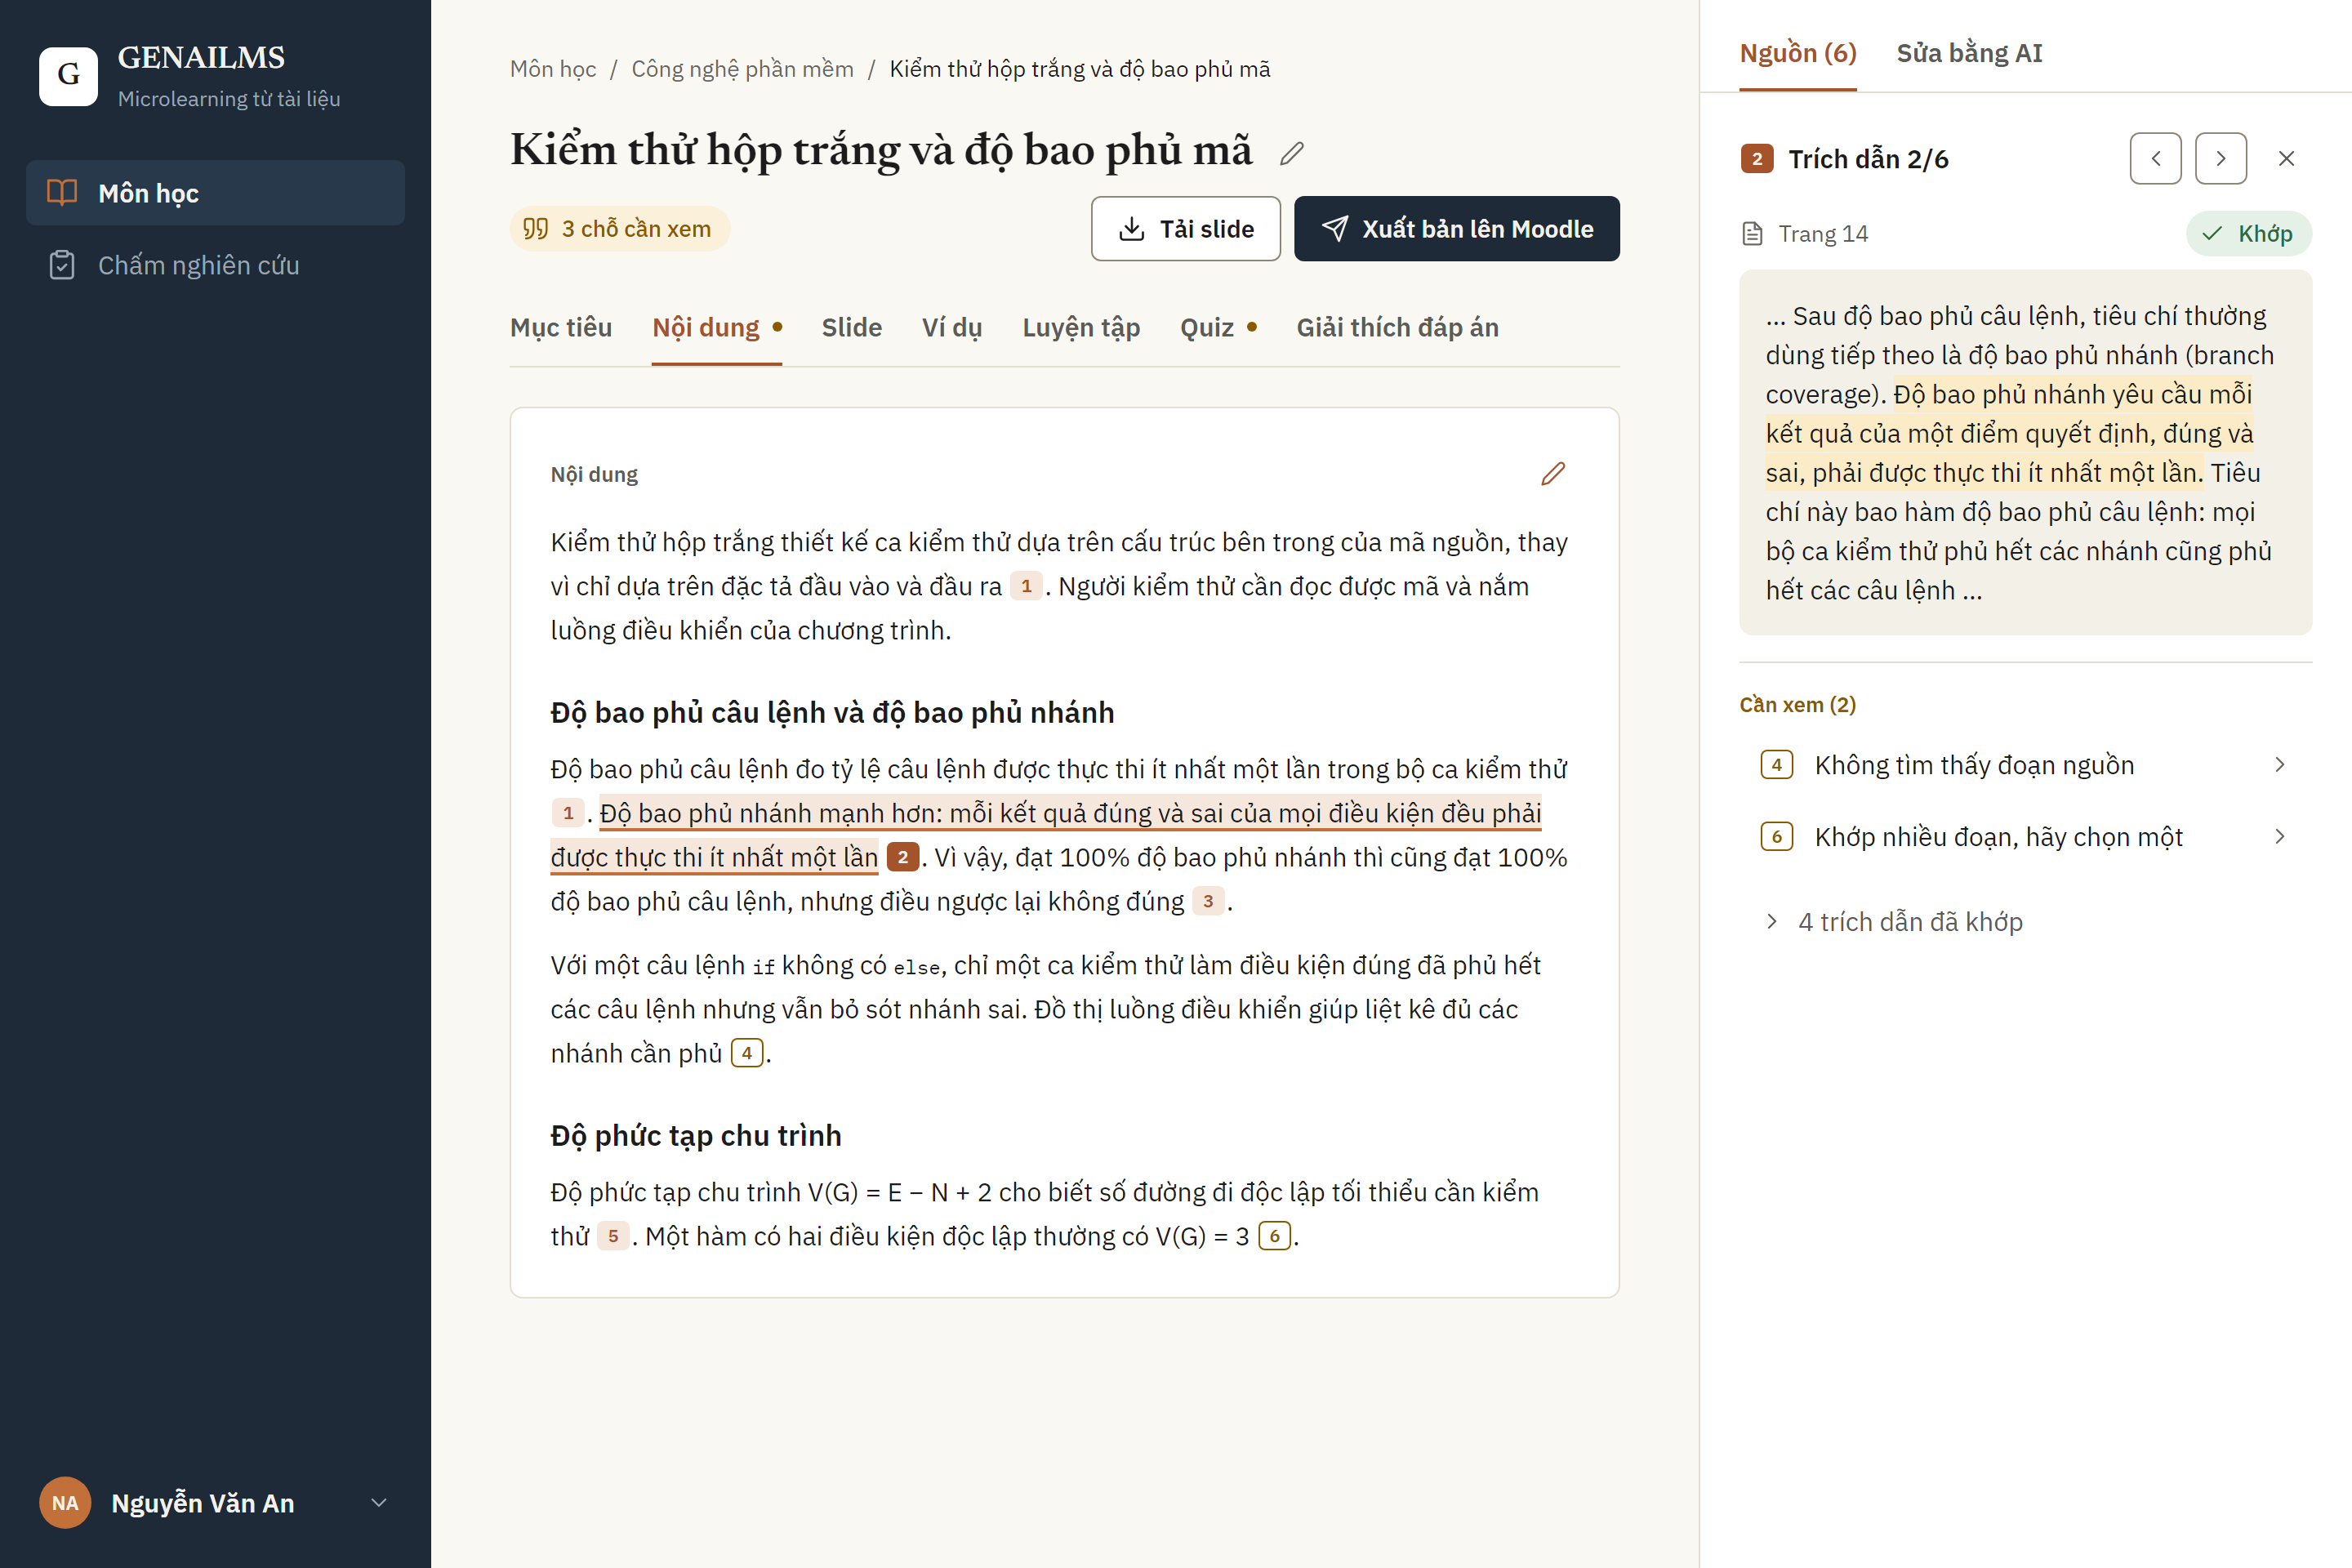
\includegraphics[width=\linewidth,height=.27\textheight,keepaspectratio,viewport={2080 1120 2850 1800},clip]{graphics/ui/06-module-editor-citations.png}
\caption{Claim marker and corresponding physical source passage.}\label{fig:ui-screen-06}
\end{figure}

\needspace{.42\textheight}
The contextual panel in Figure~\ref{fig:ui-screen-07} accepts a component-edit request while retaining the lesson context. ``Sửa bằng AI'' means ``Edit with AI''; accepting an edit follows the same validation and original-preservation contract as a manual change.
\begin{figure}[H]\centering
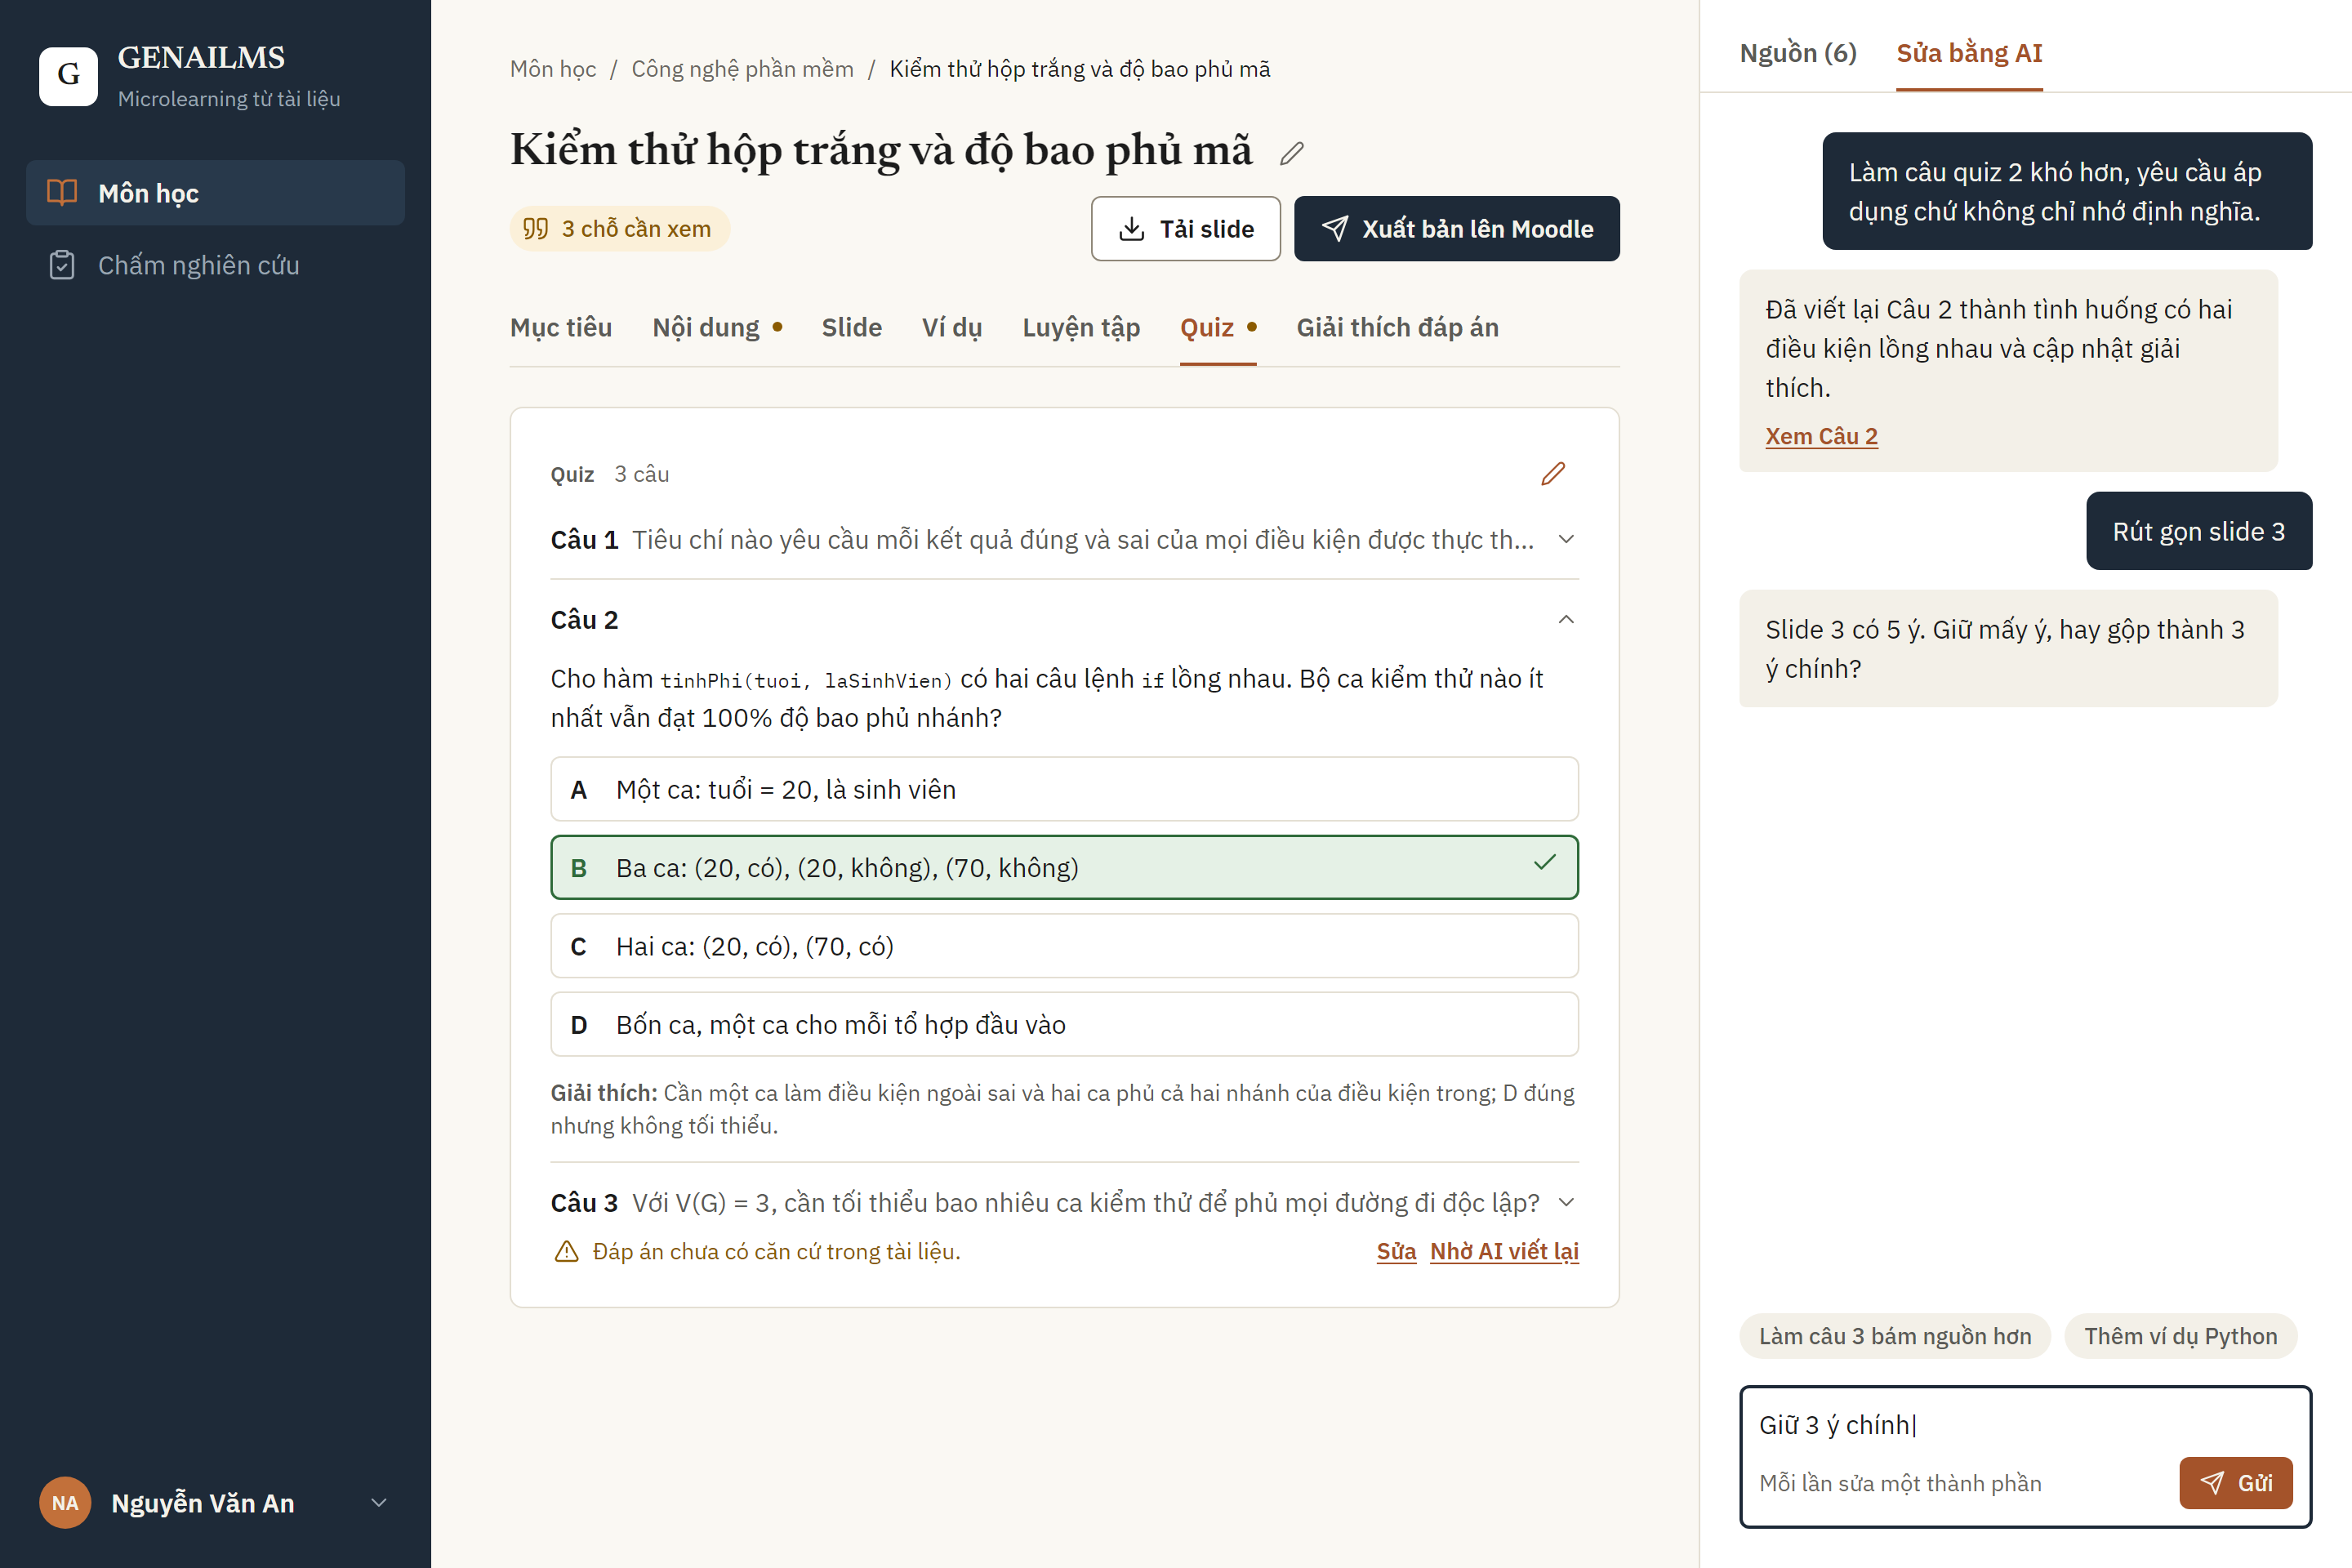
\includegraphics[width=\linewidth,height=.34\textheight,keepaspectratio,viewport={2100 1320 2850 1780},clip]{graphics/ui/07-module-editor-chat-edit.png}
\caption{Contextual editing request and response.}\label{fig:ui-screen-07}
\end{figure}

\needspace{.42\textheight}
Figure~\ref{fig:ui-screen-08} makes the target course/section and activity selection visible before publication. ``Xuất bản lên Moodle'' means ``Publish to Moodle''; the explicit confirmation reduces accidental publication to a remembered destination.
\begin{figure}[H]\centering
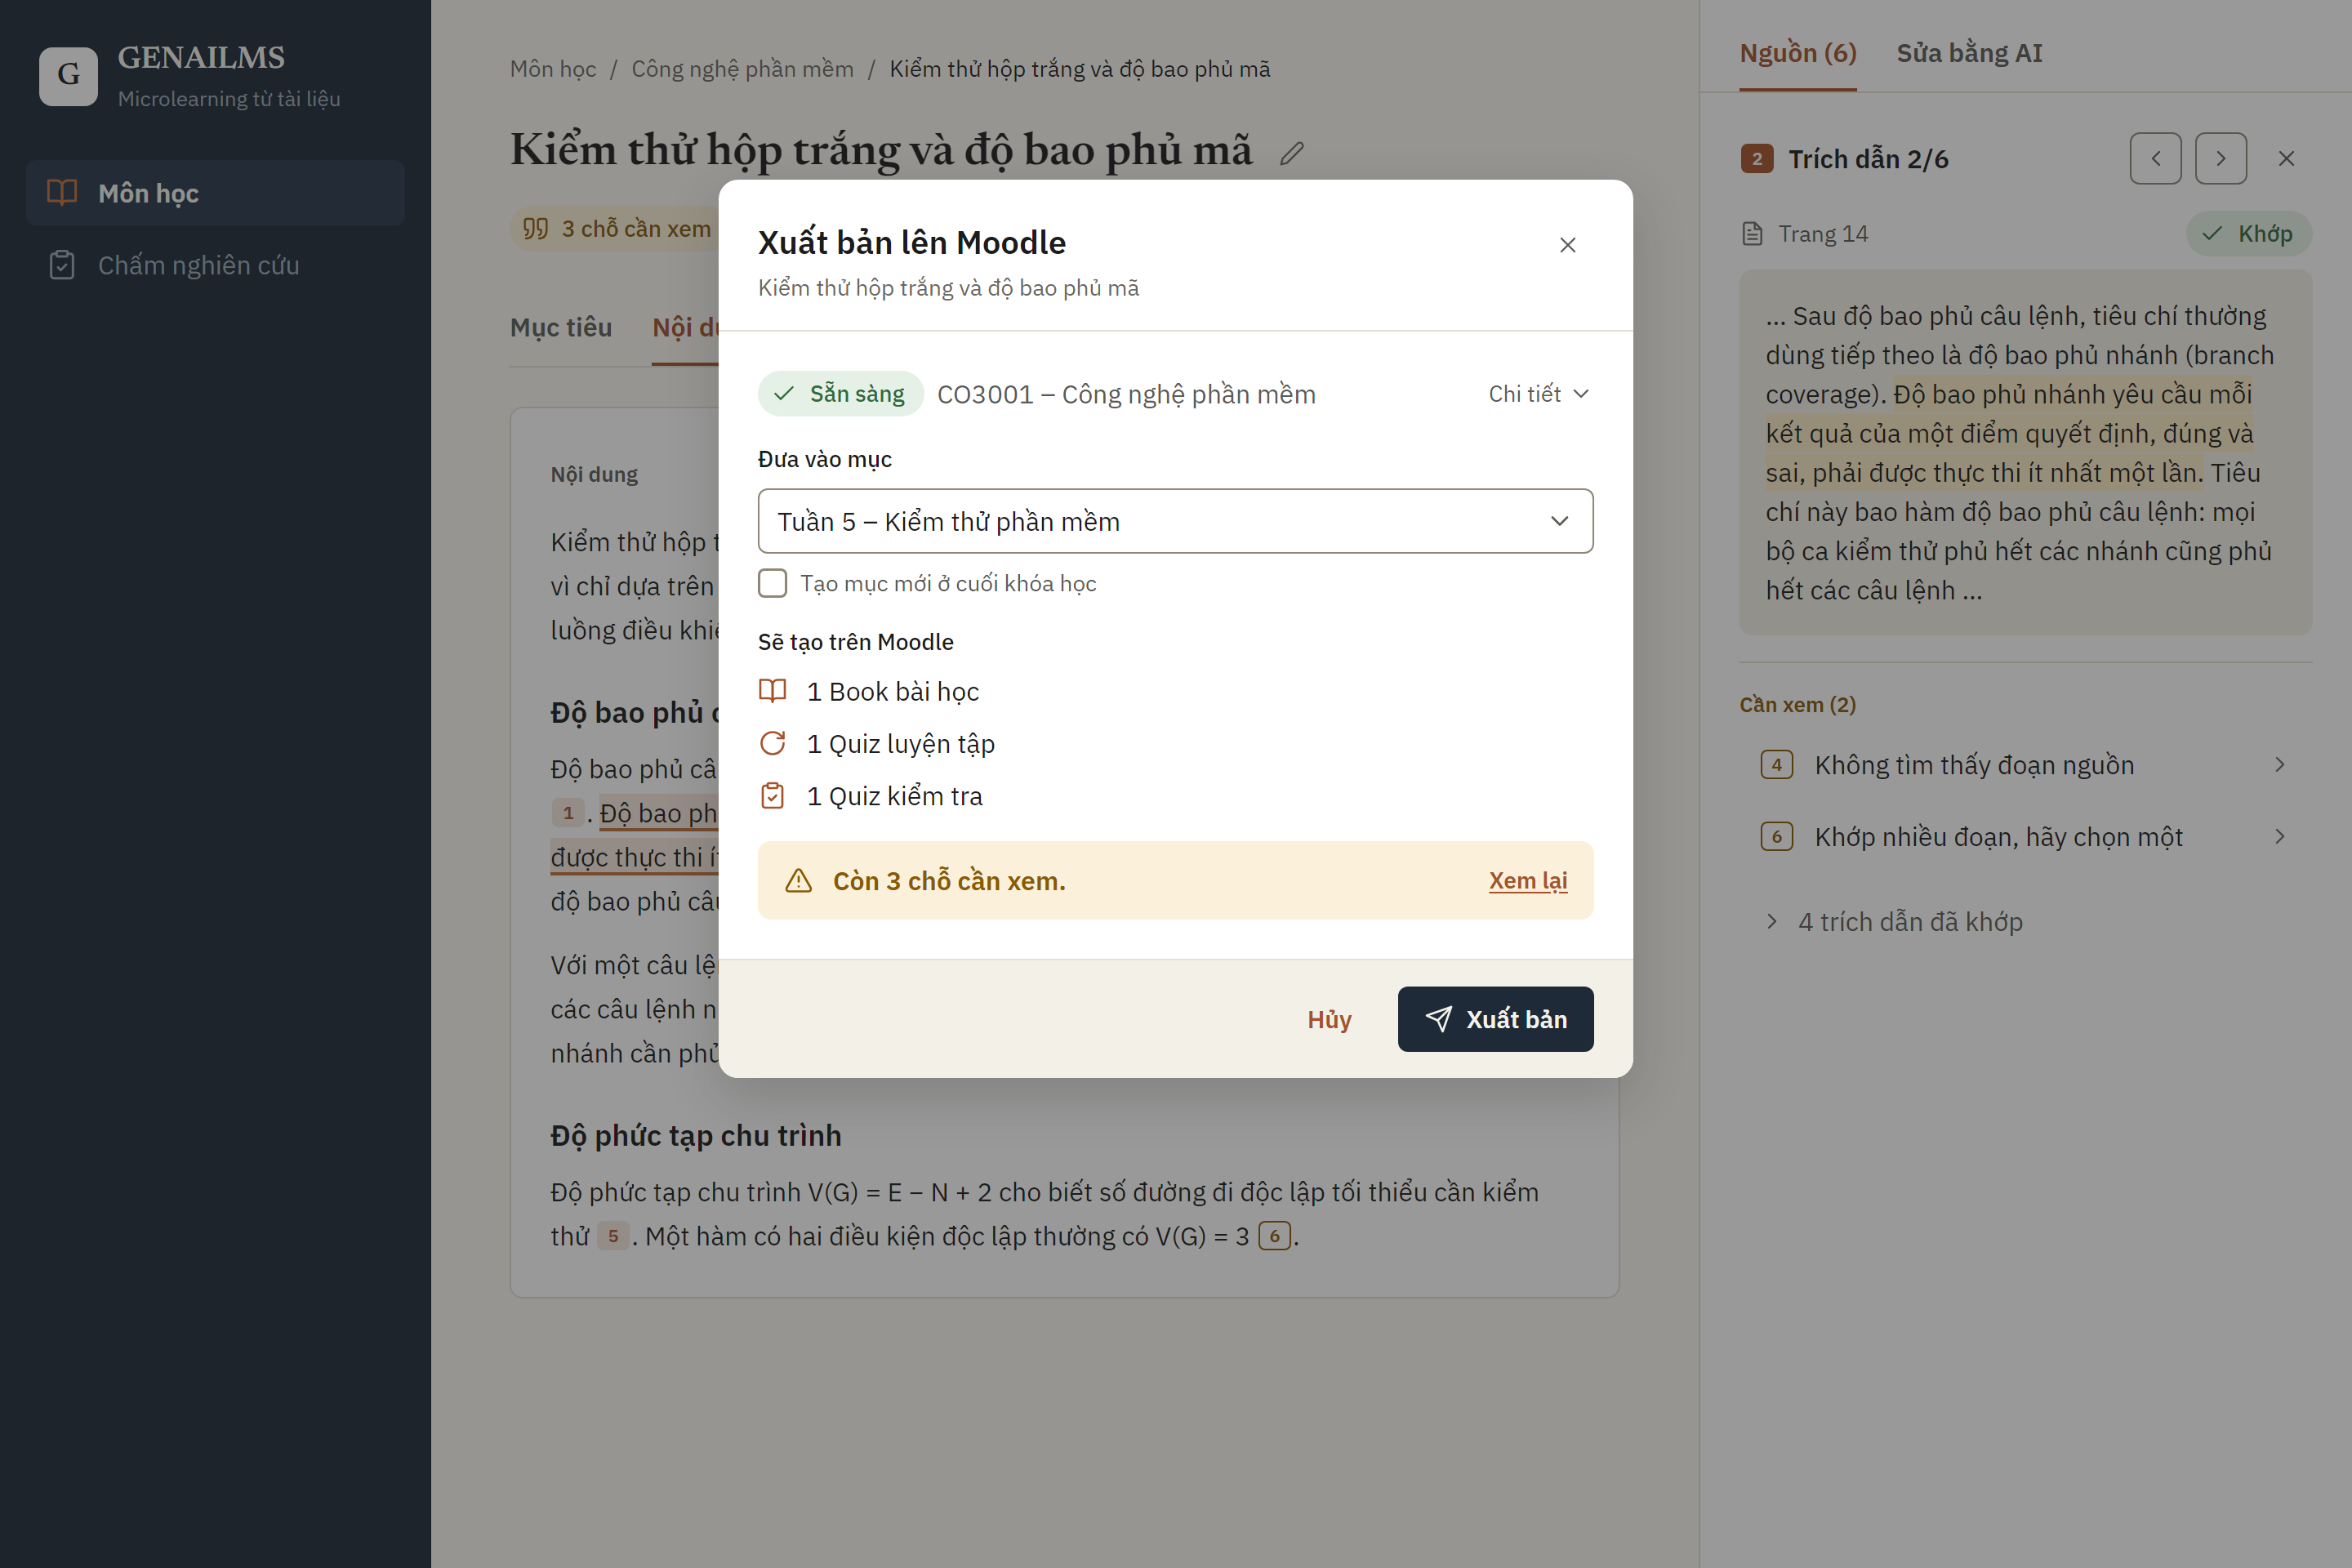
\includegraphics[width=\linewidth,height=.42\textheight,keepaspectratio,viewport={900 600 1980 1510},clip]{graphics/ui/08-publish-to-moodle.png}
\caption{Publication destination and activity review.}\label{fig:ui-screen-08}
\end{figure}

\needspace{.42\textheight}
Figure~\ref{fig:ui-screen-09} highlights pending identity confirmation and its next action. Account linking and course permission remain separate states; subsequent publication verifies the target-course capabilities without exposing account existence through the generic link-request response.
\begin{figure}[H]\centering
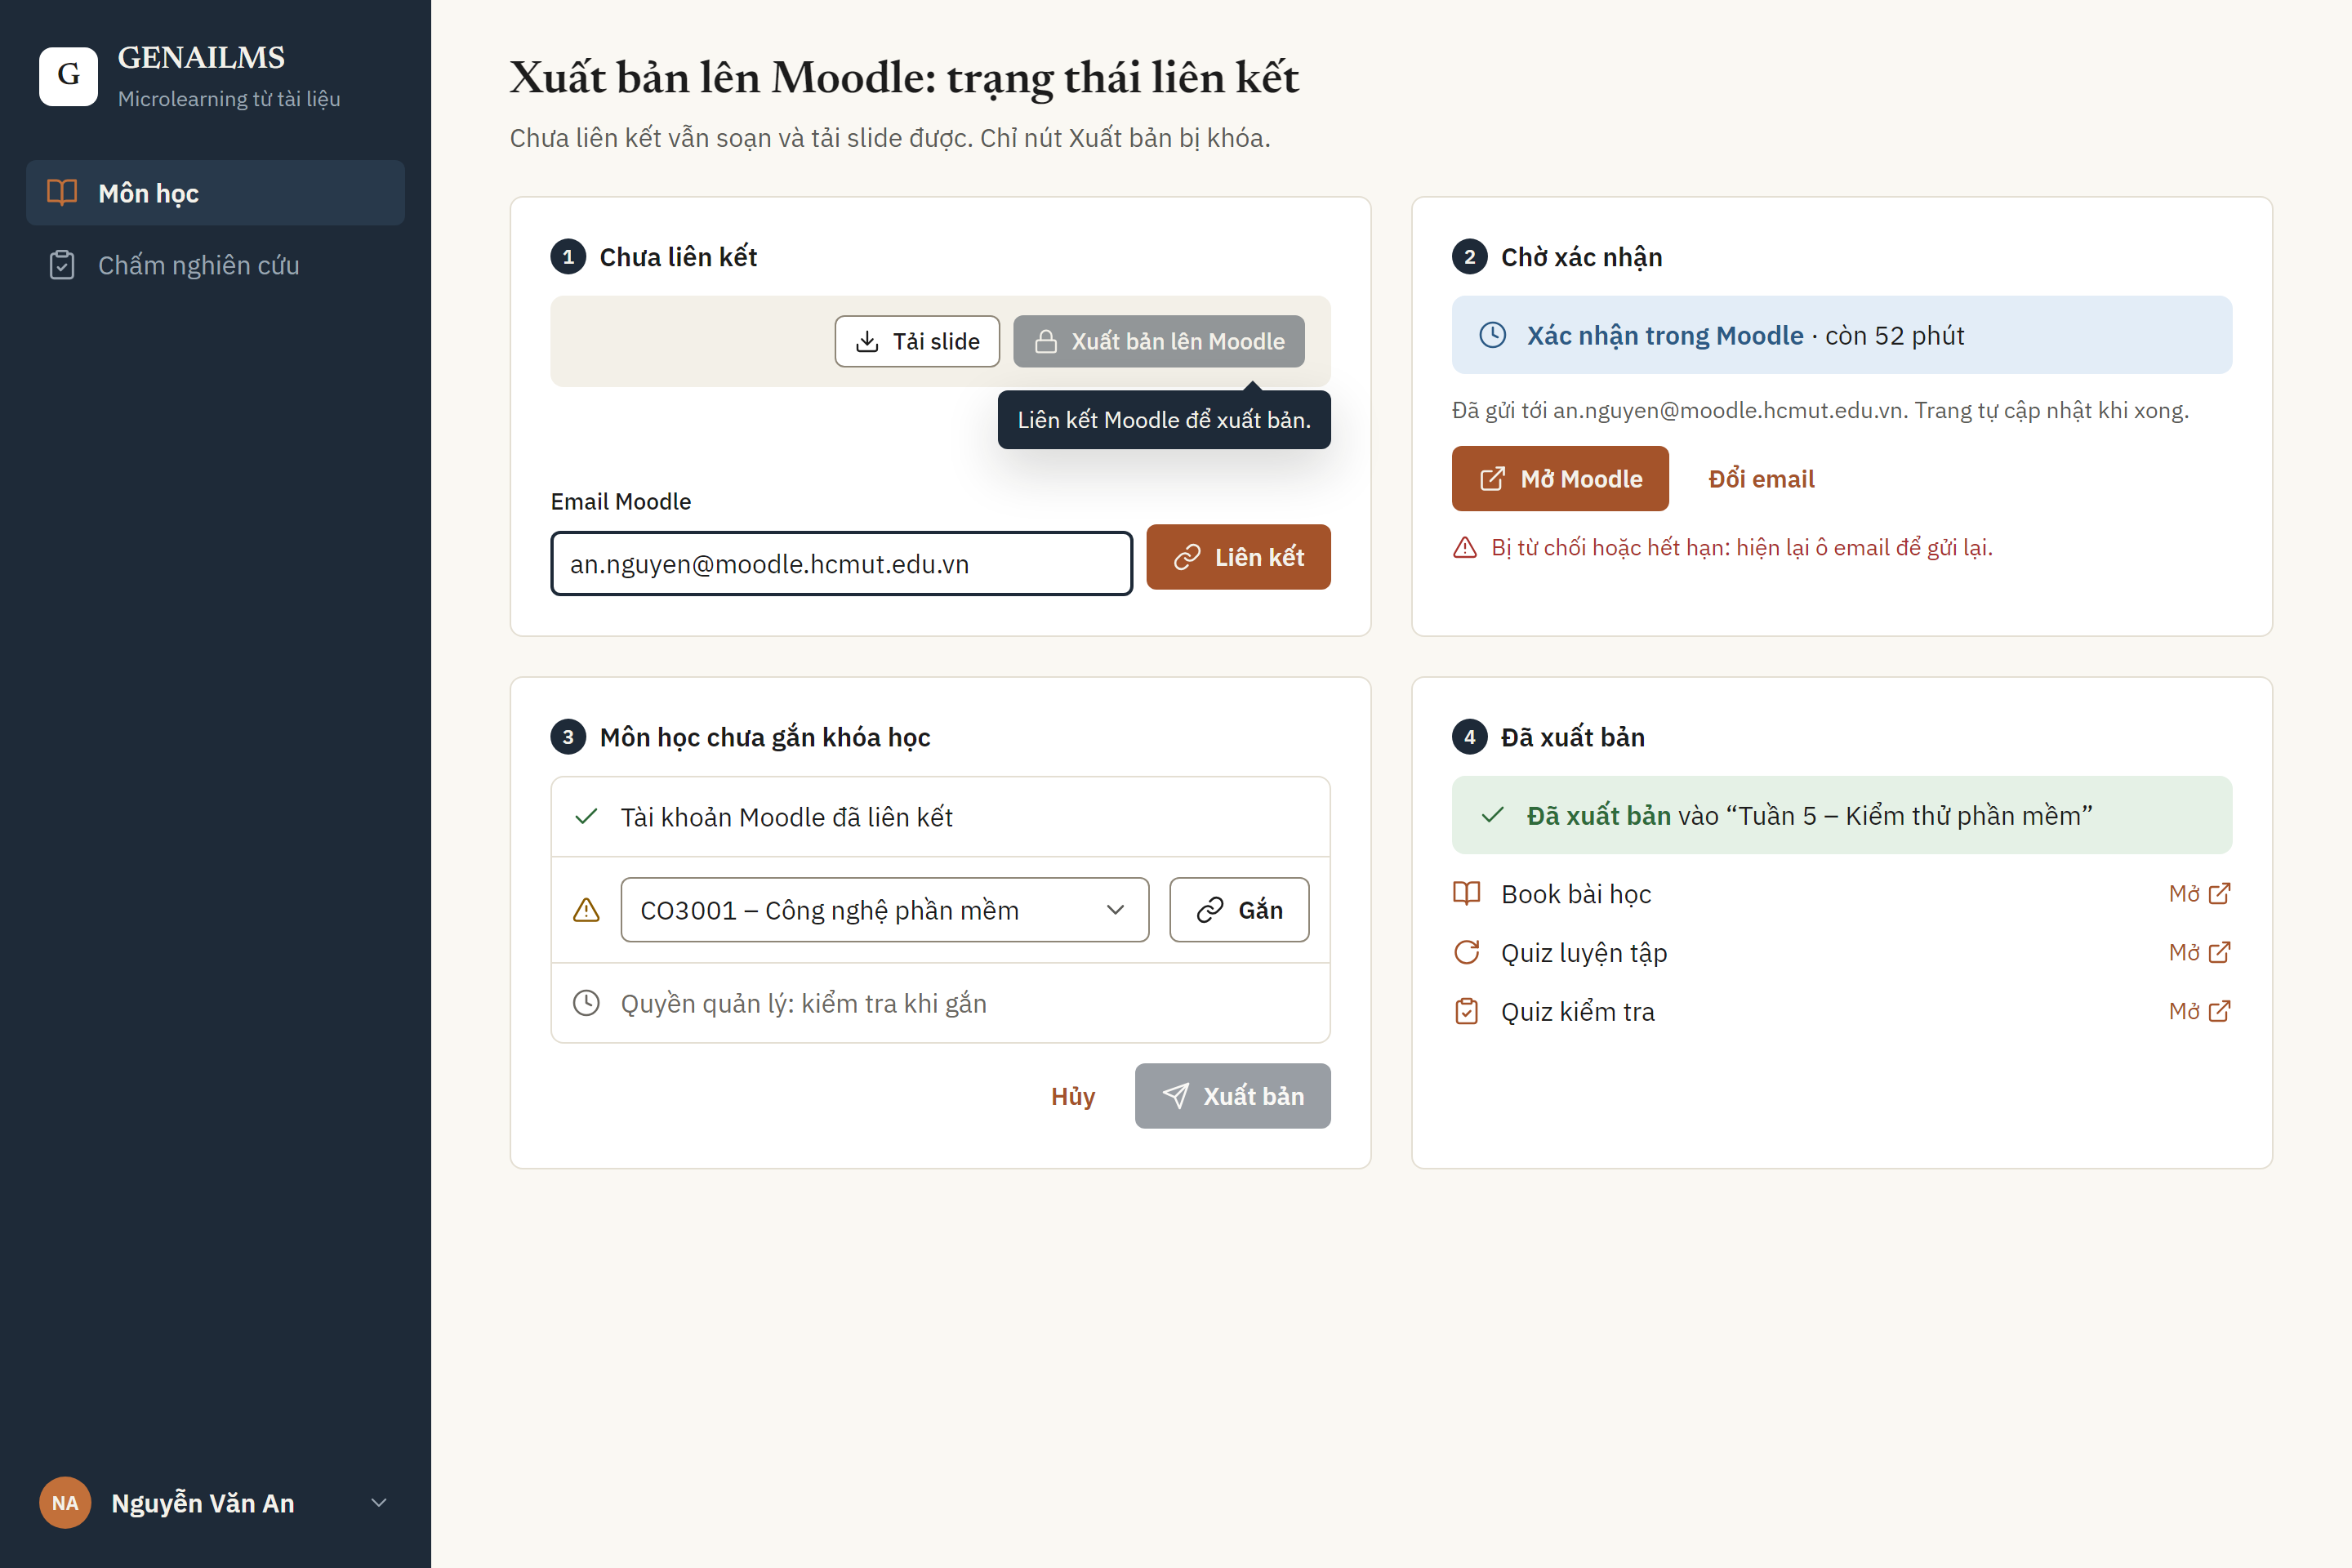
\includegraphics[width=\linewidth,height=.34\textheight,keepaspectratio,viewport={1710 1120 2810 1700},clip]{graphics/ui/09-publish-moodle-link-states.png}
\caption{Pending Moodle confirmation and next actions.}\label{fig:ui-screen-09}
\end{figure}

\needspace{.42\textheight}
The row menu in Figure~\ref{fig:ui-screen-10} groups account actions by the selected person. ``Đặt lại mật khẩu'' means ``Reset password'' and ``Vô hiệu hóa'' means ``Disable''; administrator status does not grant general access to the person's teaching content.
\begin{figure}[H]\centering
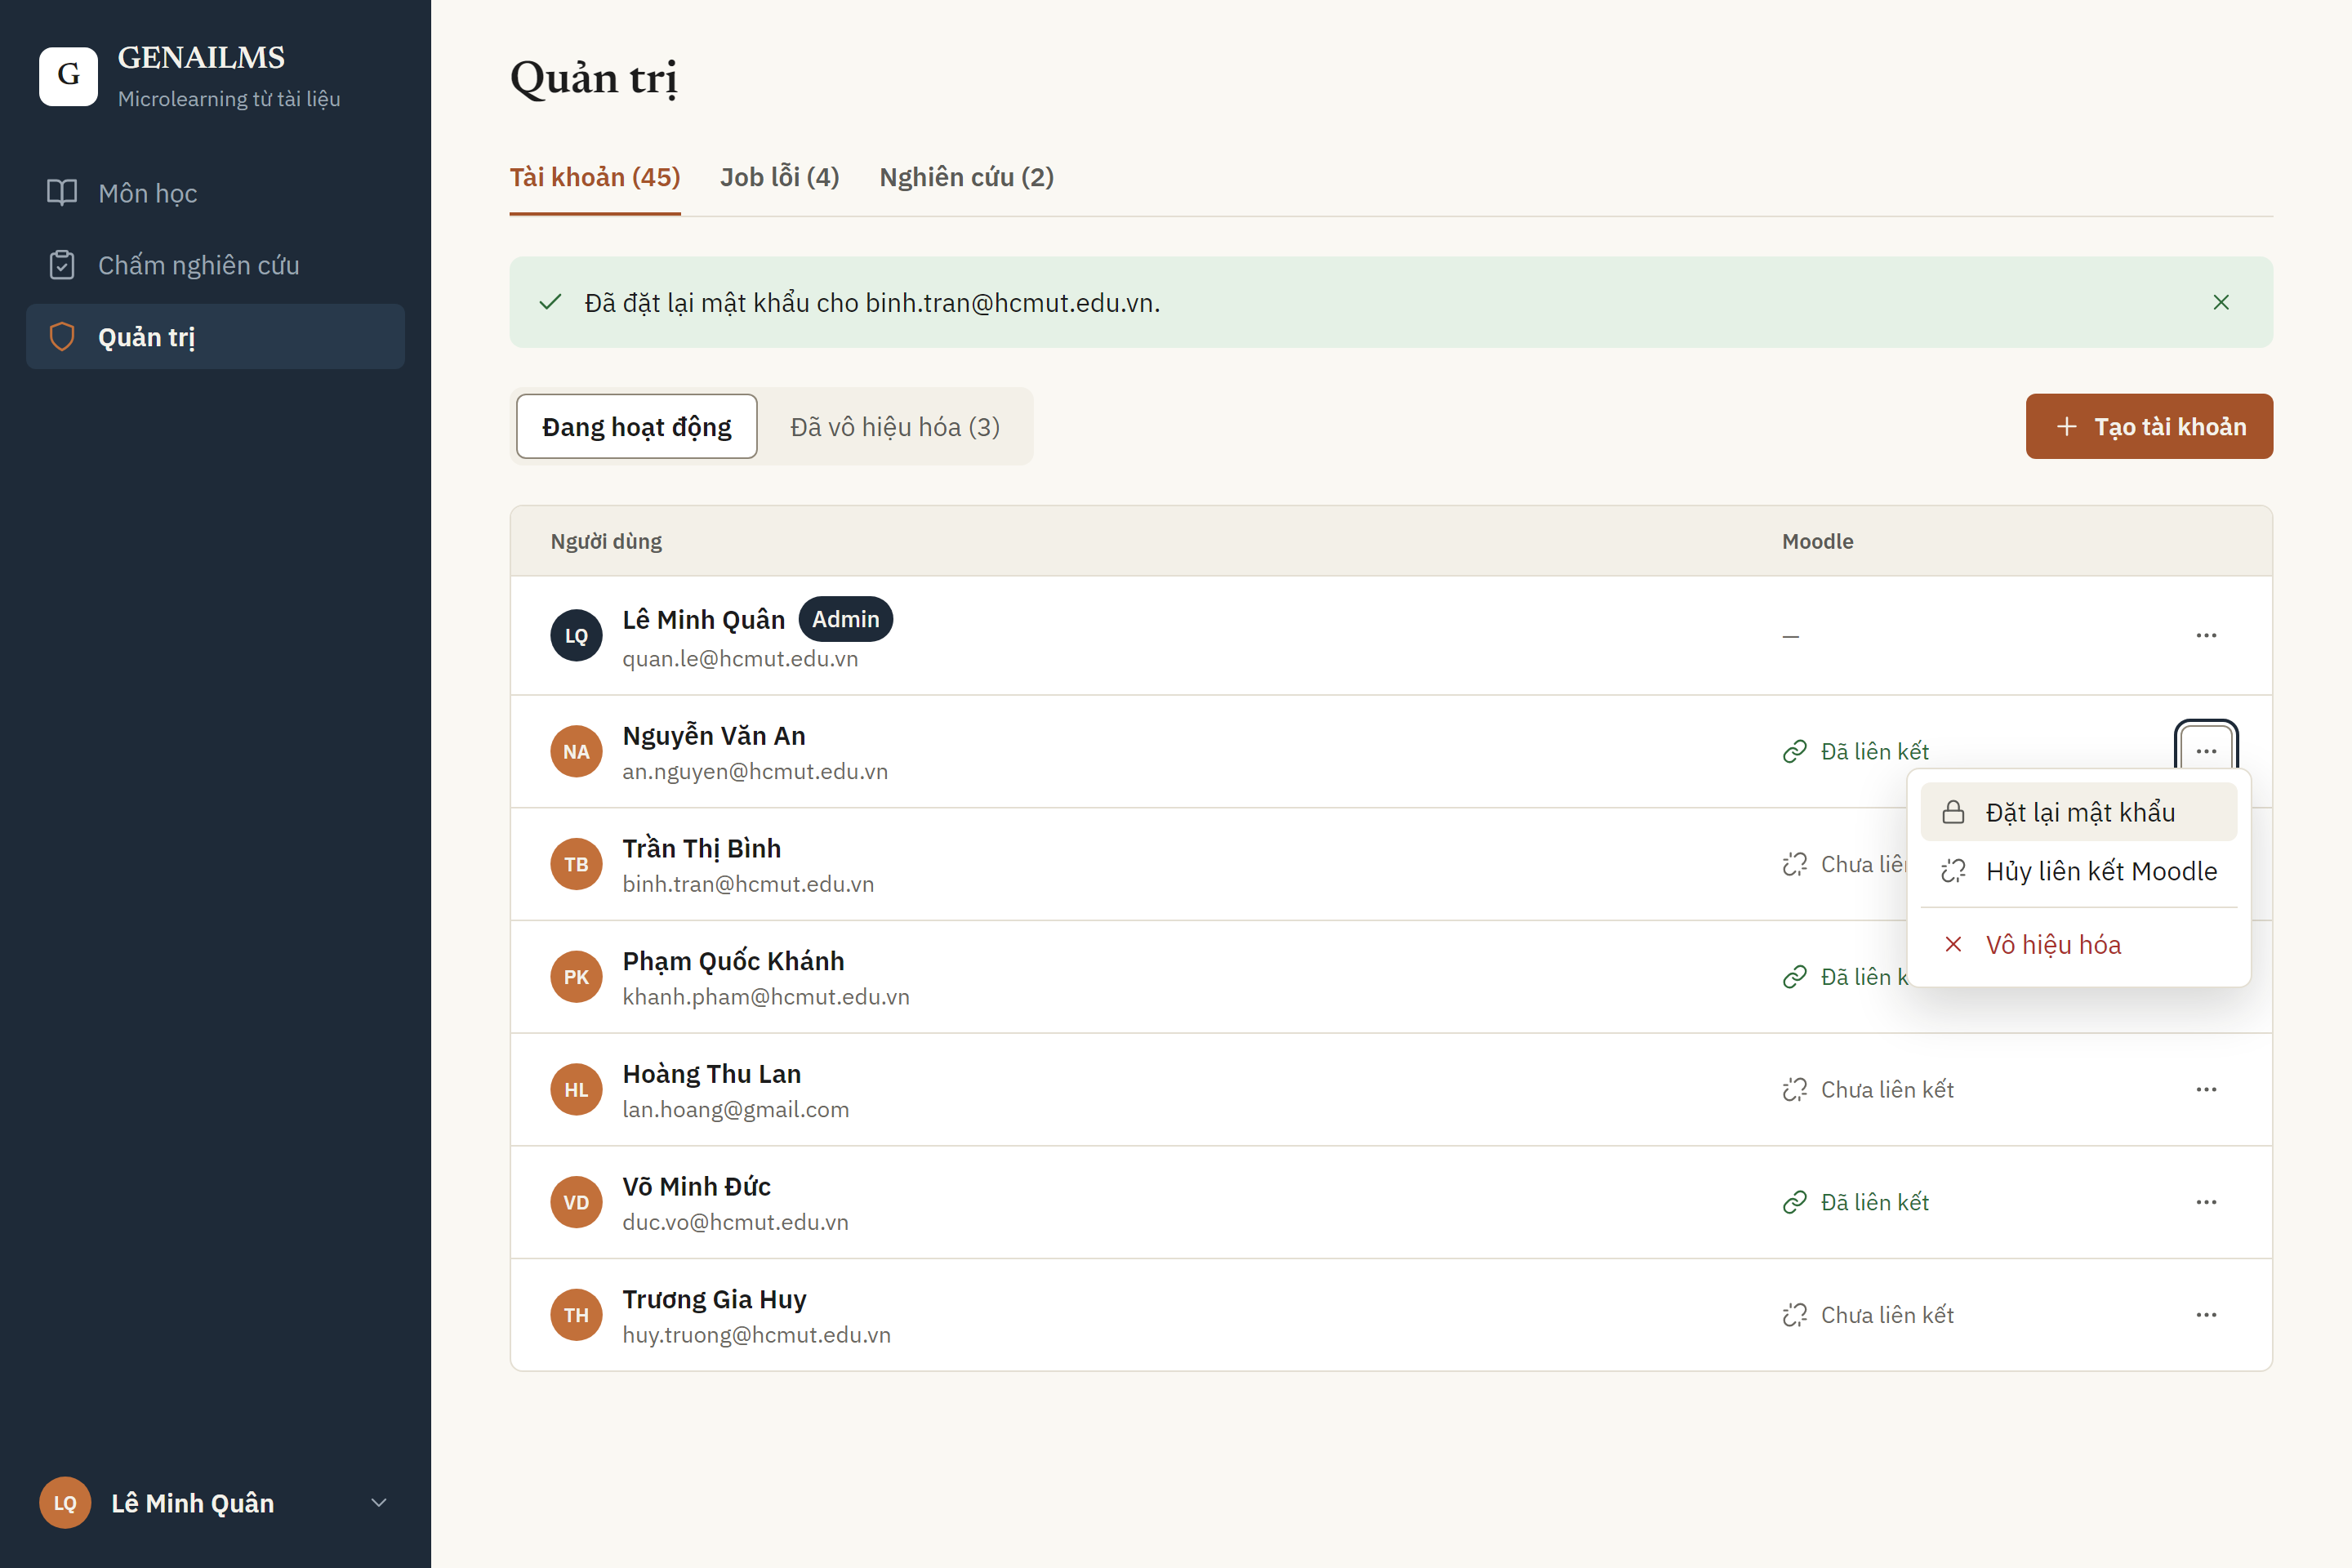
\includegraphics[width=\linewidth,height=.34\textheight,keepaspectratio,viewport={1900 650 2820 1450},clip]{graphics/ui/10-admin-accounts.png}
\caption{Contextual account-administration actions.}\label{fig:ui-screen-10}
\end{figure}

\needspace{.42\textheight}
Figure~\ref{fig:ui-screen-11} exposes failure detail and the permitted retry action. ``Thử lại'' means ``Retry''; the interface distinguishes an author's own job from the administrator's operational recovery scope.
\begin{figure}[H]\centering
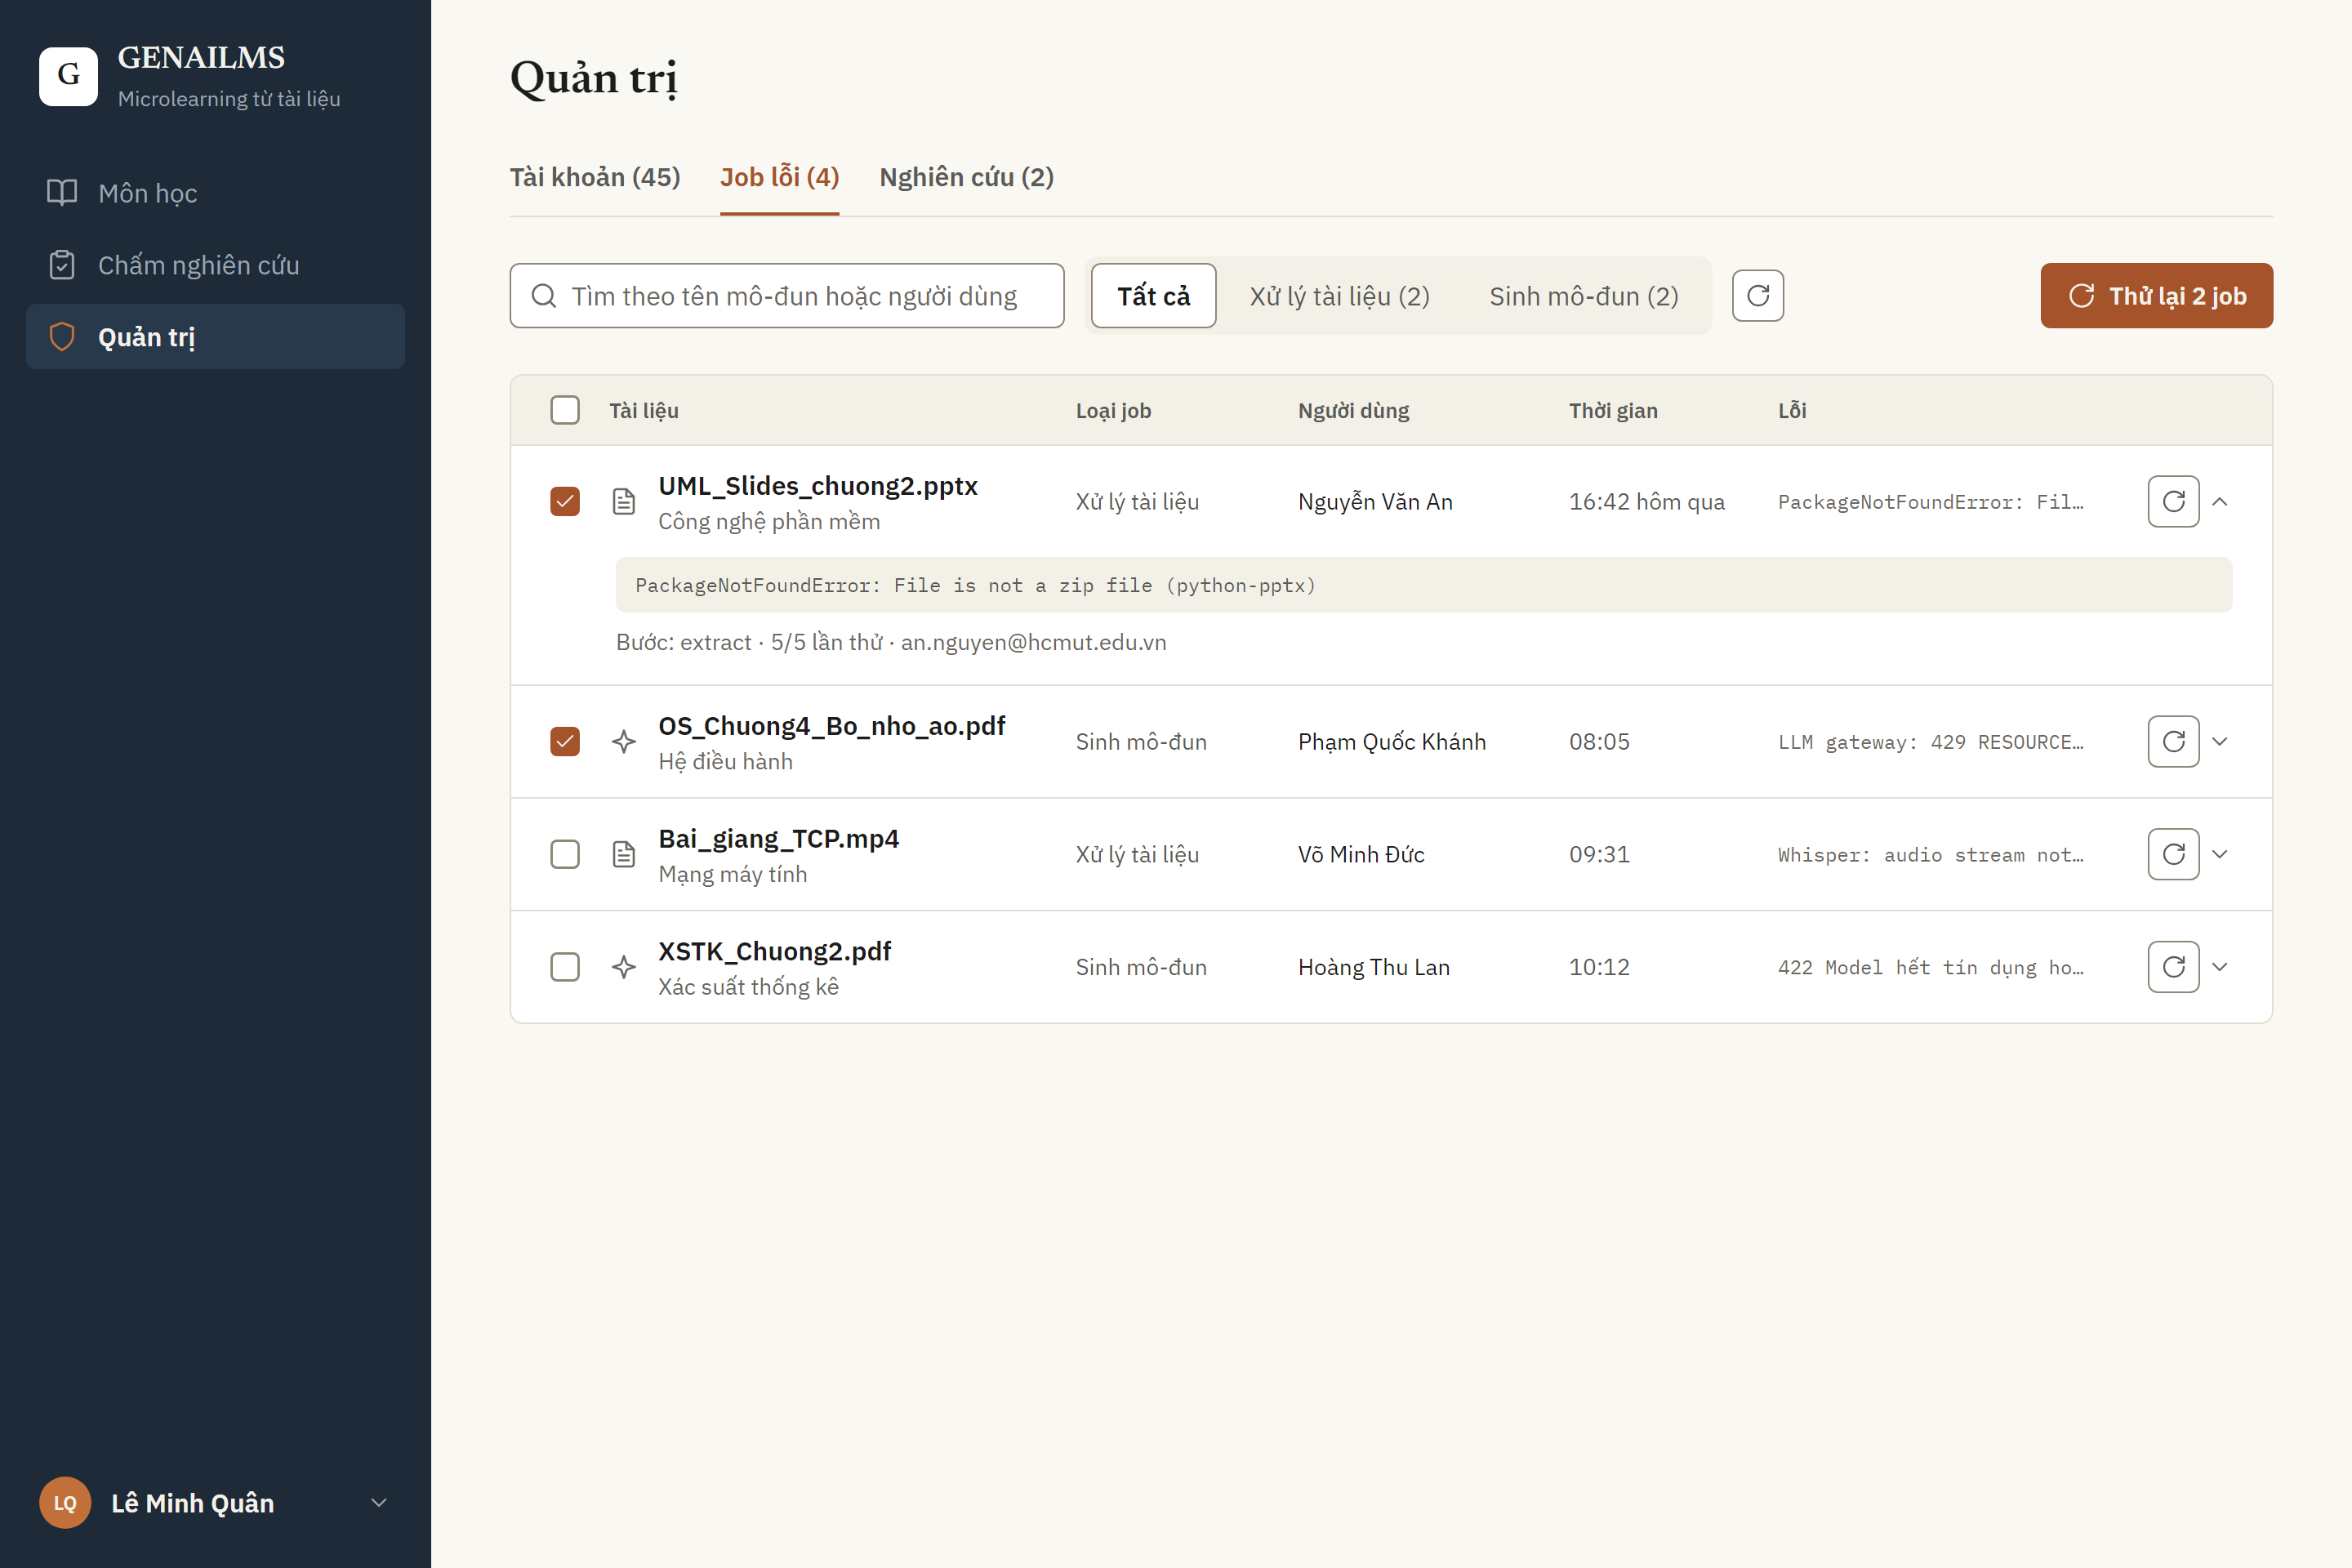
\includegraphics[width=\linewidth,height=.34\textheight,keepaspectratio,viewport={1200 850 2820 1550},clip]{graphics/ui/11-admin-failed-jobs.png}
\caption{Failed-job inspection and recovery.}\label{fig:ui-screen-11}
\end{figure}

\needspace{.42\textheight}
Figure~\ref{fig:ui-screen-12} groups study identity, snapshot preparation and rater invitations in an administrative workspace. ``Nghiên cứu'' means ``Study''; anonymous packet preparation precedes activation for raters.
\begin{figure}[H]\centering
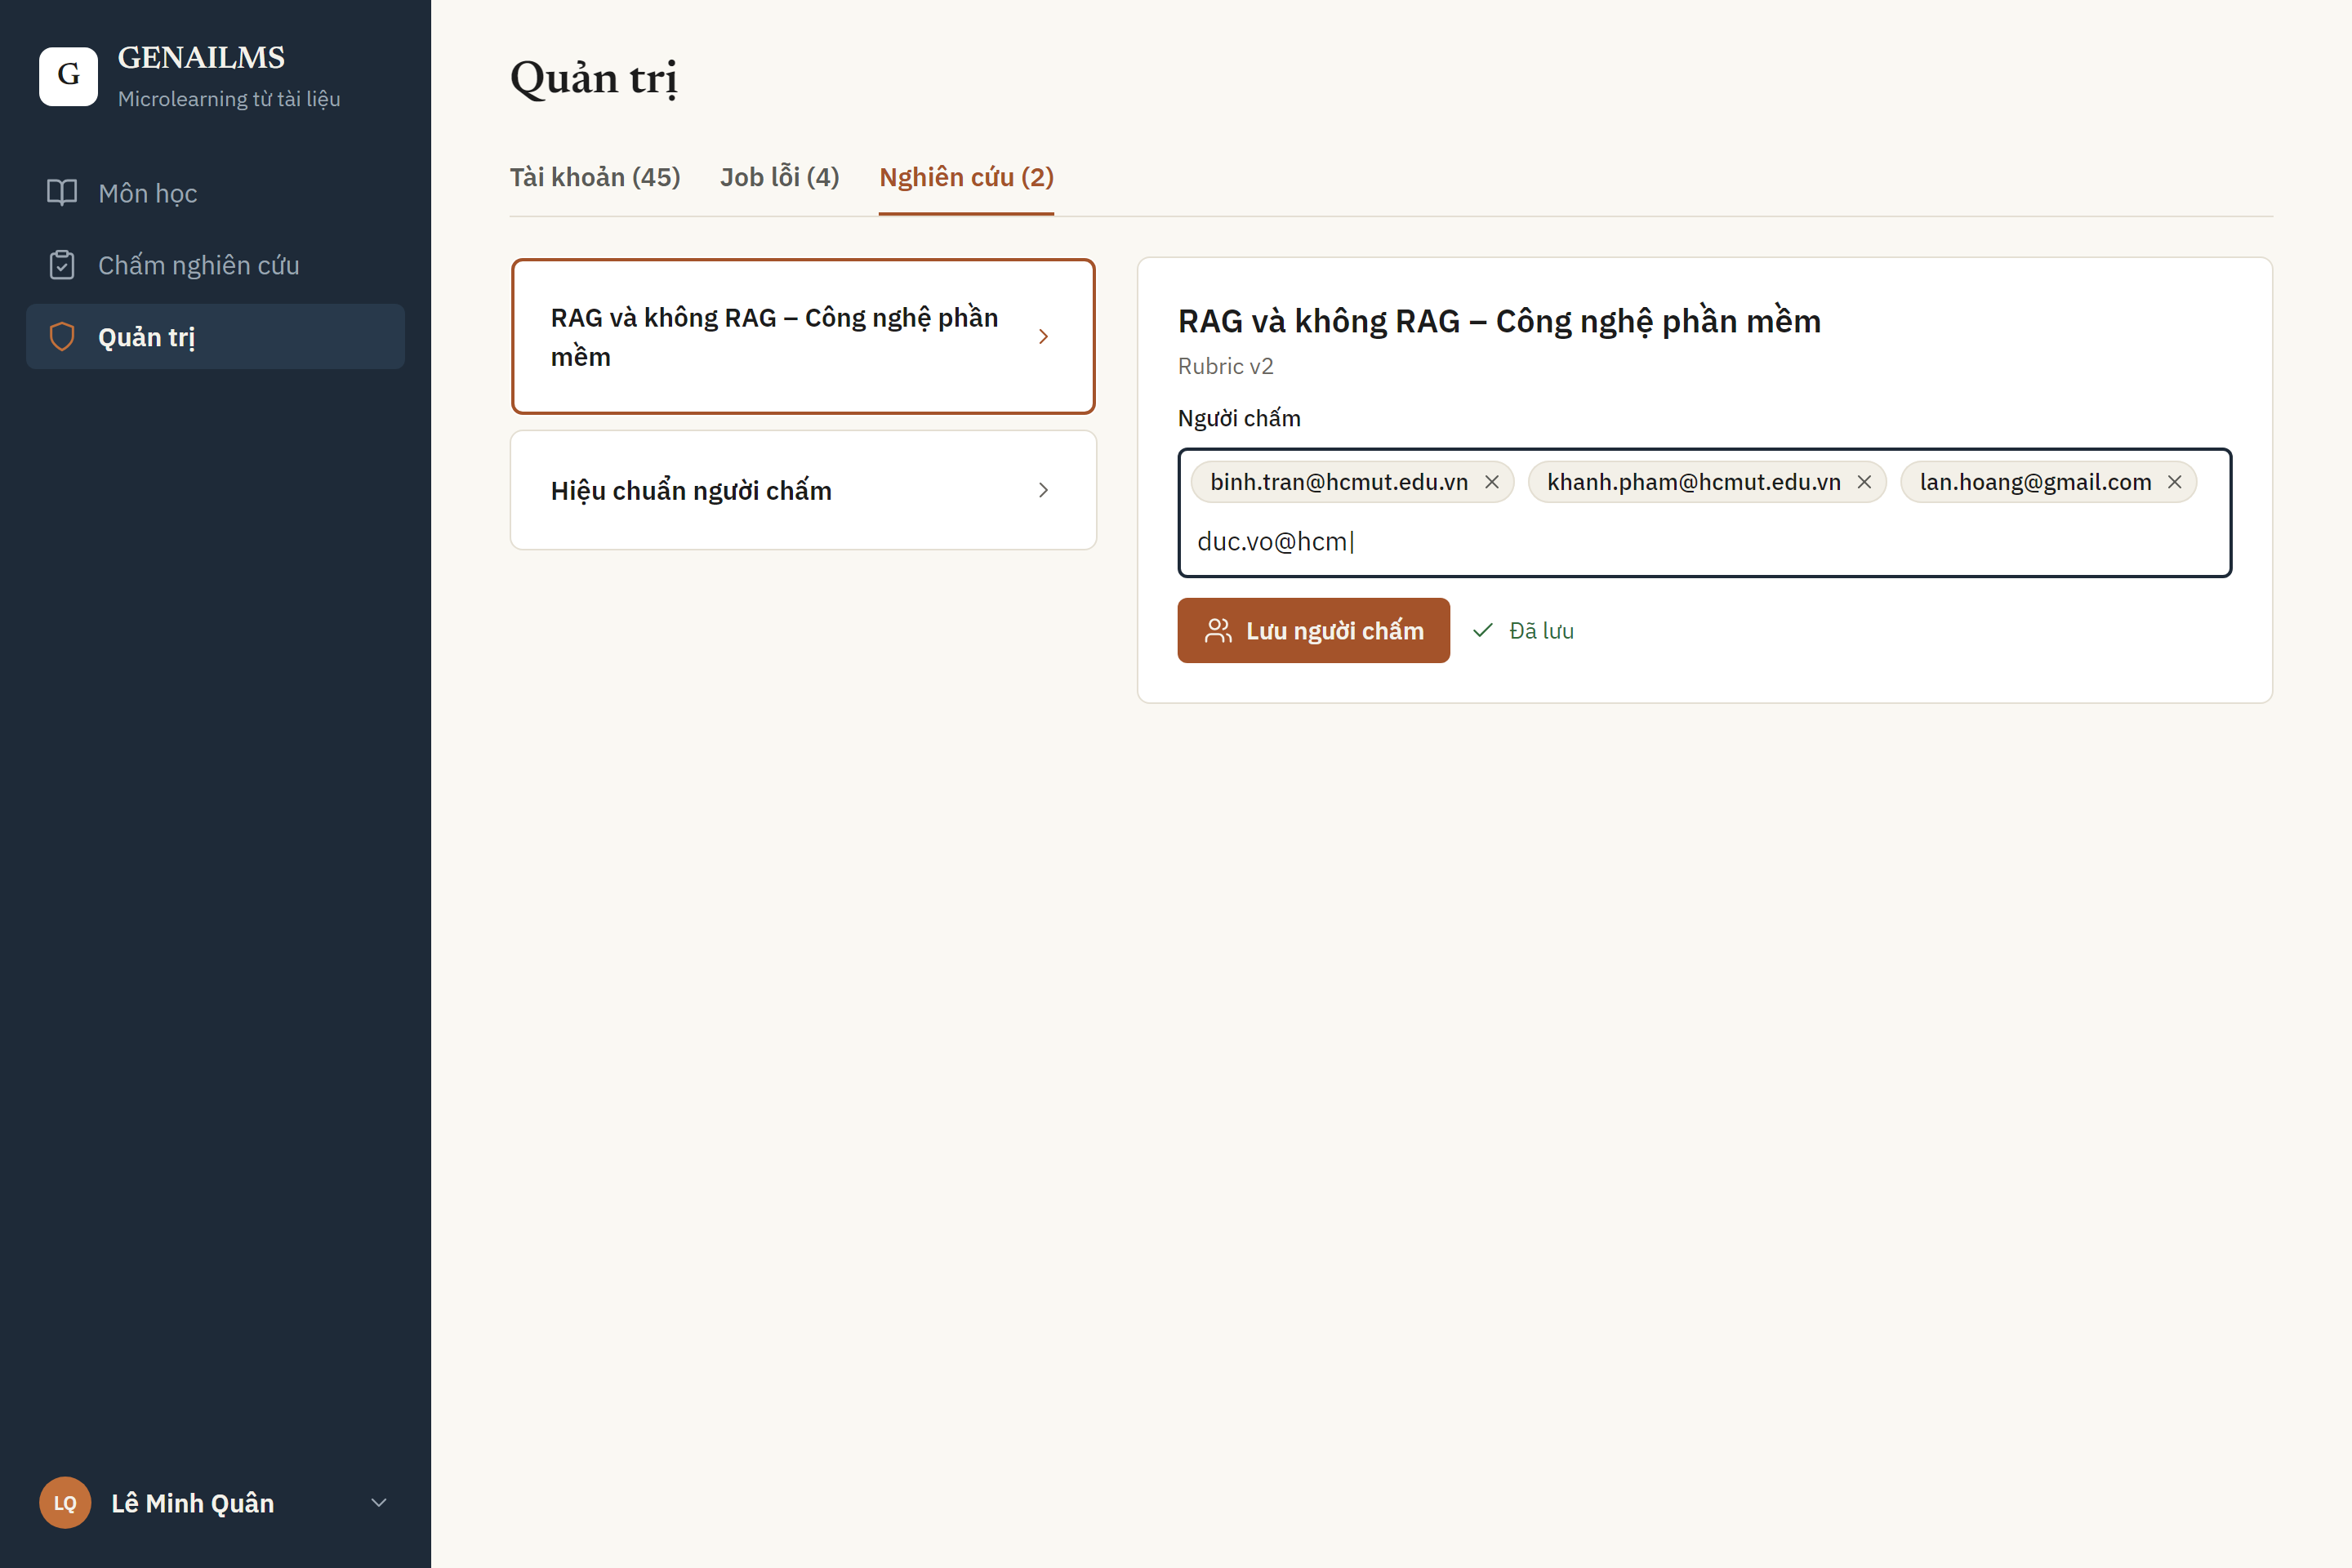
\includegraphics[width=\linewidth,height=.34\textheight,keepaspectratio,viewport={1370 1030 2810 1630},clip]{graphics/ui/12-admin-studies.png}
\caption{Study preparation and invitations.}\label{fig:ui-screen-12}
\end{figure}

\needspace{.42\textheight}
Figure~\ref{fig:ui-screen-13} enlarges the scoring controls and the reason field in the blinded-rating screen. ``Nhận xét'' means ``Comment''; the 1--5 controls and written reasons are recorded per criterion while the packet order remains stable for the rater.
\begin{figure}[H]\centering
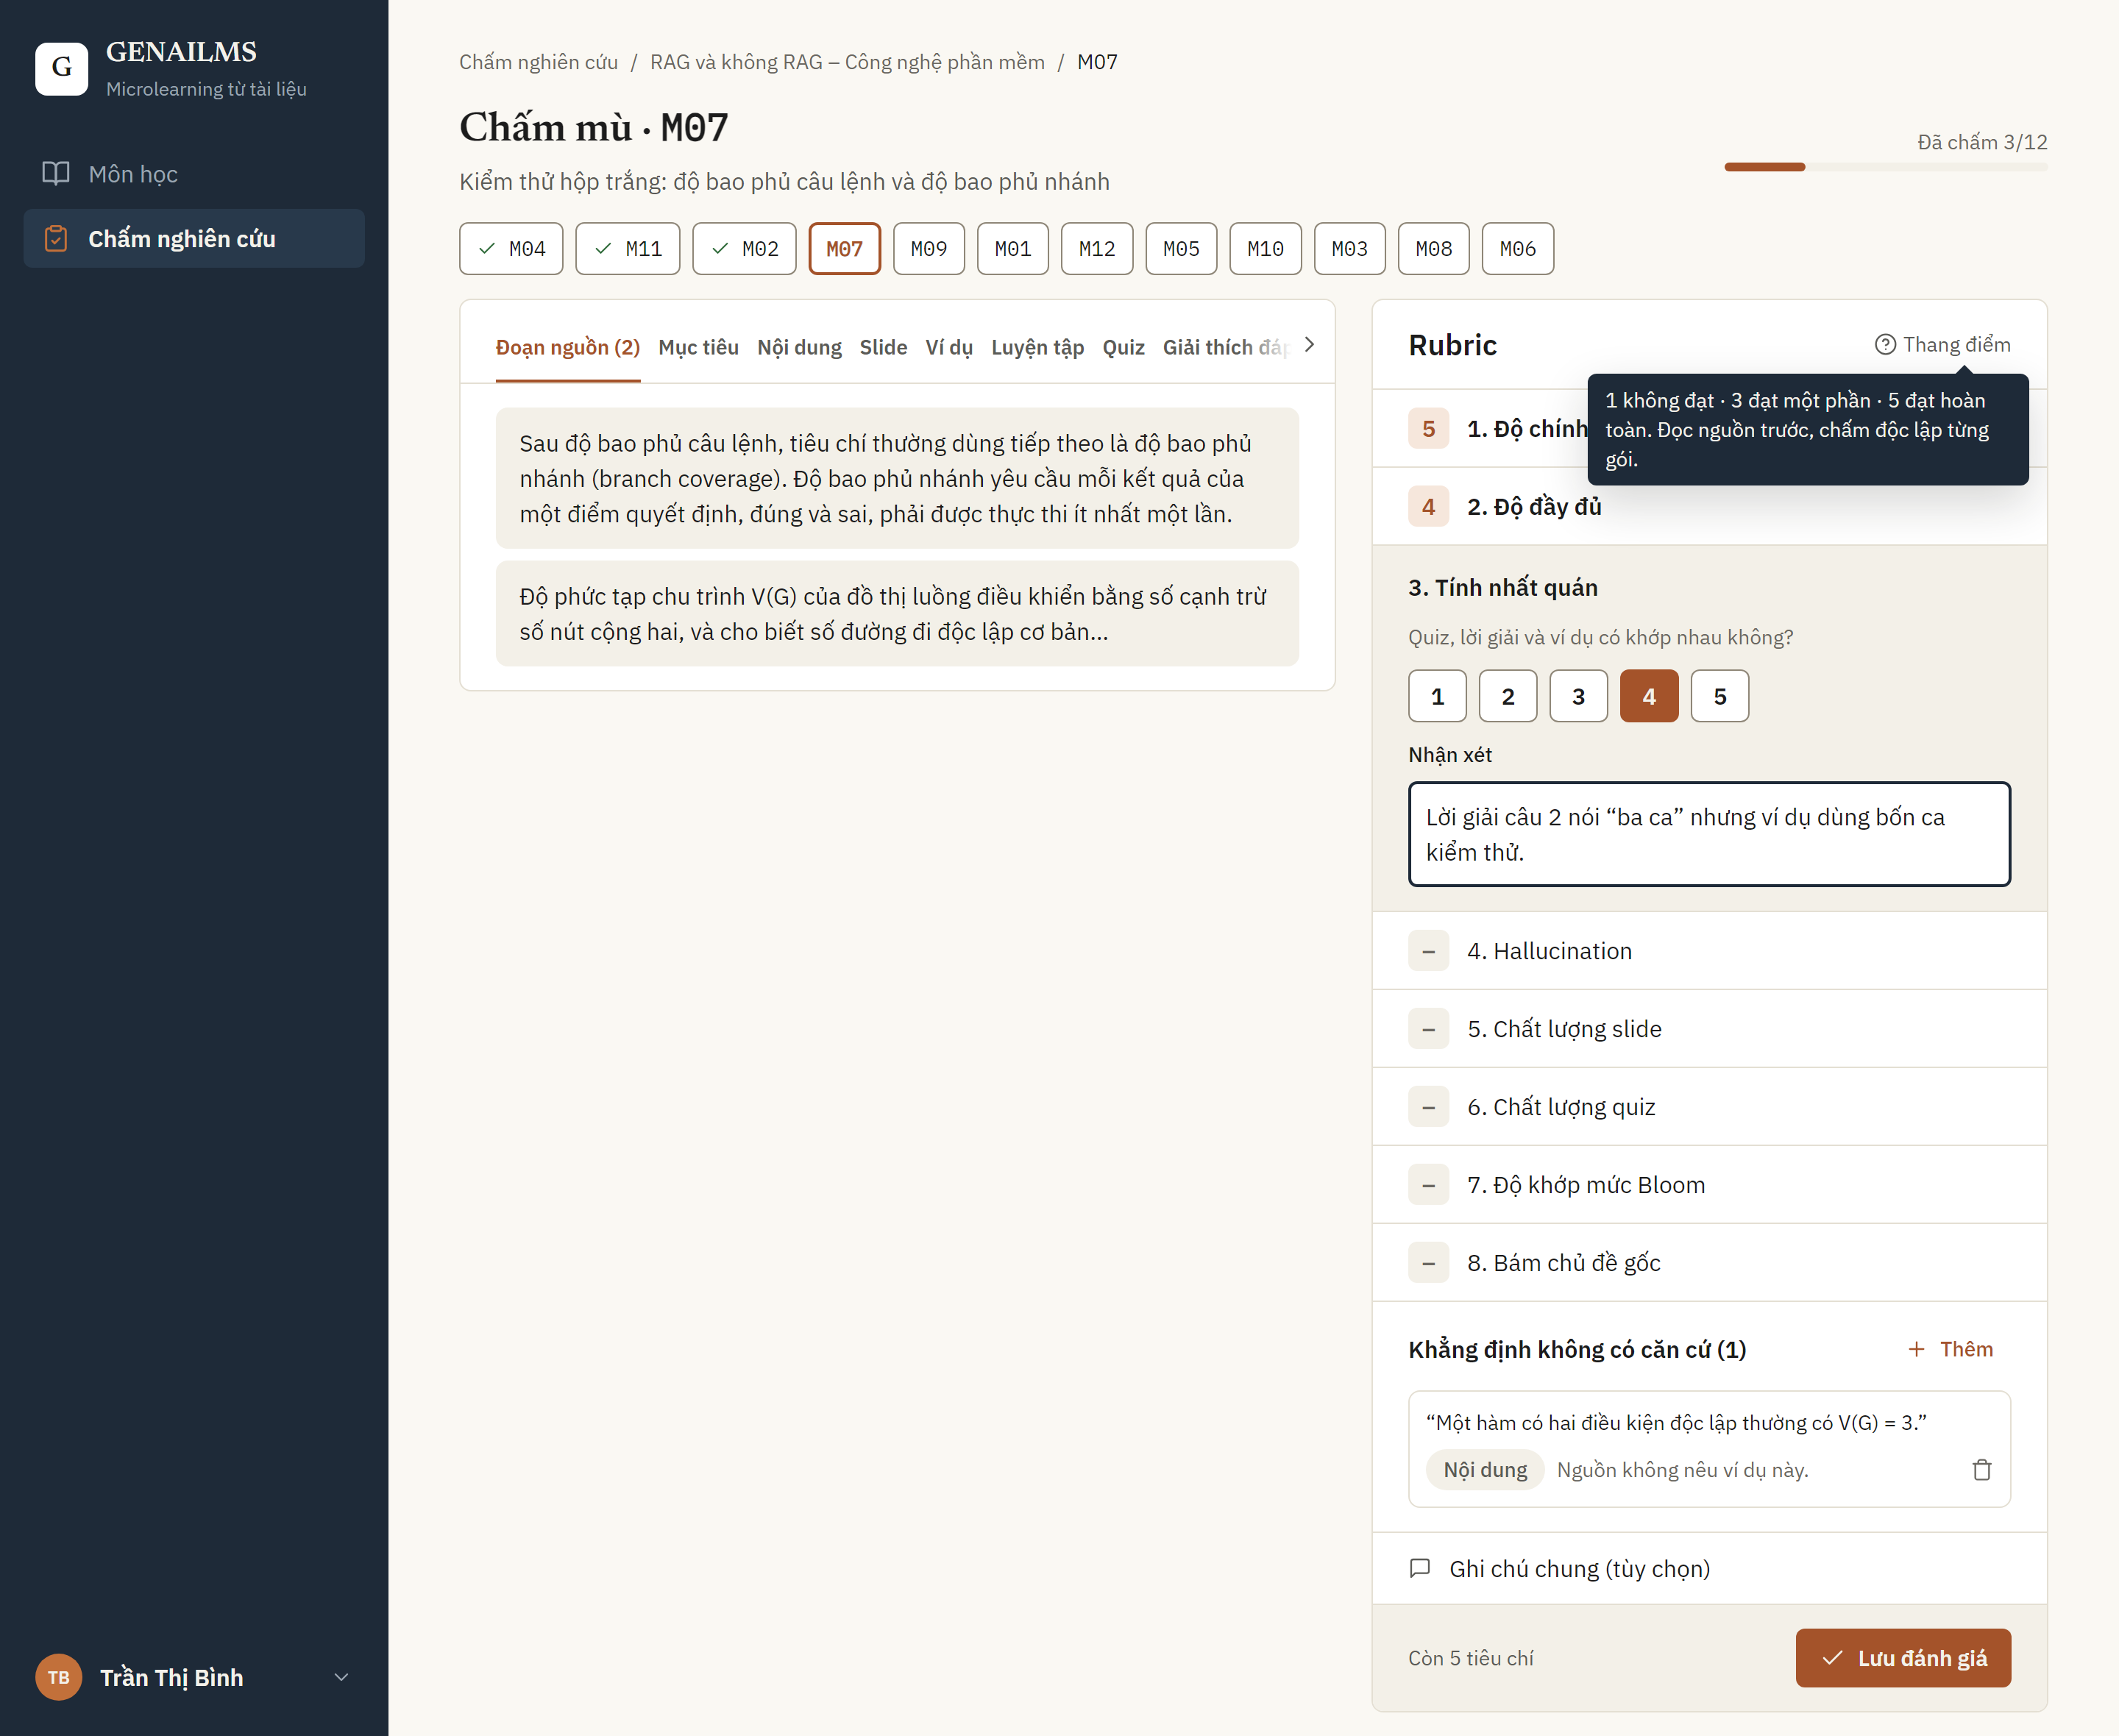
\includegraphics[width=\linewidth,height=.34\textheight,keepaspectratio,viewport={1850 1100 2800 1580},clip]{graphics/ui/13-rater-blind-rating.png}
\caption{Focused rubric and criterion-level reasoning.}\label{fig:ui-screen-13}
\end{figure}

\needspace{.42\textheight}
Figure~\ref{fig:ui-screen-14} shows the course workspace as a single column on a mobile viewport. Upload, status and generation actions retain text labels; secondary information collapses without hiding failure recovery.
\begin{figure}[H]\centering
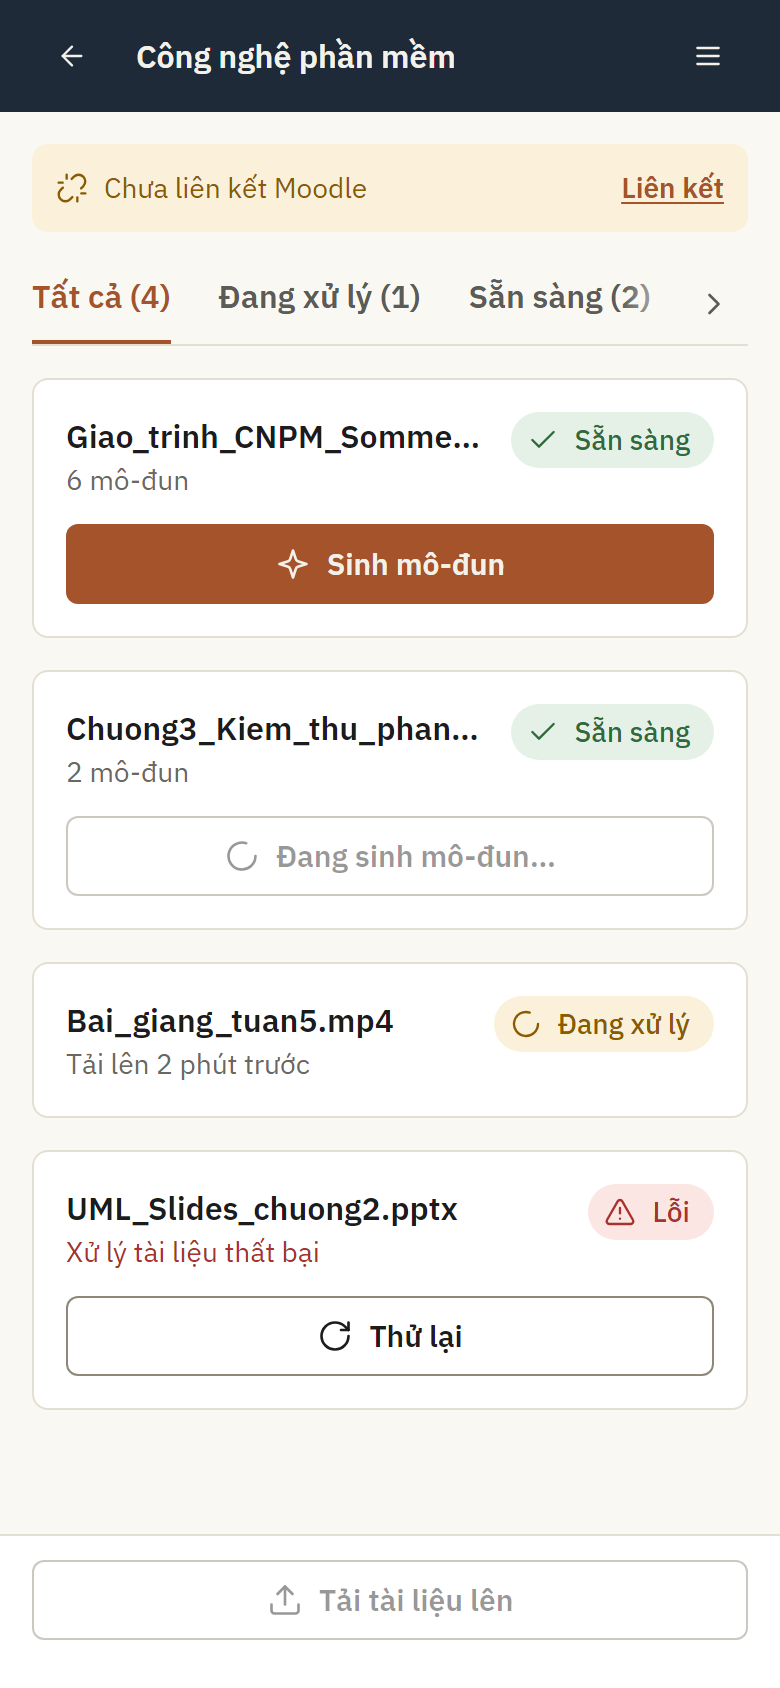
\includegraphics[width=.65\linewidth,height=.60\textheight,keepaspectratio]{graphics/ui/14-mobile-course-detail.png}
\caption{Mobile authoring workspace.}\label{fig:ui-screen-14}
\end{figure}

\needspace{.42\textheight}
Figure~\ref{fig:ui-screen-15} shows empty-course, empty-document and loading panels. ``Chưa có môn học'' means ``No courses yet'' and ``Chọn tệp'' means ``Choose file''; useful next actions appear directly in the empty state.
\begin{figure}[H]\centering
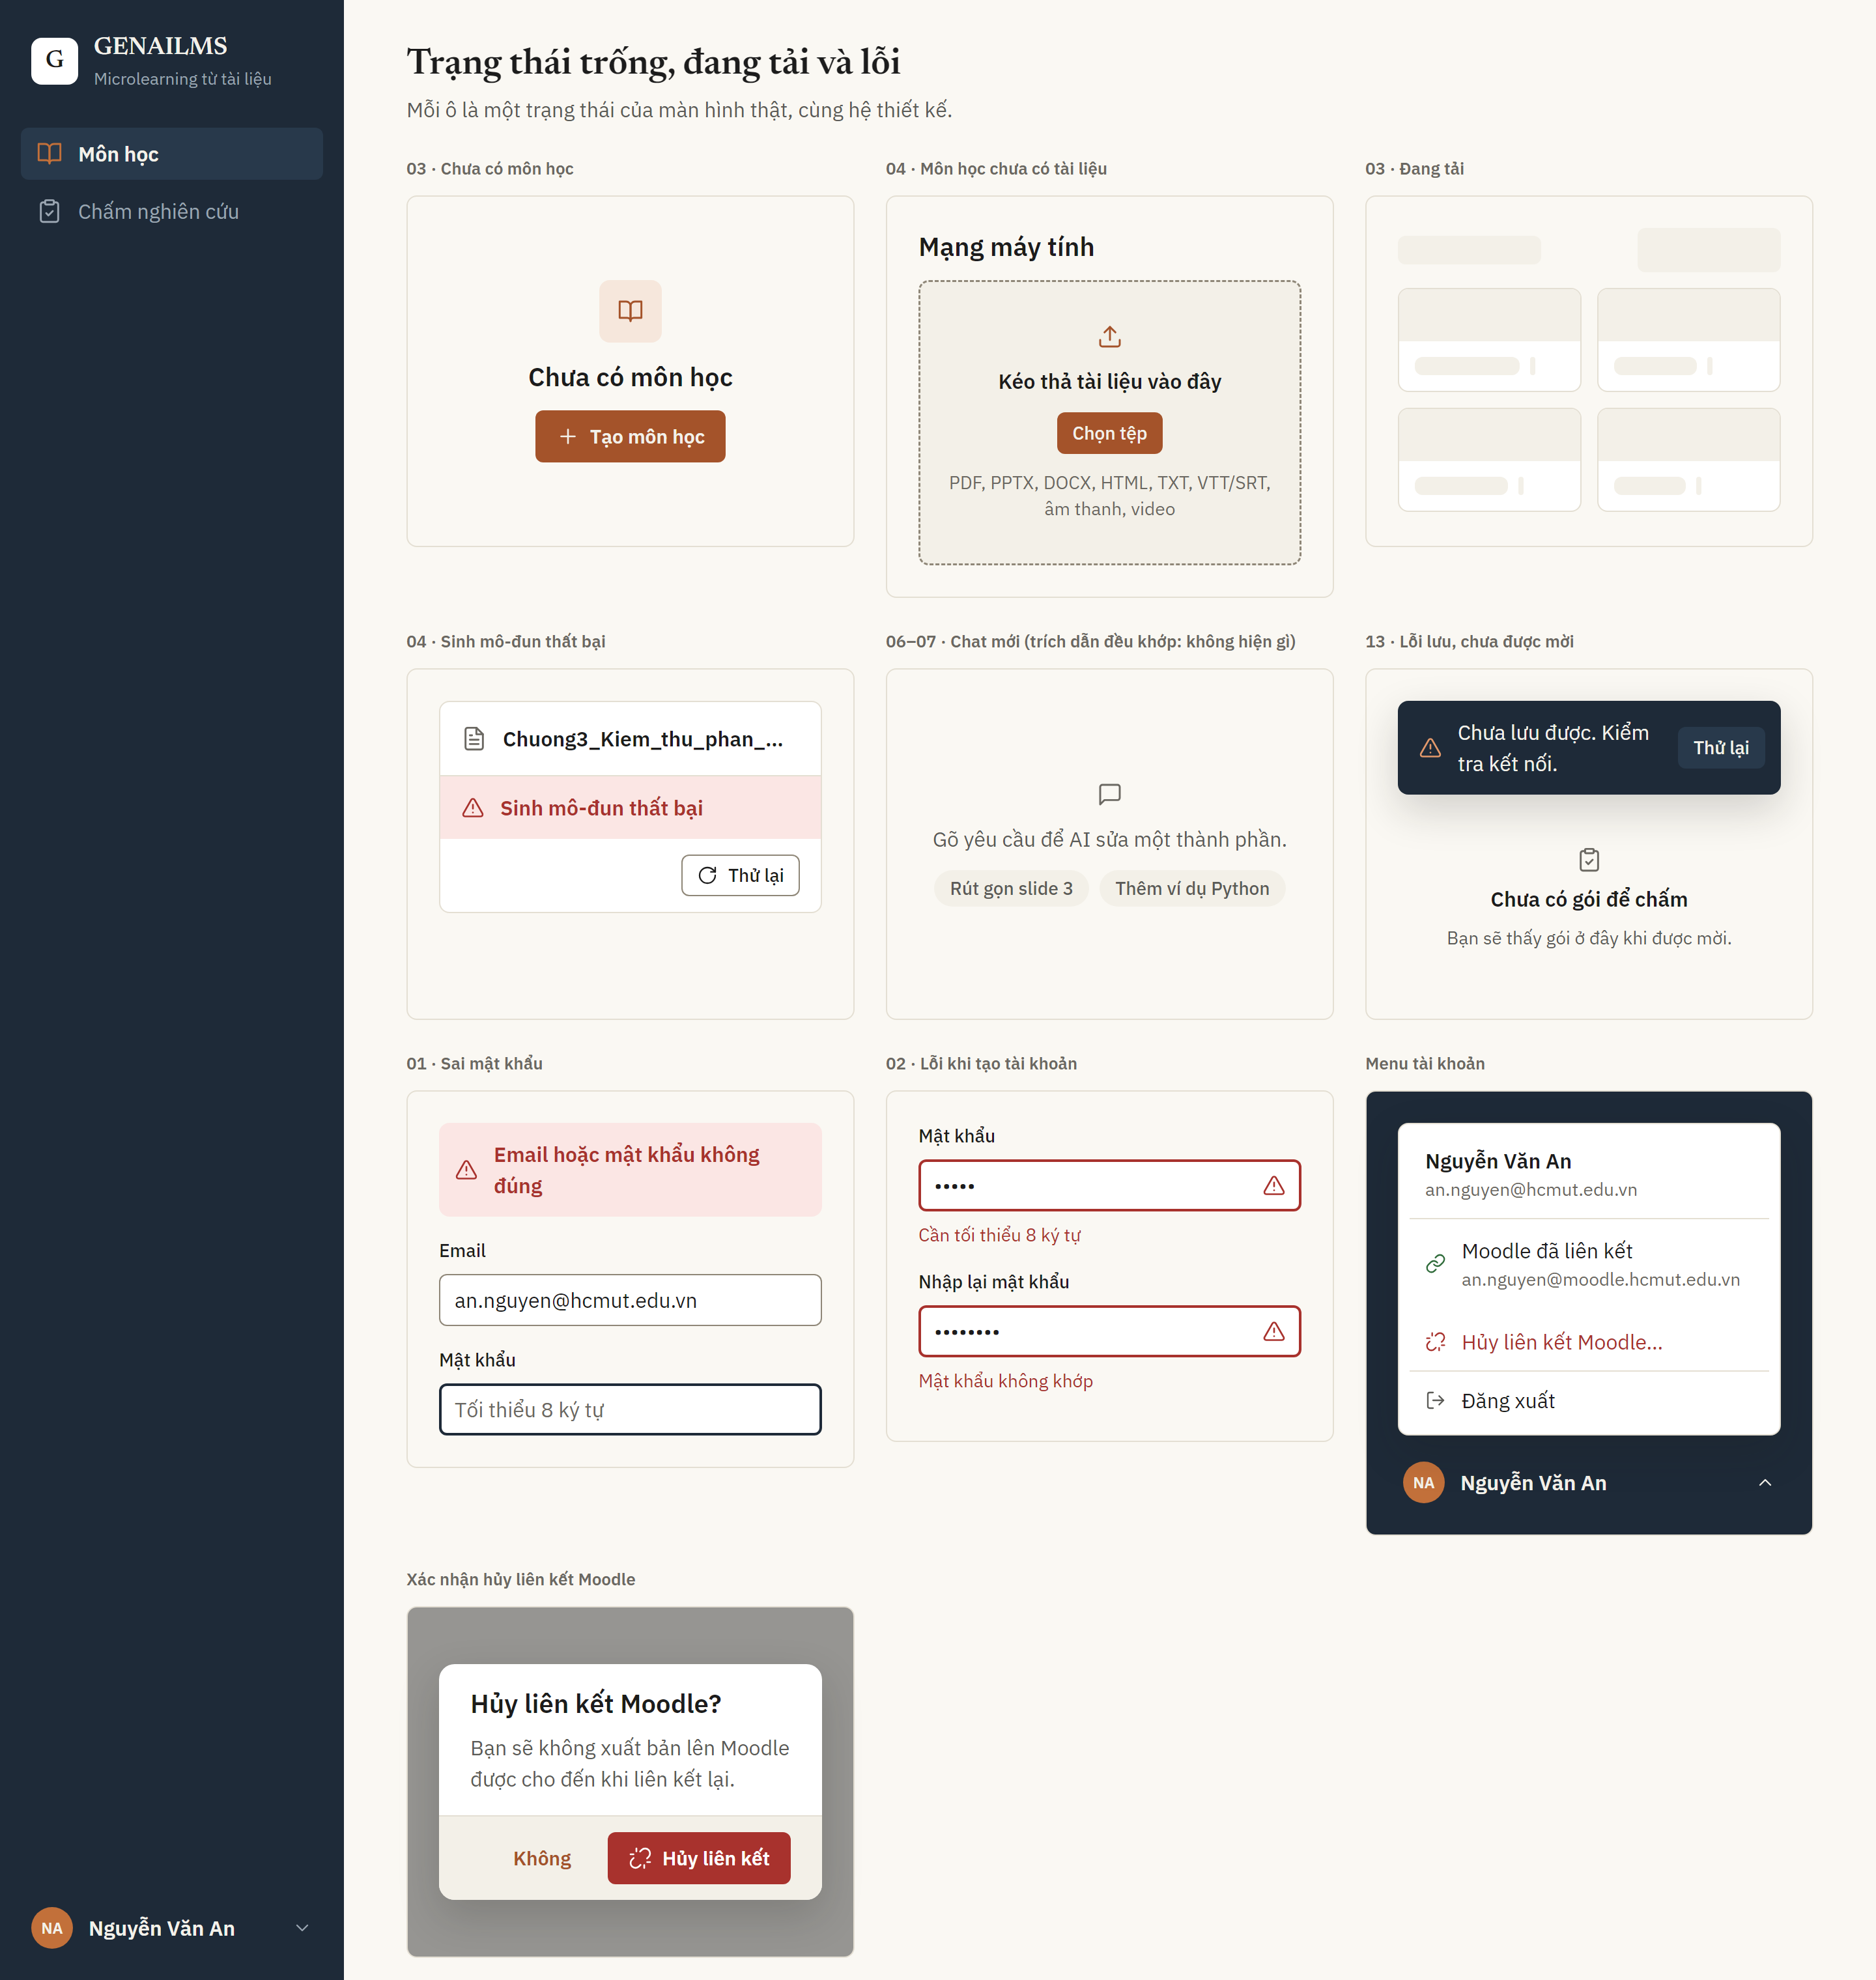
\includegraphics[width=.47\linewidth,height=.26\textheight,keepaspectratio,viewport={620 2200 1320 2750},clip]{graphics/ui/15-empty-loading-error-states.png}\hfill
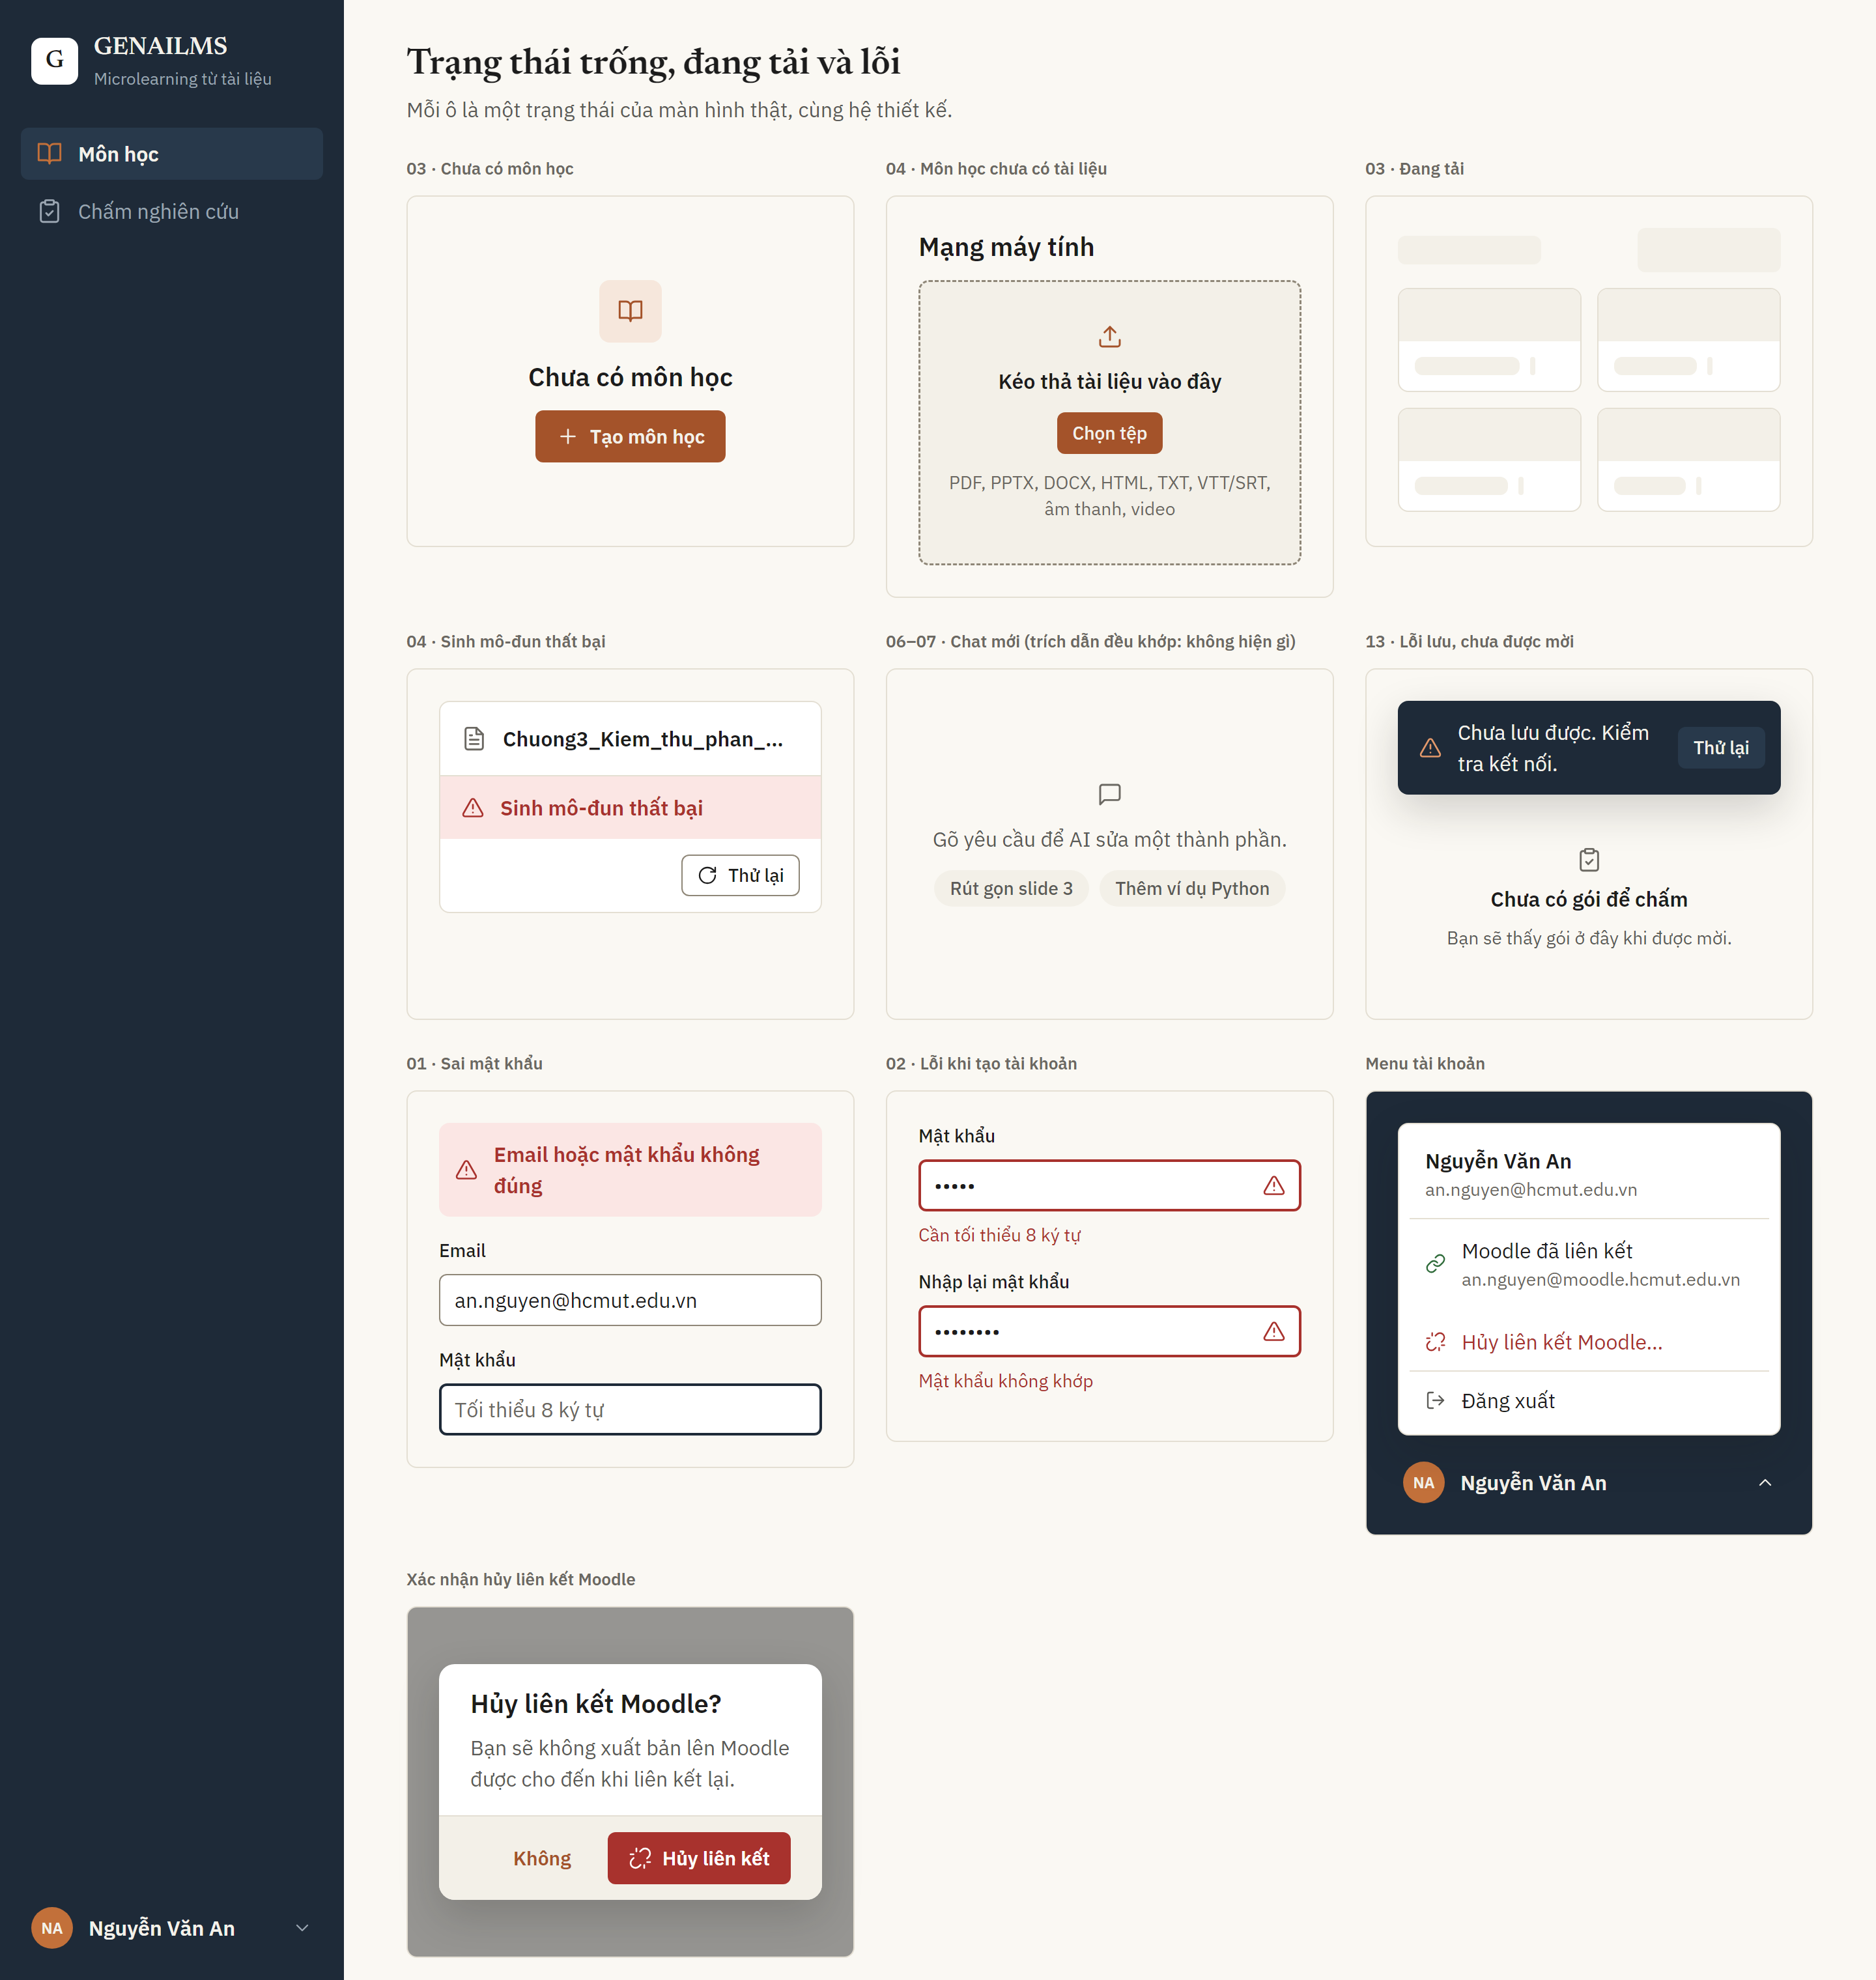
\includegraphics[width=.47\linewidth,height=.26\textheight,keepaspectratio,viewport={1360 2110 2050 2750},clip]{graphics/ui/15-empty-loading-error-states.png}\par\smallskip
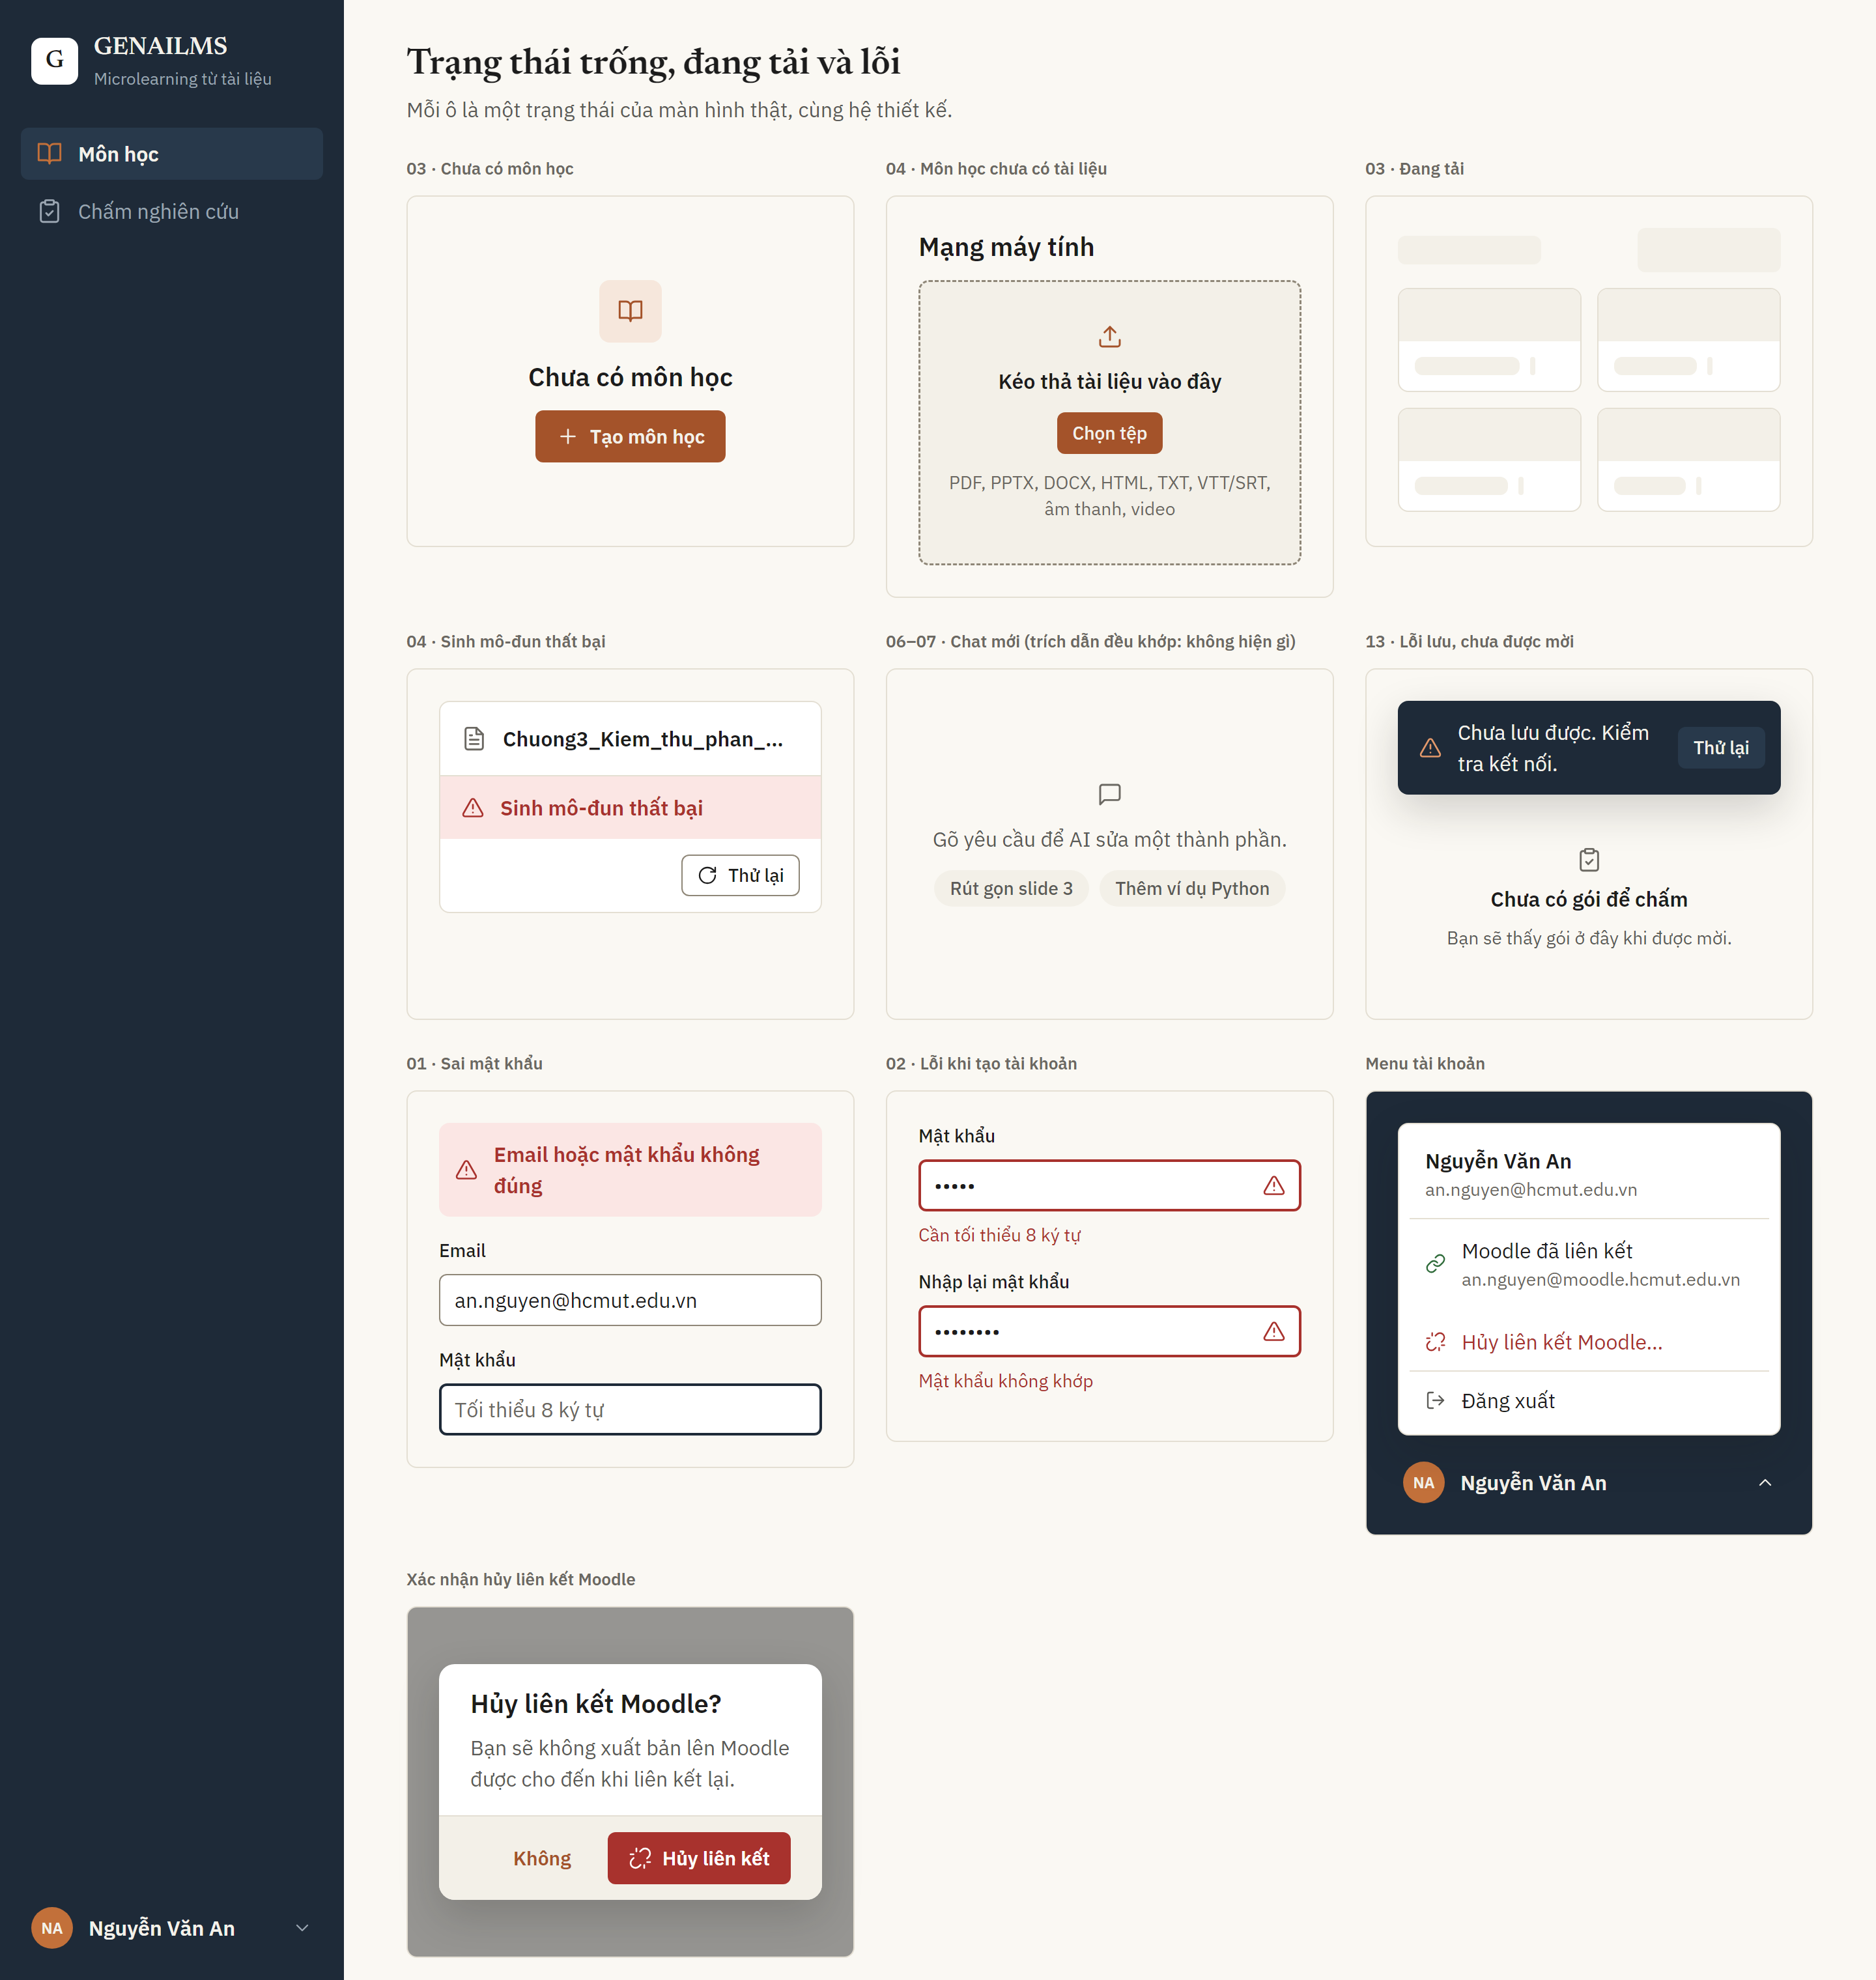
\includegraphics[width=.47\linewidth,height=.26\textheight,keepaspectratio,viewport={2100 2200 2800 2750},clip]{graphics/ui/15-empty-loading-error-states.png}\hfill
\caption{Empty and loading states.}\label{fig:ui-screen-15}
\end{figure}

\needspace{.42\textheight}
Figure~\ref{fig:ui-screen-15-recovery} groups generation failure, an empty editing conversation and a failed rating save. ``Chưa lưu được'' means ``Could not save''; the interface preserves entered work and offers retry.
\begin{figure}[H]\centering
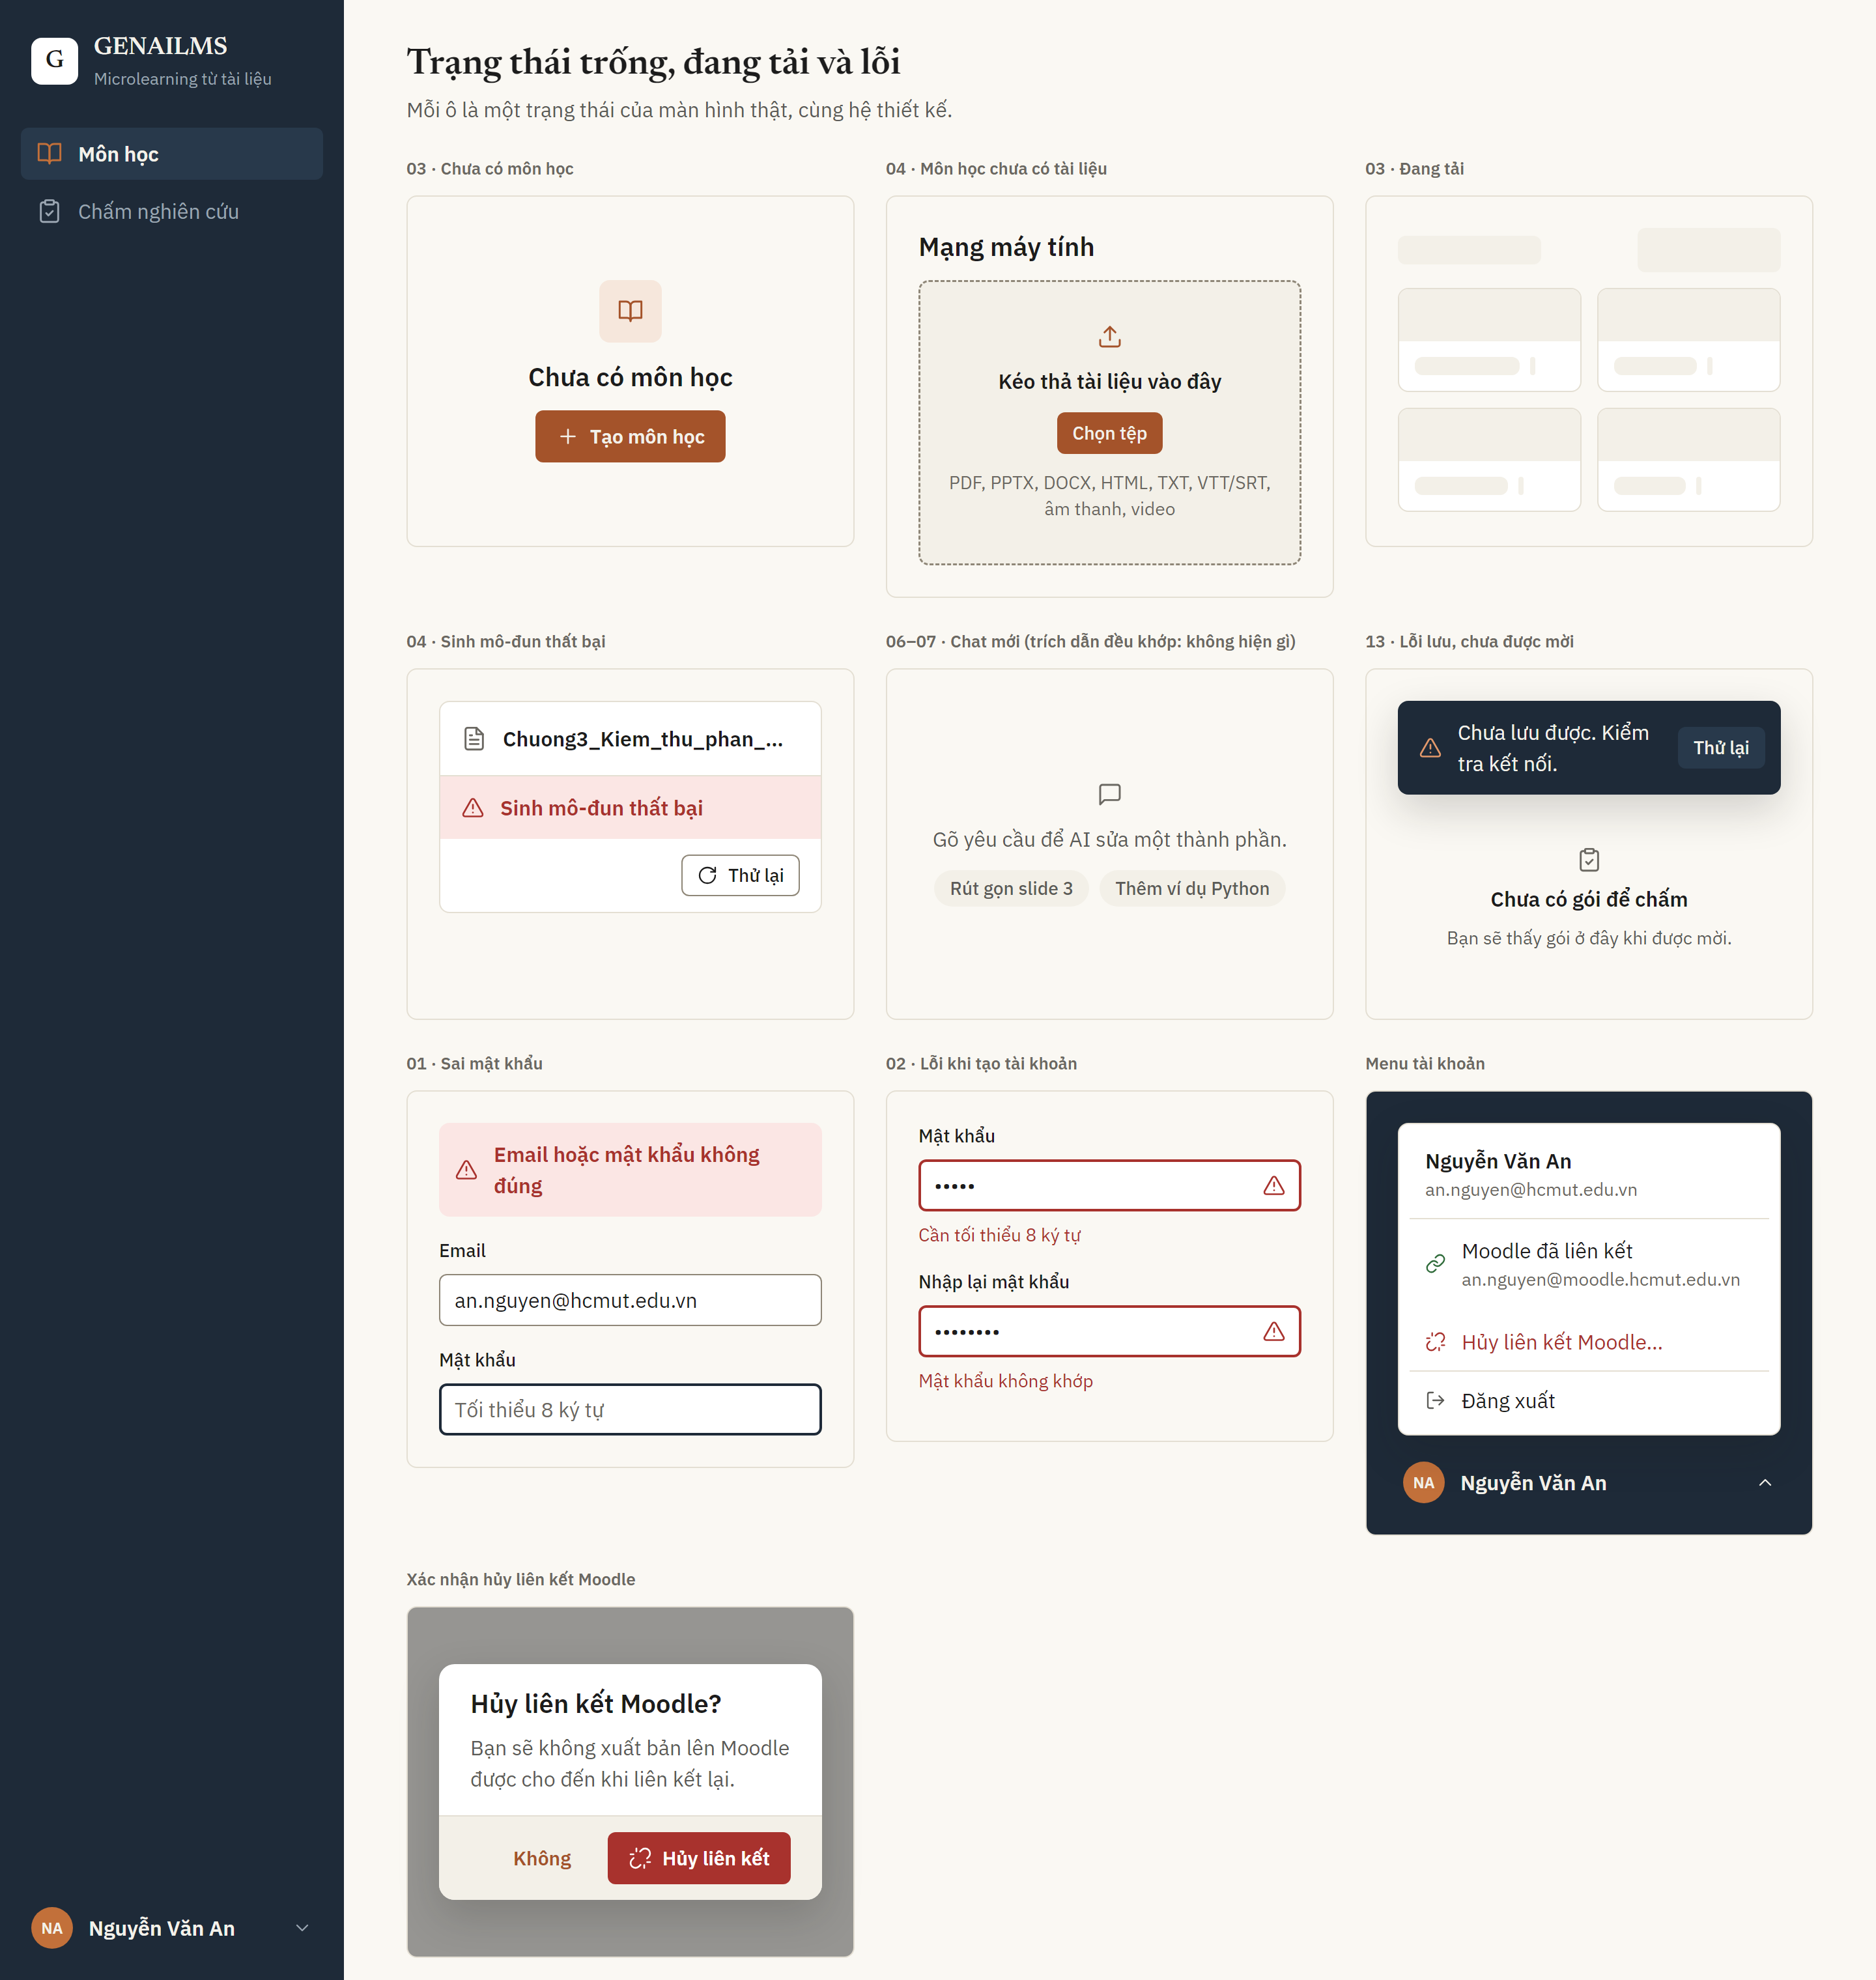
\includegraphics[width=.47\linewidth,height=.26\textheight,keepaspectratio,viewport={620 1480 1320 2000},clip]{graphics/ui/15-empty-loading-error-states.png}\hfill
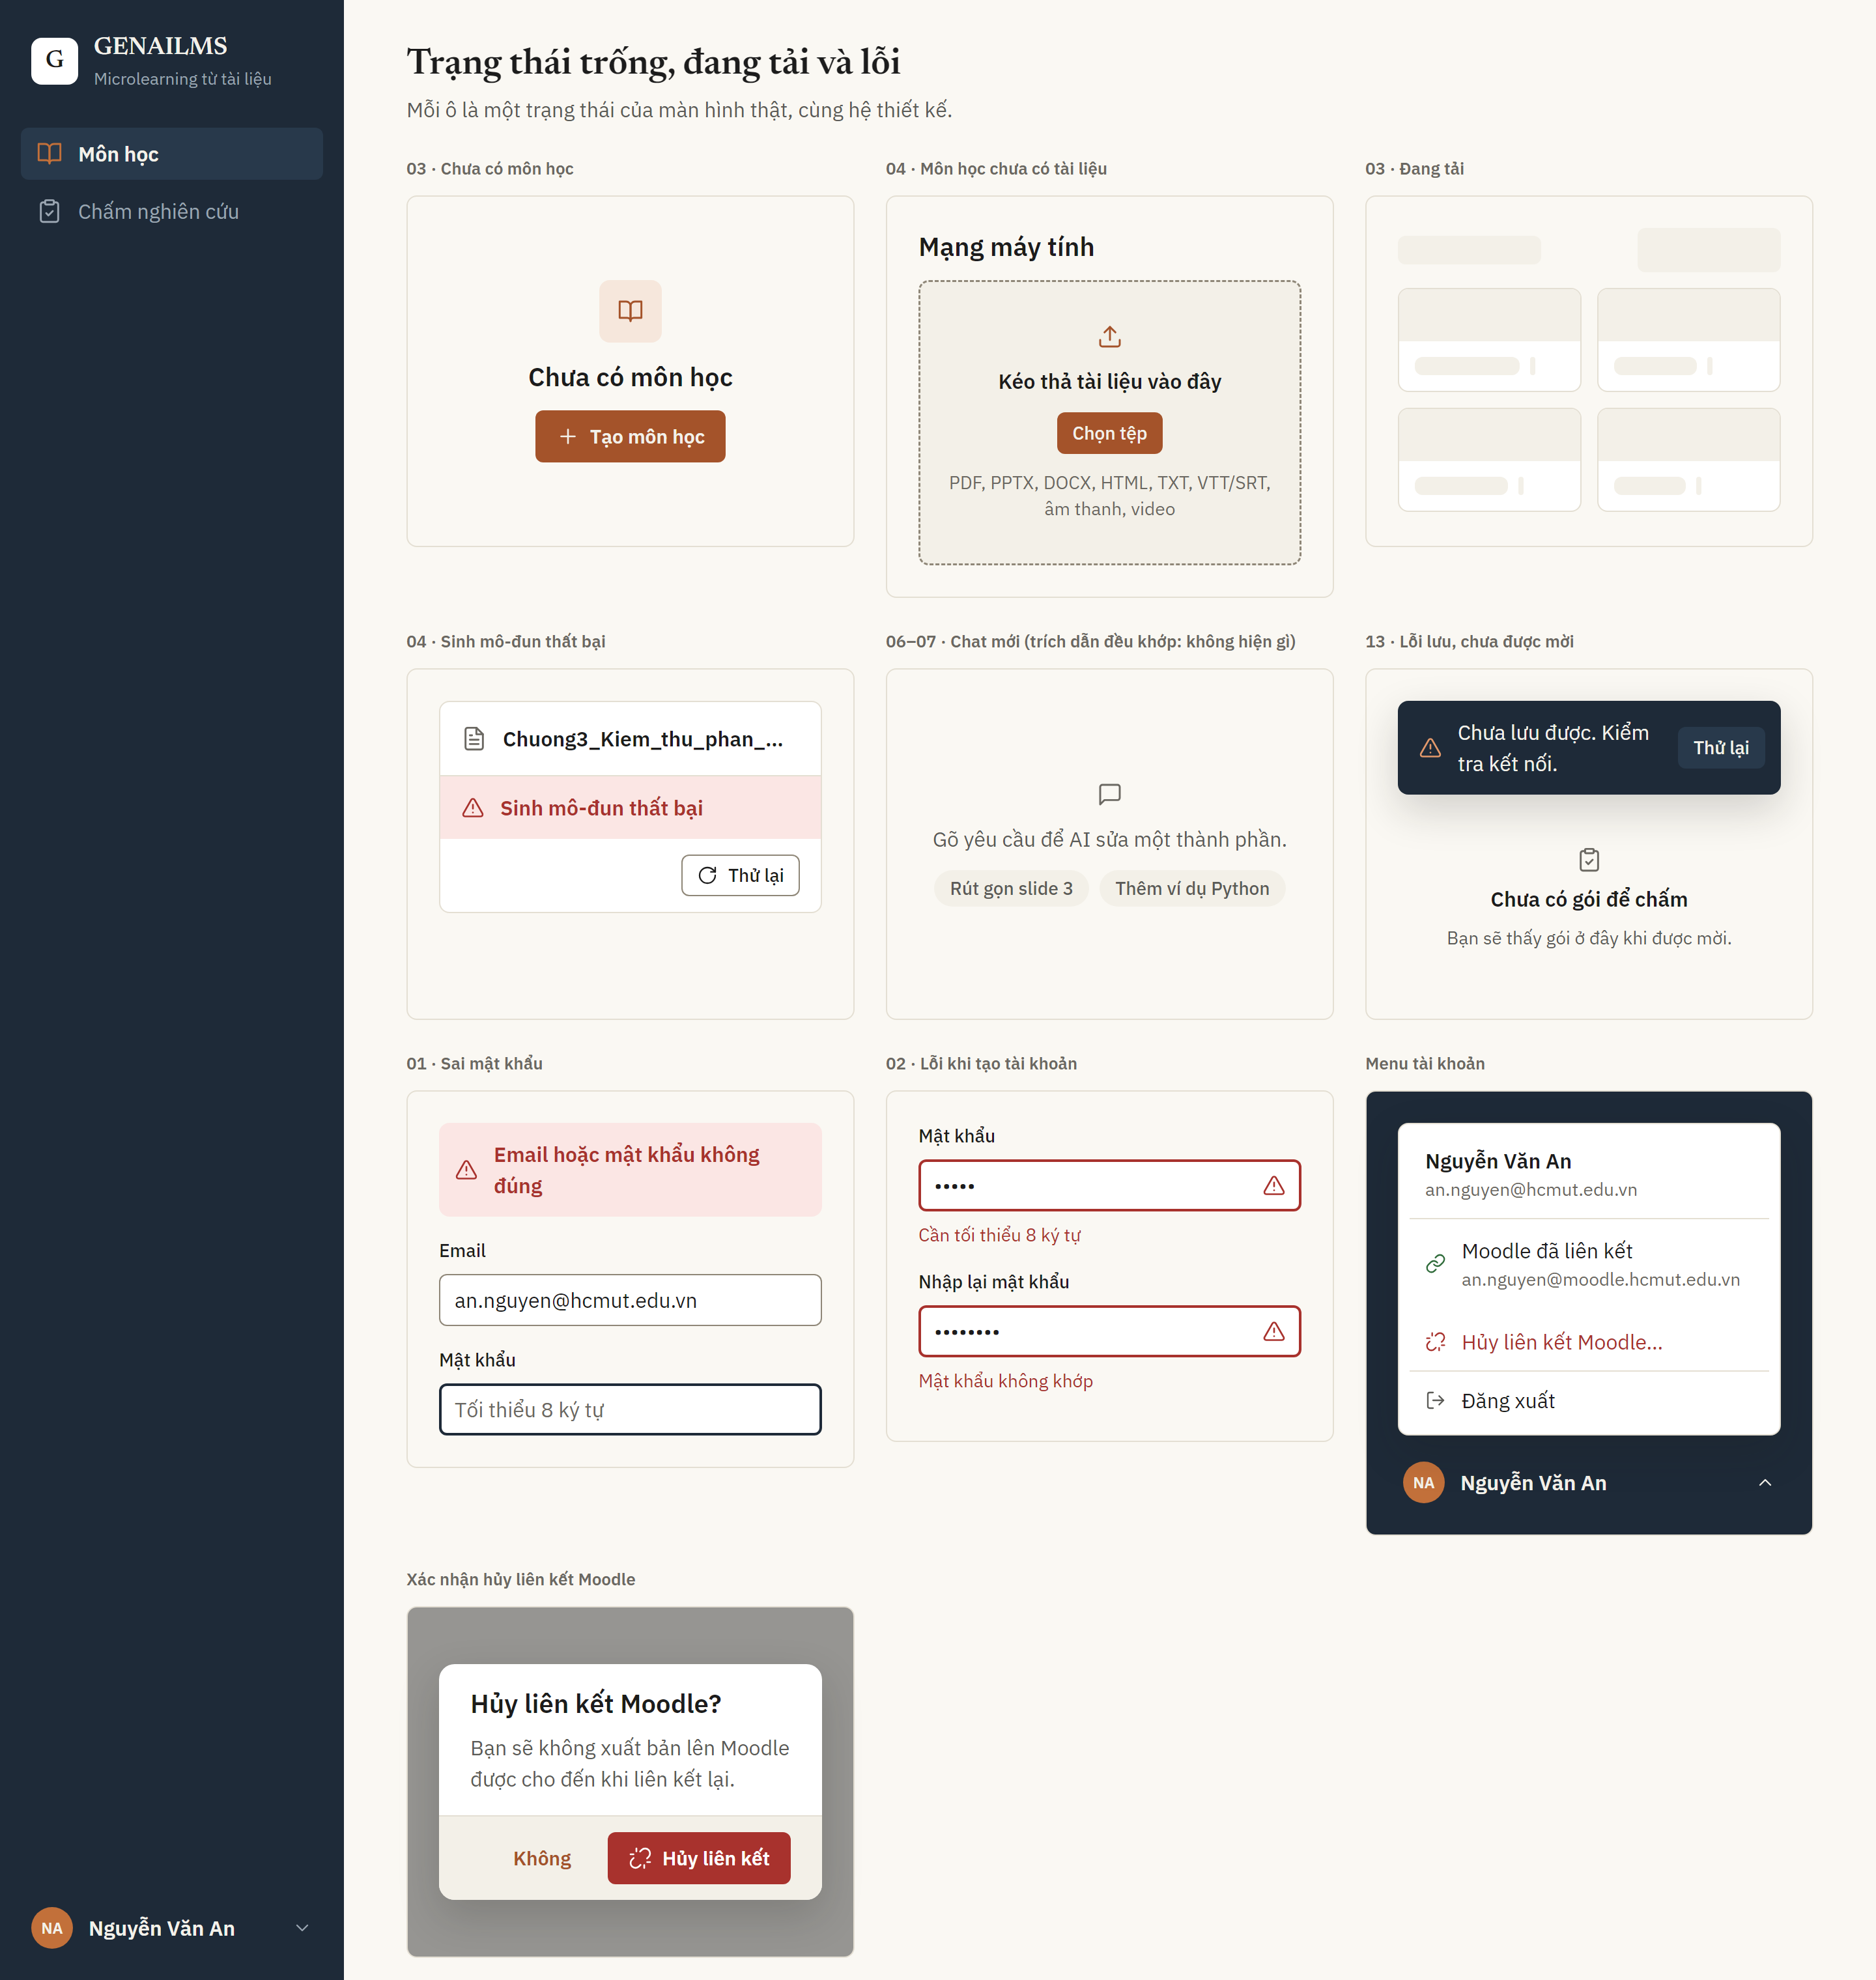
\includegraphics[width=.47\linewidth,height=.26\textheight,keepaspectratio,viewport={1360 1480 2050 2000},clip]{graphics/ui/15-empty-loading-error-states.png}\par\smallskip
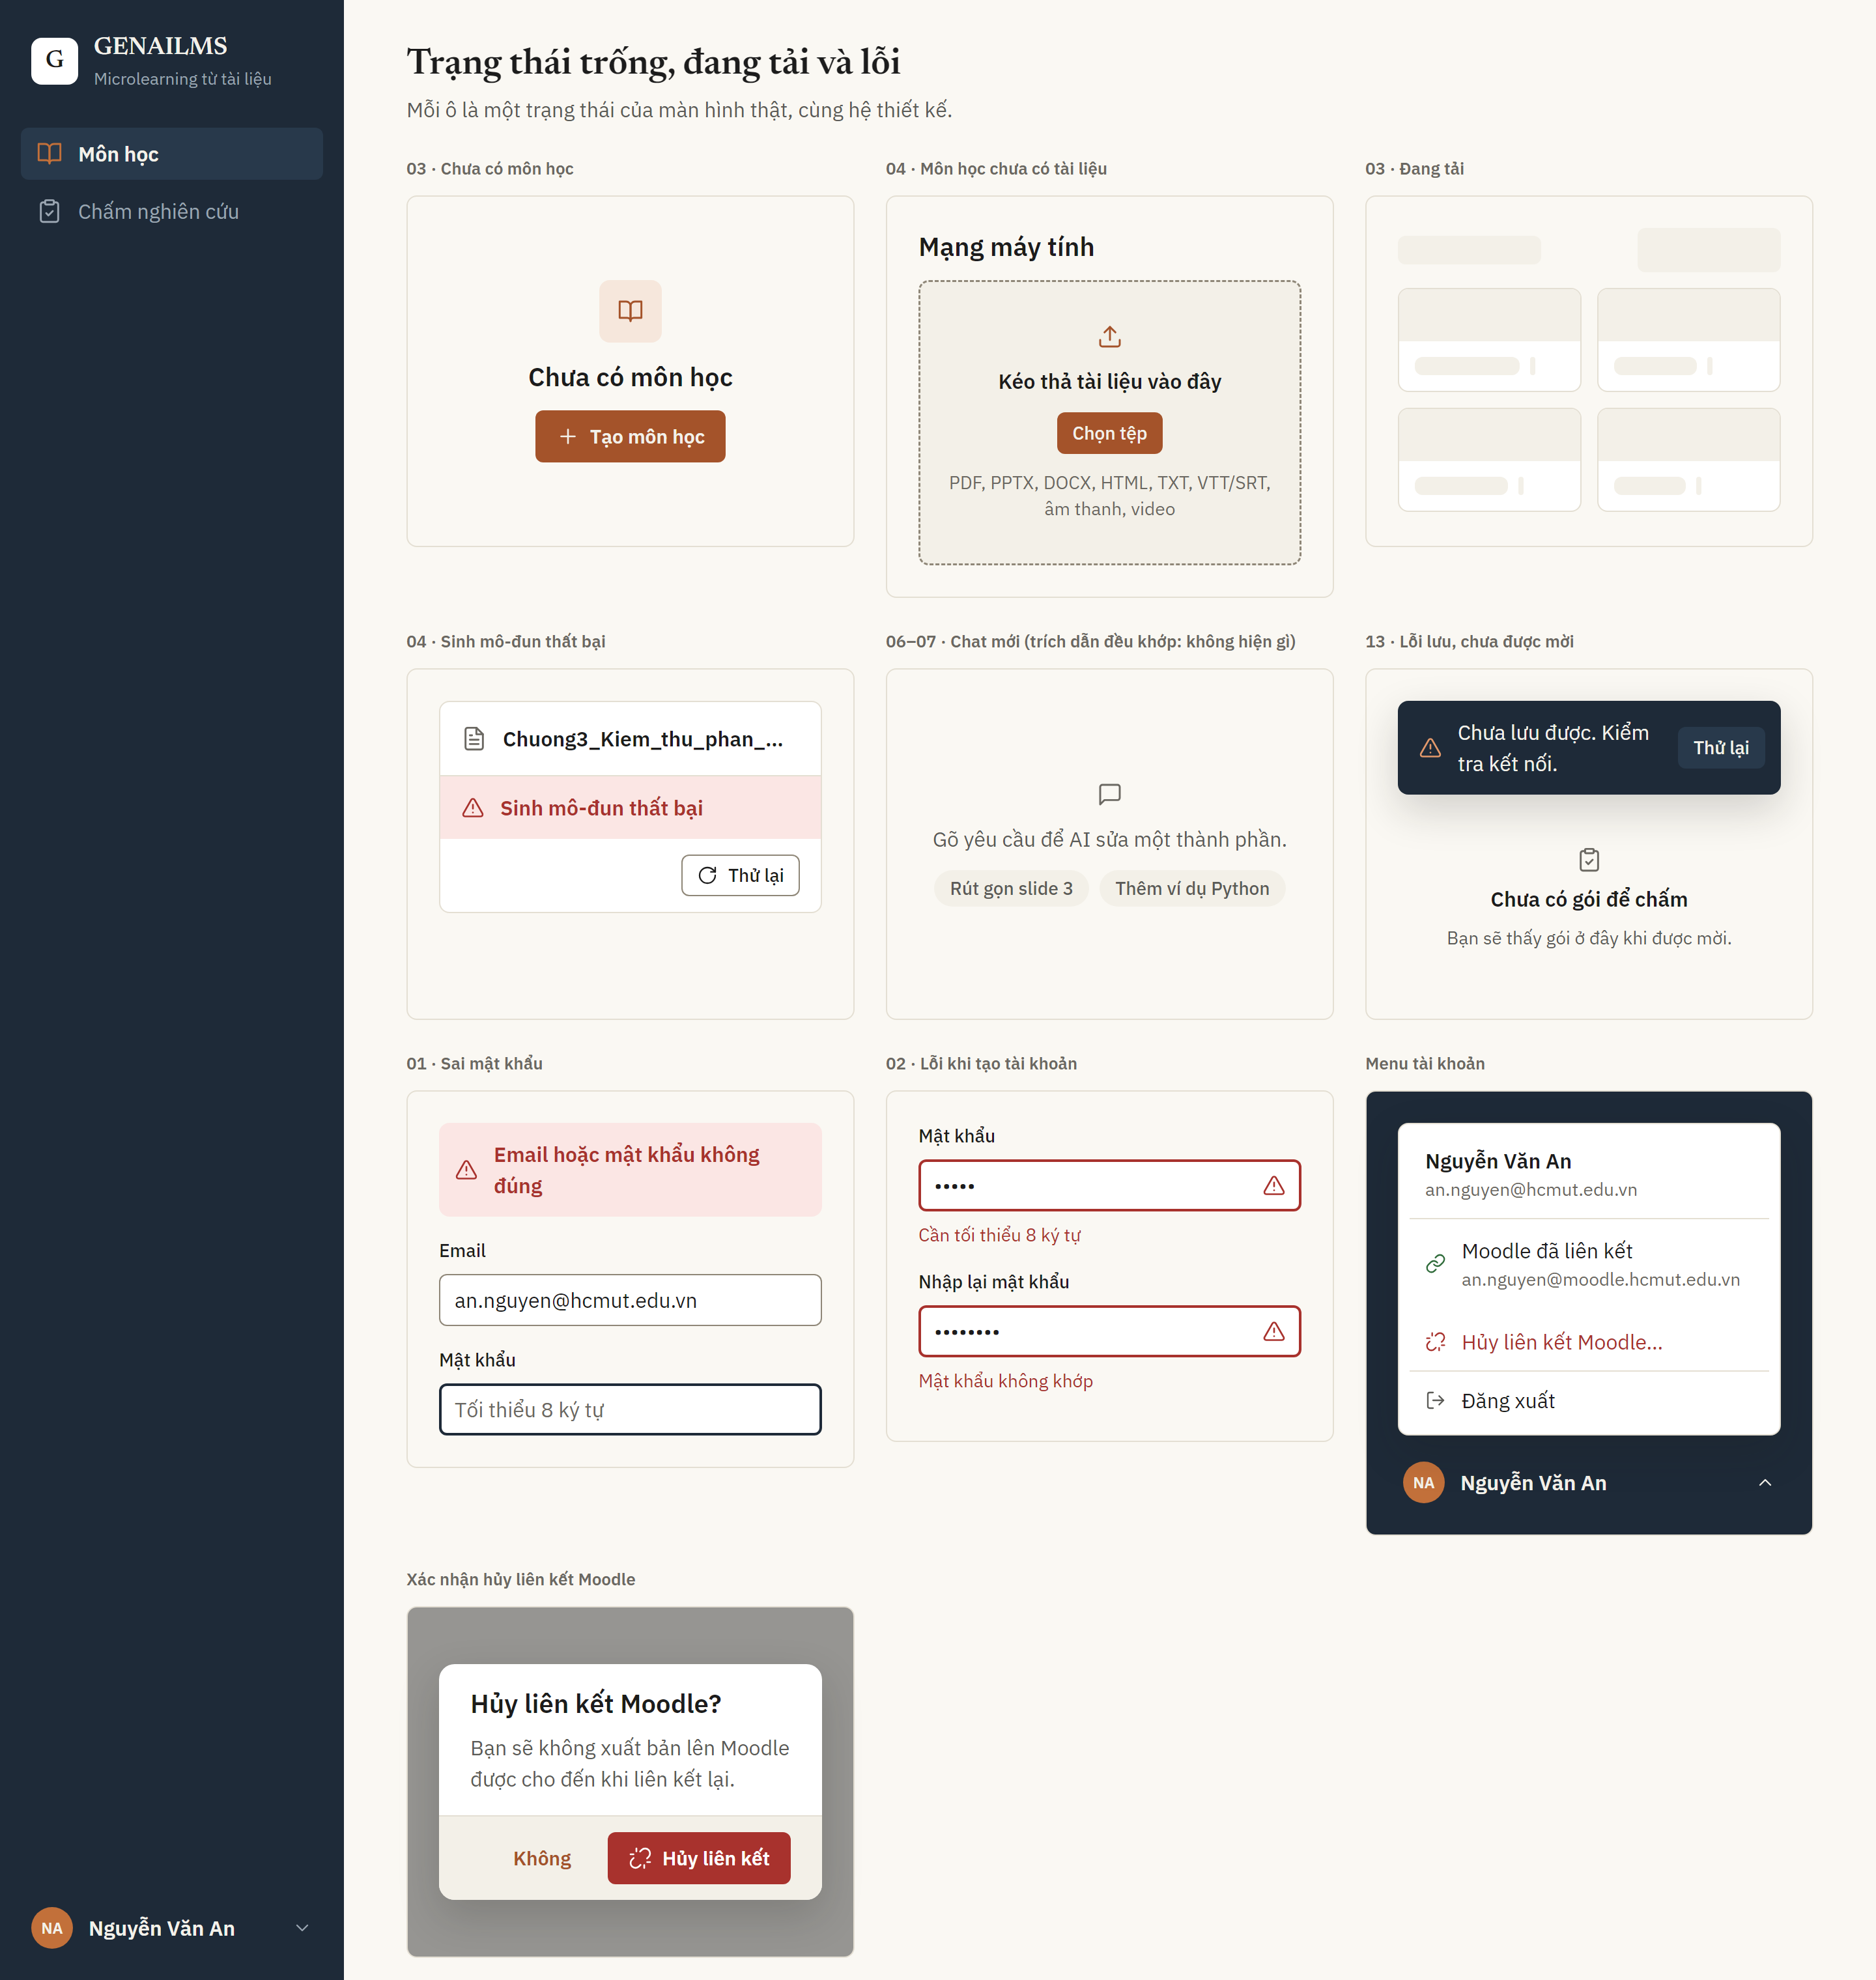
\includegraphics[width=.47\linewidth,height=.26\textheight,keepaspectratio,viewport={2100 1480 2800 2000},clip]{graphics/ui/15-empty-loading-error-states.png}\hfill
\caption{Failure recovery and empty conversation.}\label{fig:ui-screen-15-recovery}
\end{figure}

\needspace{.42\textheight}
Figure~\ref{fig:ui-screen-15-account} enlarges credential validation and account controls. ``Hủy liên kết Moodle'' means ``Unlink Moodle'' and ``Đăng xuất'' means ``Sign out''; unlinking requires confirmation because publication access changes.
\begin{figure}[H]\centering
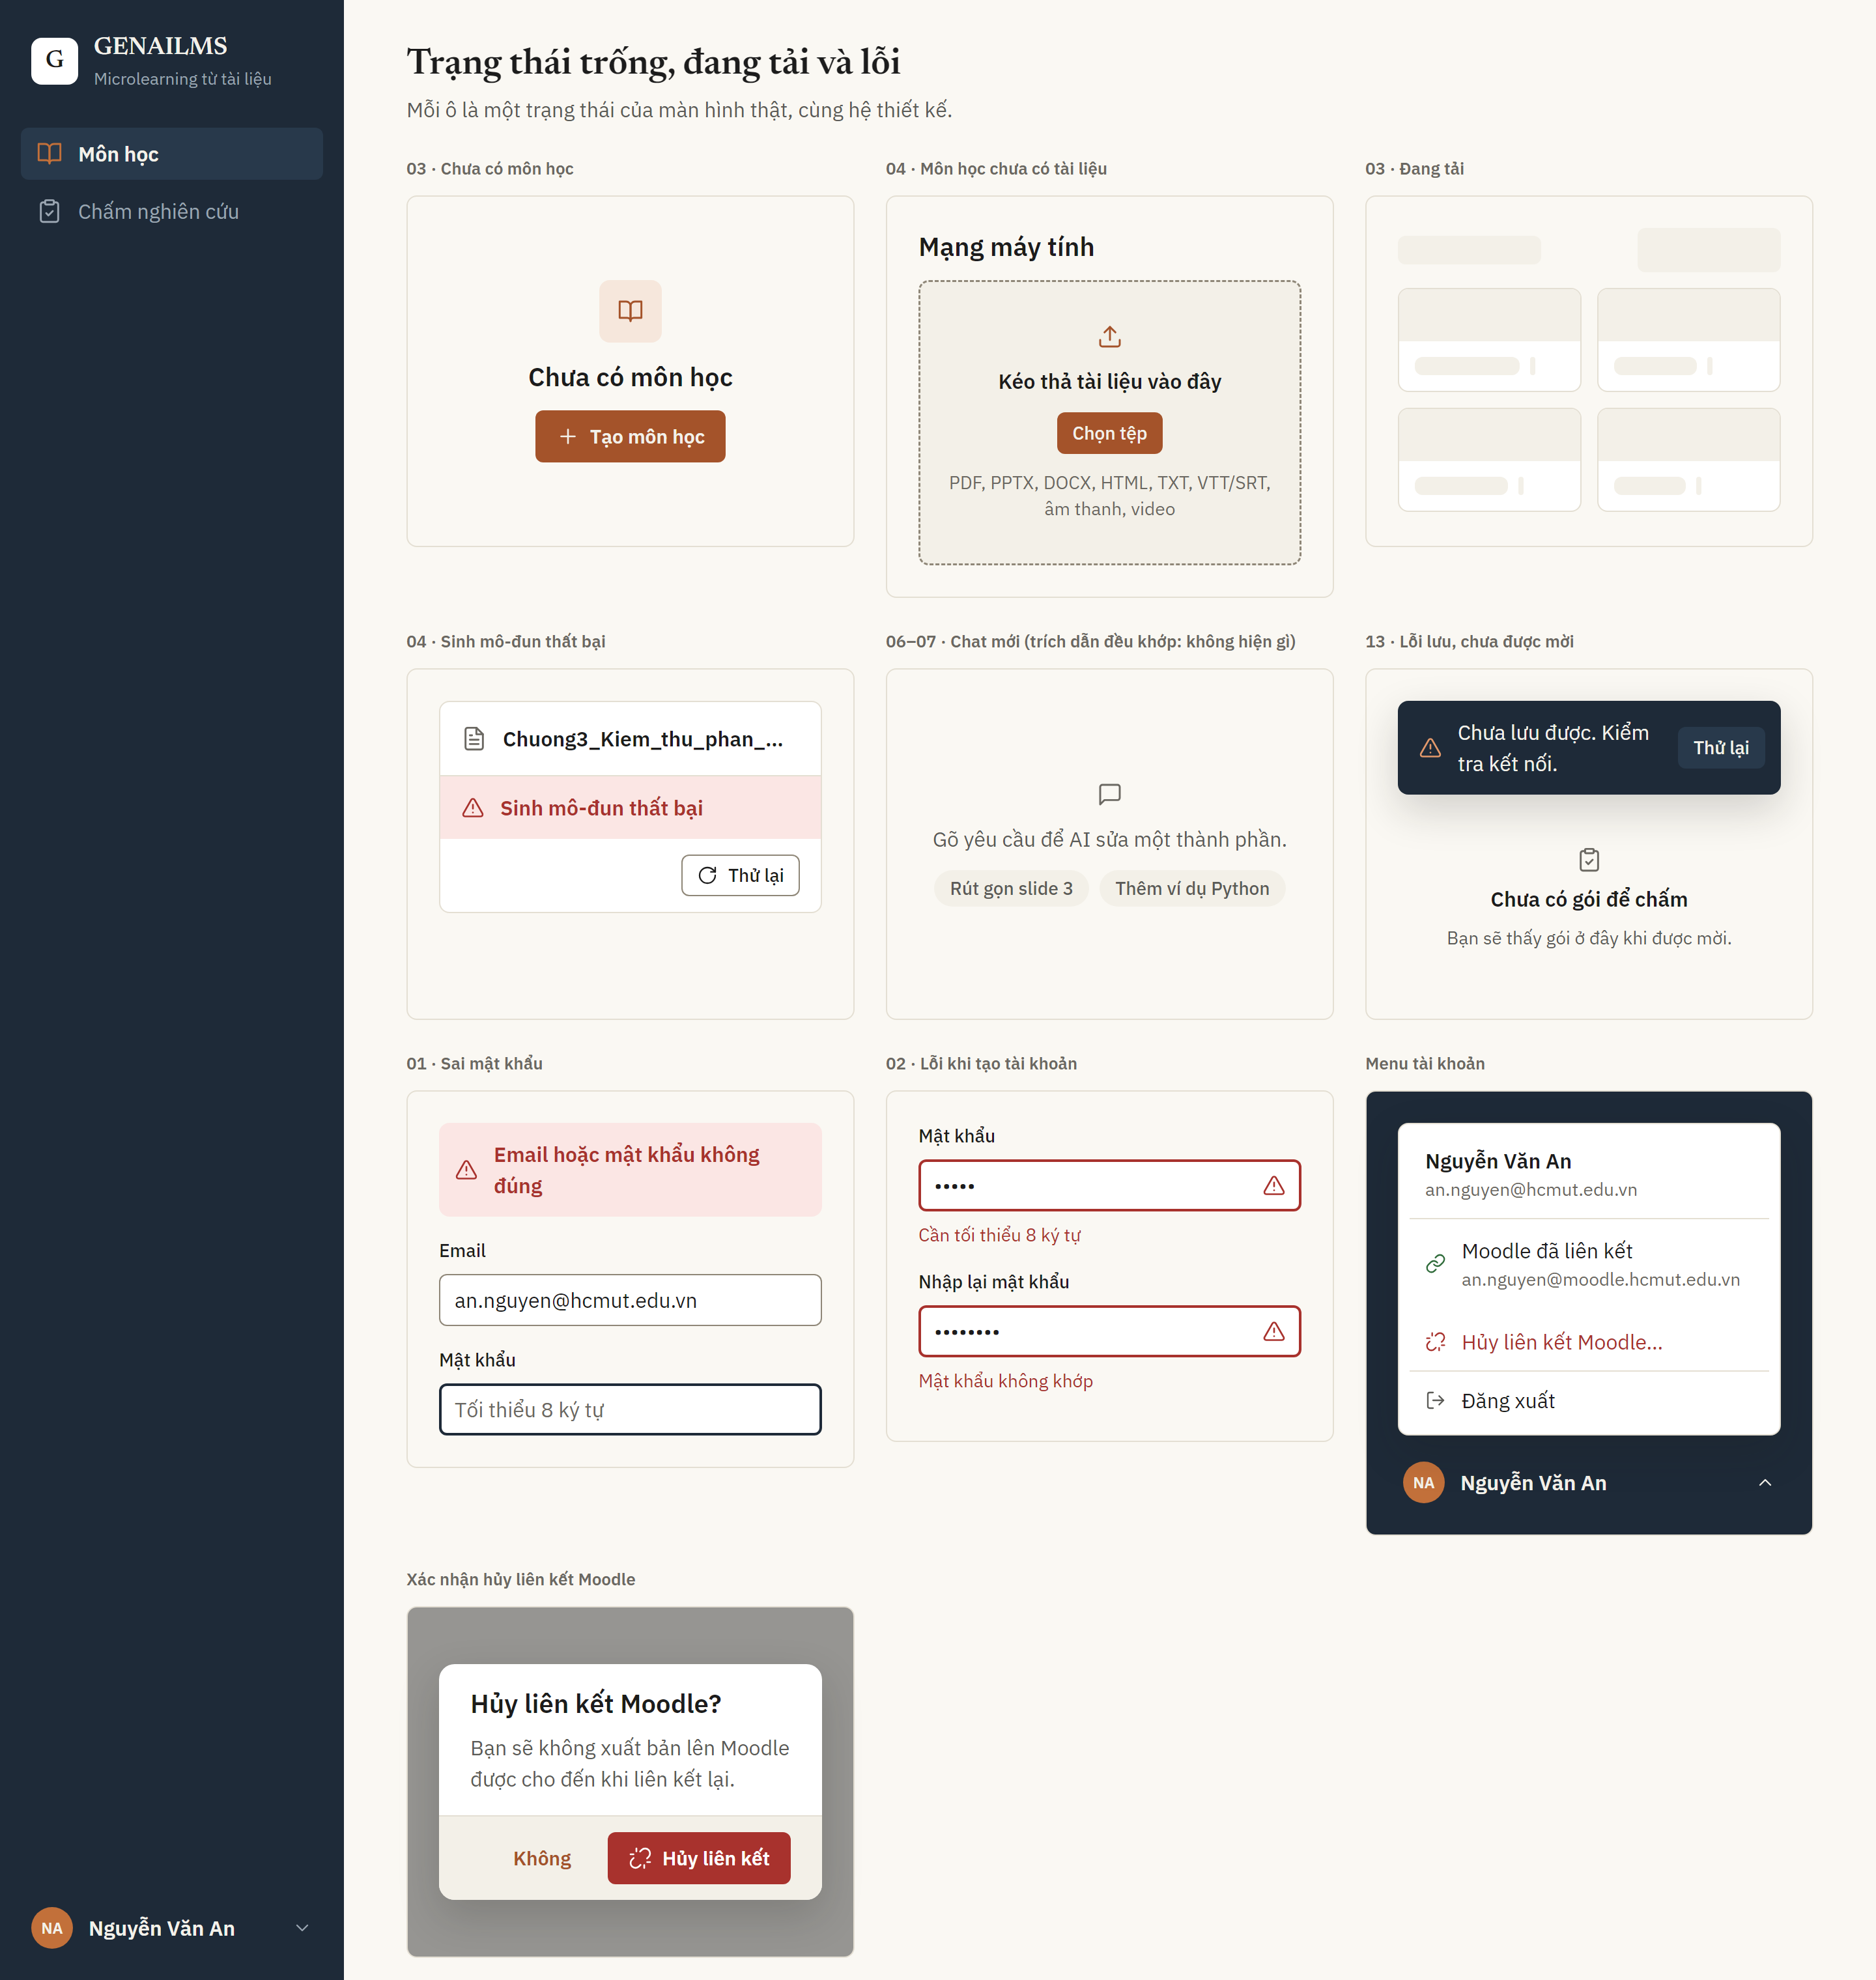
\includegraphics[width=.47\linewidth,height=.26\textheight,keepaspectratio,viewport={620 750 1320 1380},clip]{graphics/ui/15-empty-loading-error-states.png}\hfill
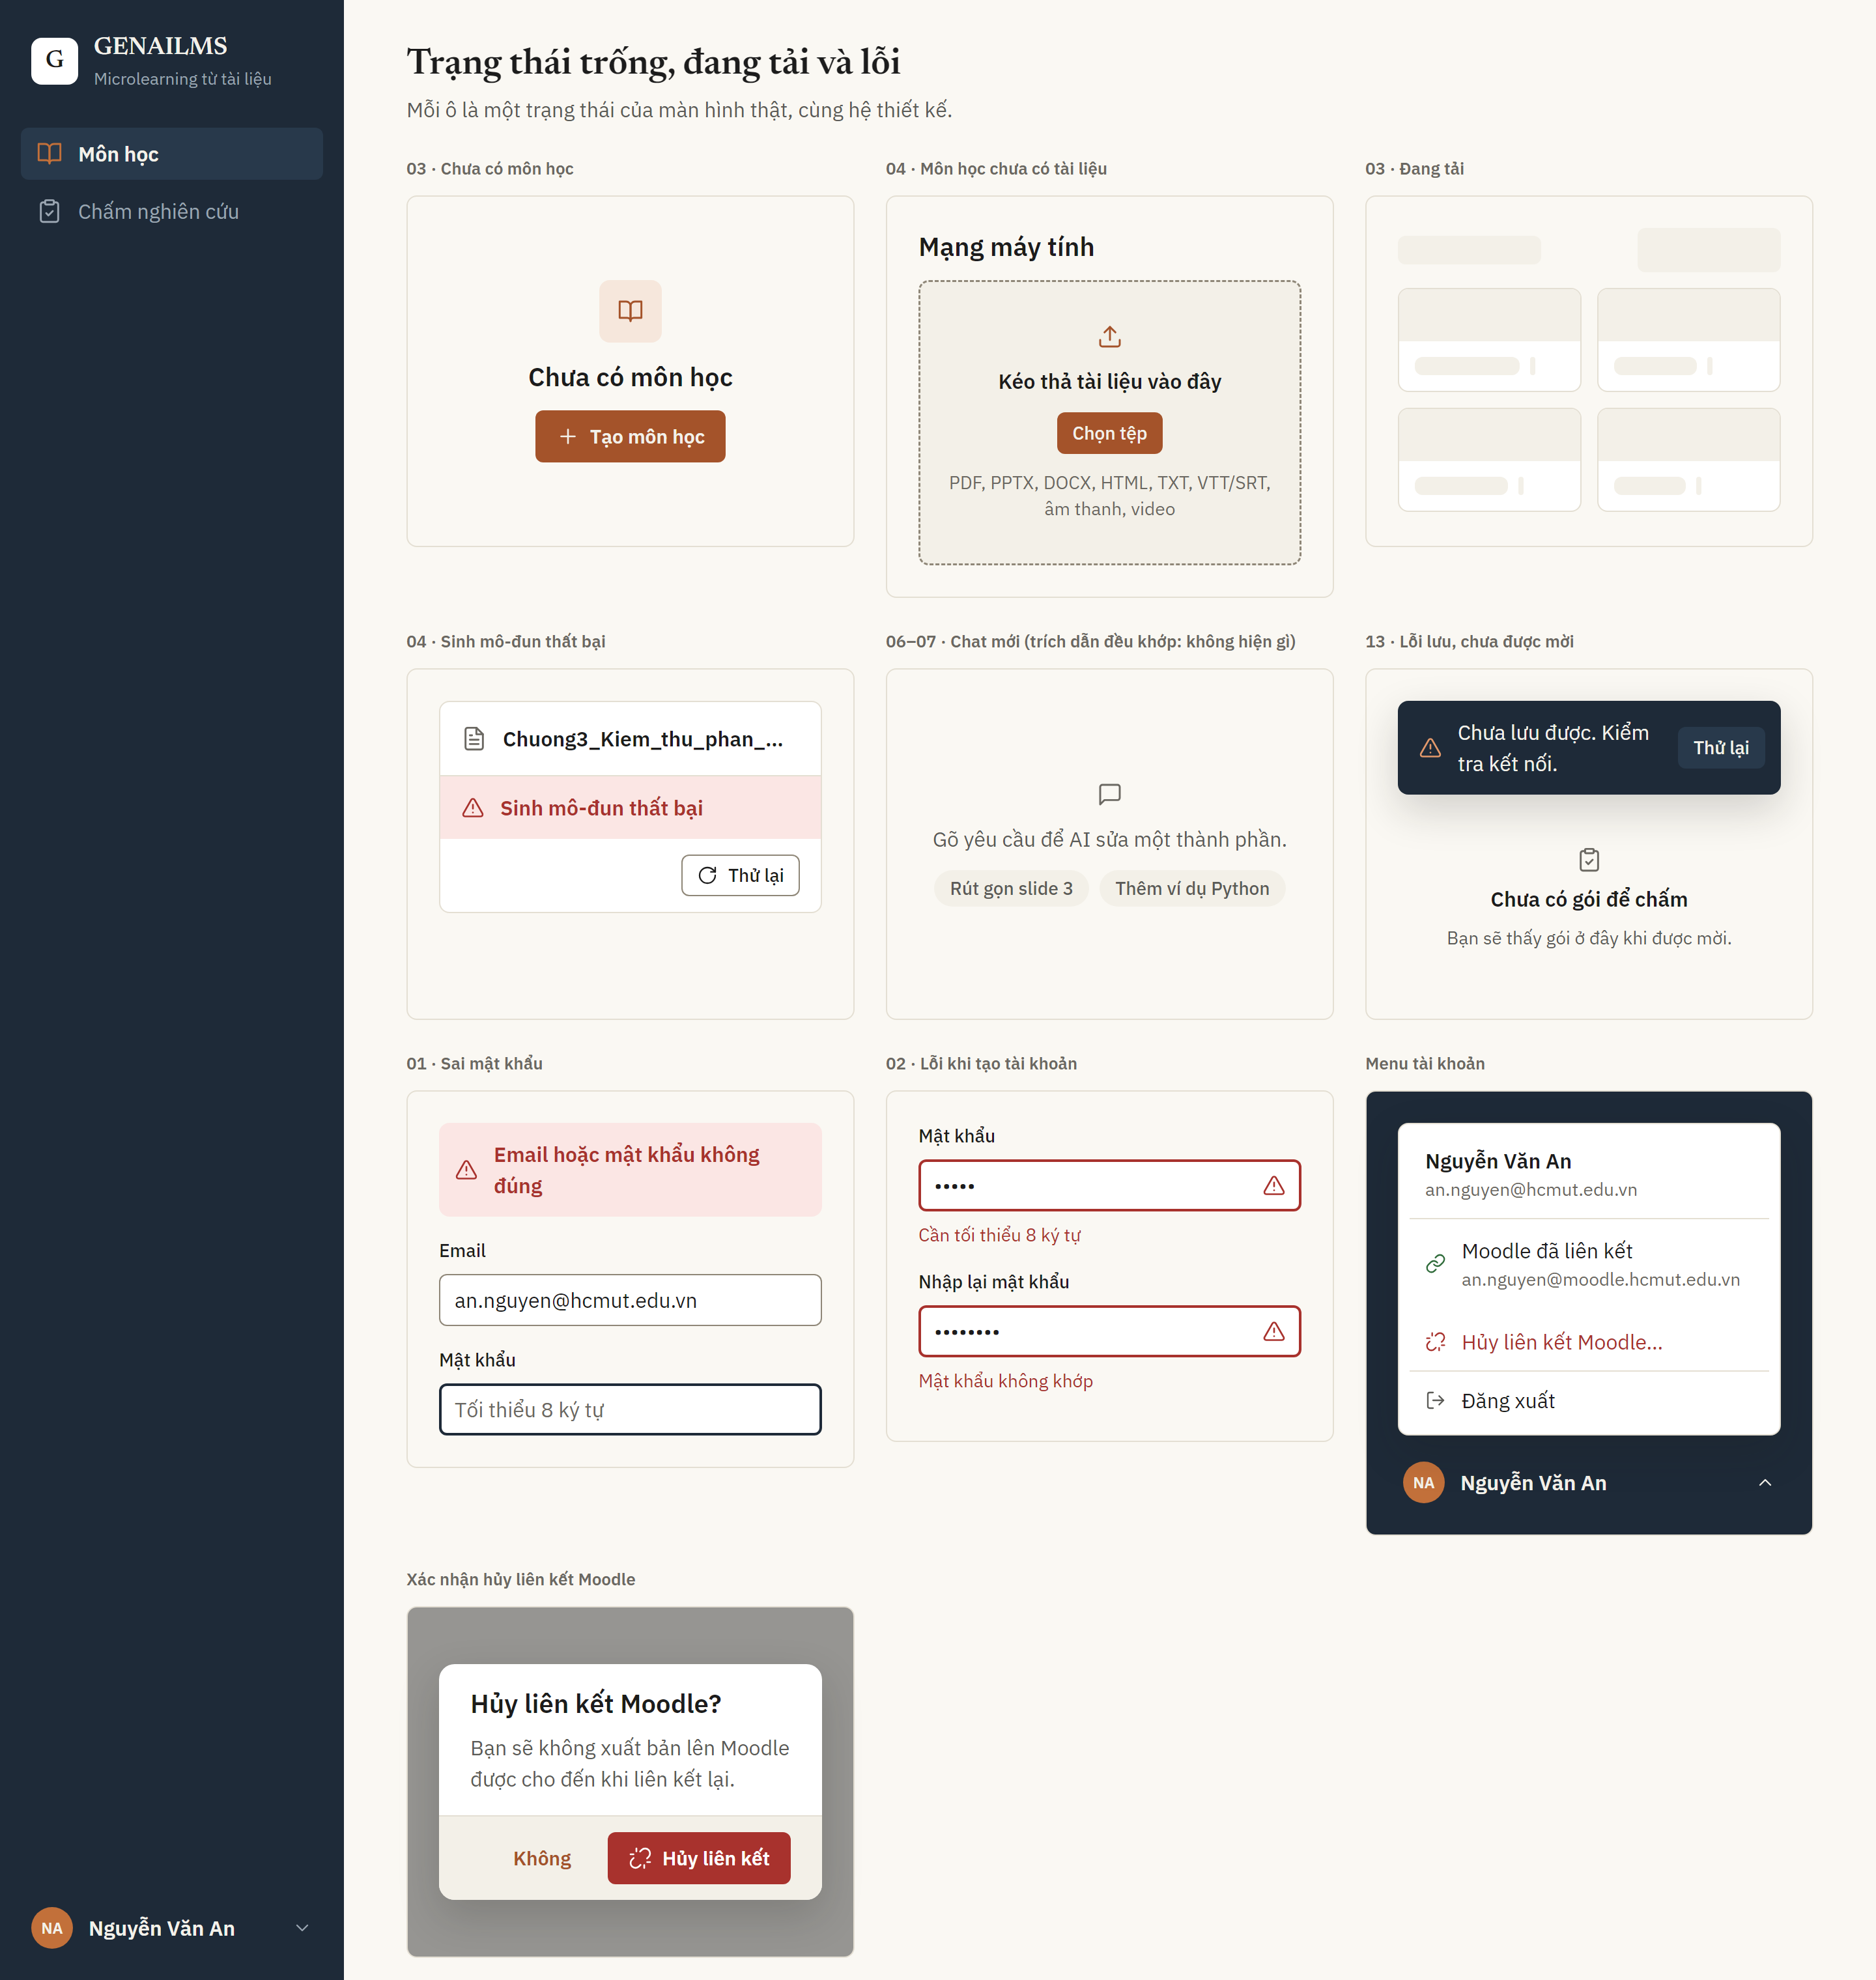
\includegraphics[width=.47\linewidth,height=.26\textheight,keepaspectratio,viewport={1360 790 2050 1380},clip]{graphics/ui/15-empty-loading-error-states.png}\par\smallskip
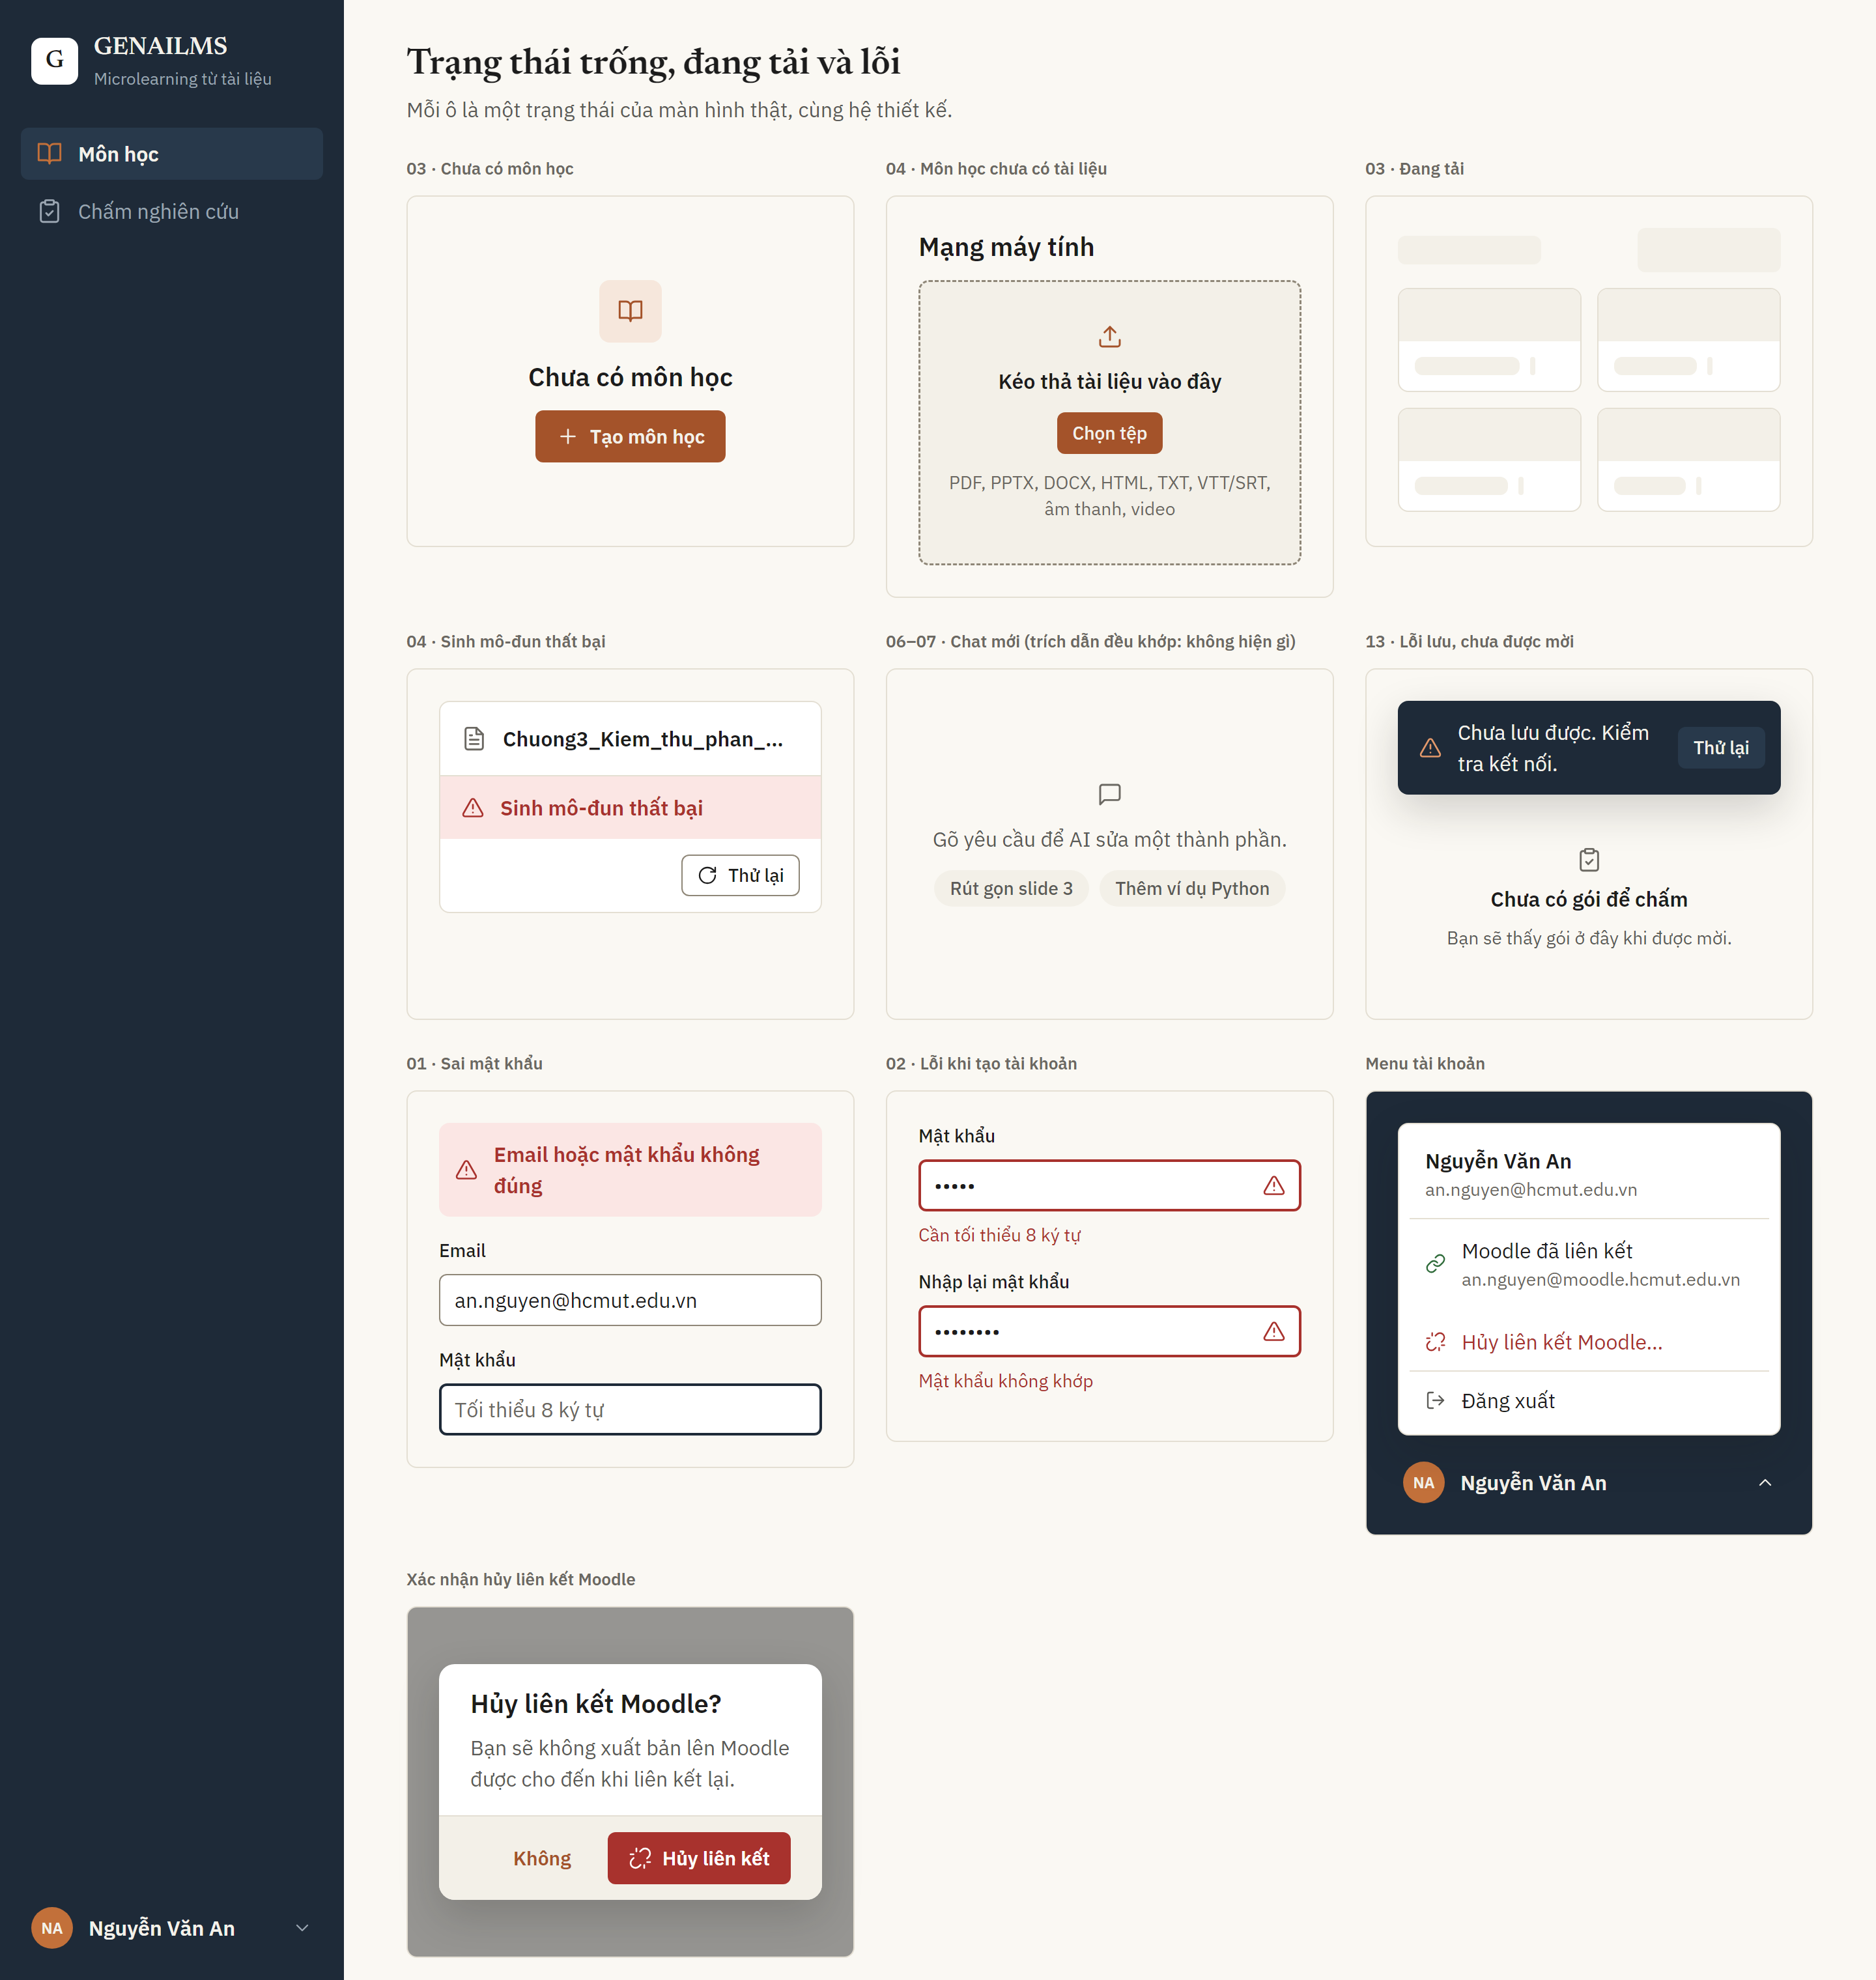
\includegraphics[width=.47\linewidth,height=.26\textheight,keepaspectratio,viewport={2100 640 2800 1380},clip]{graphics/ui/15-empty-loading-error-states.png}\hfill
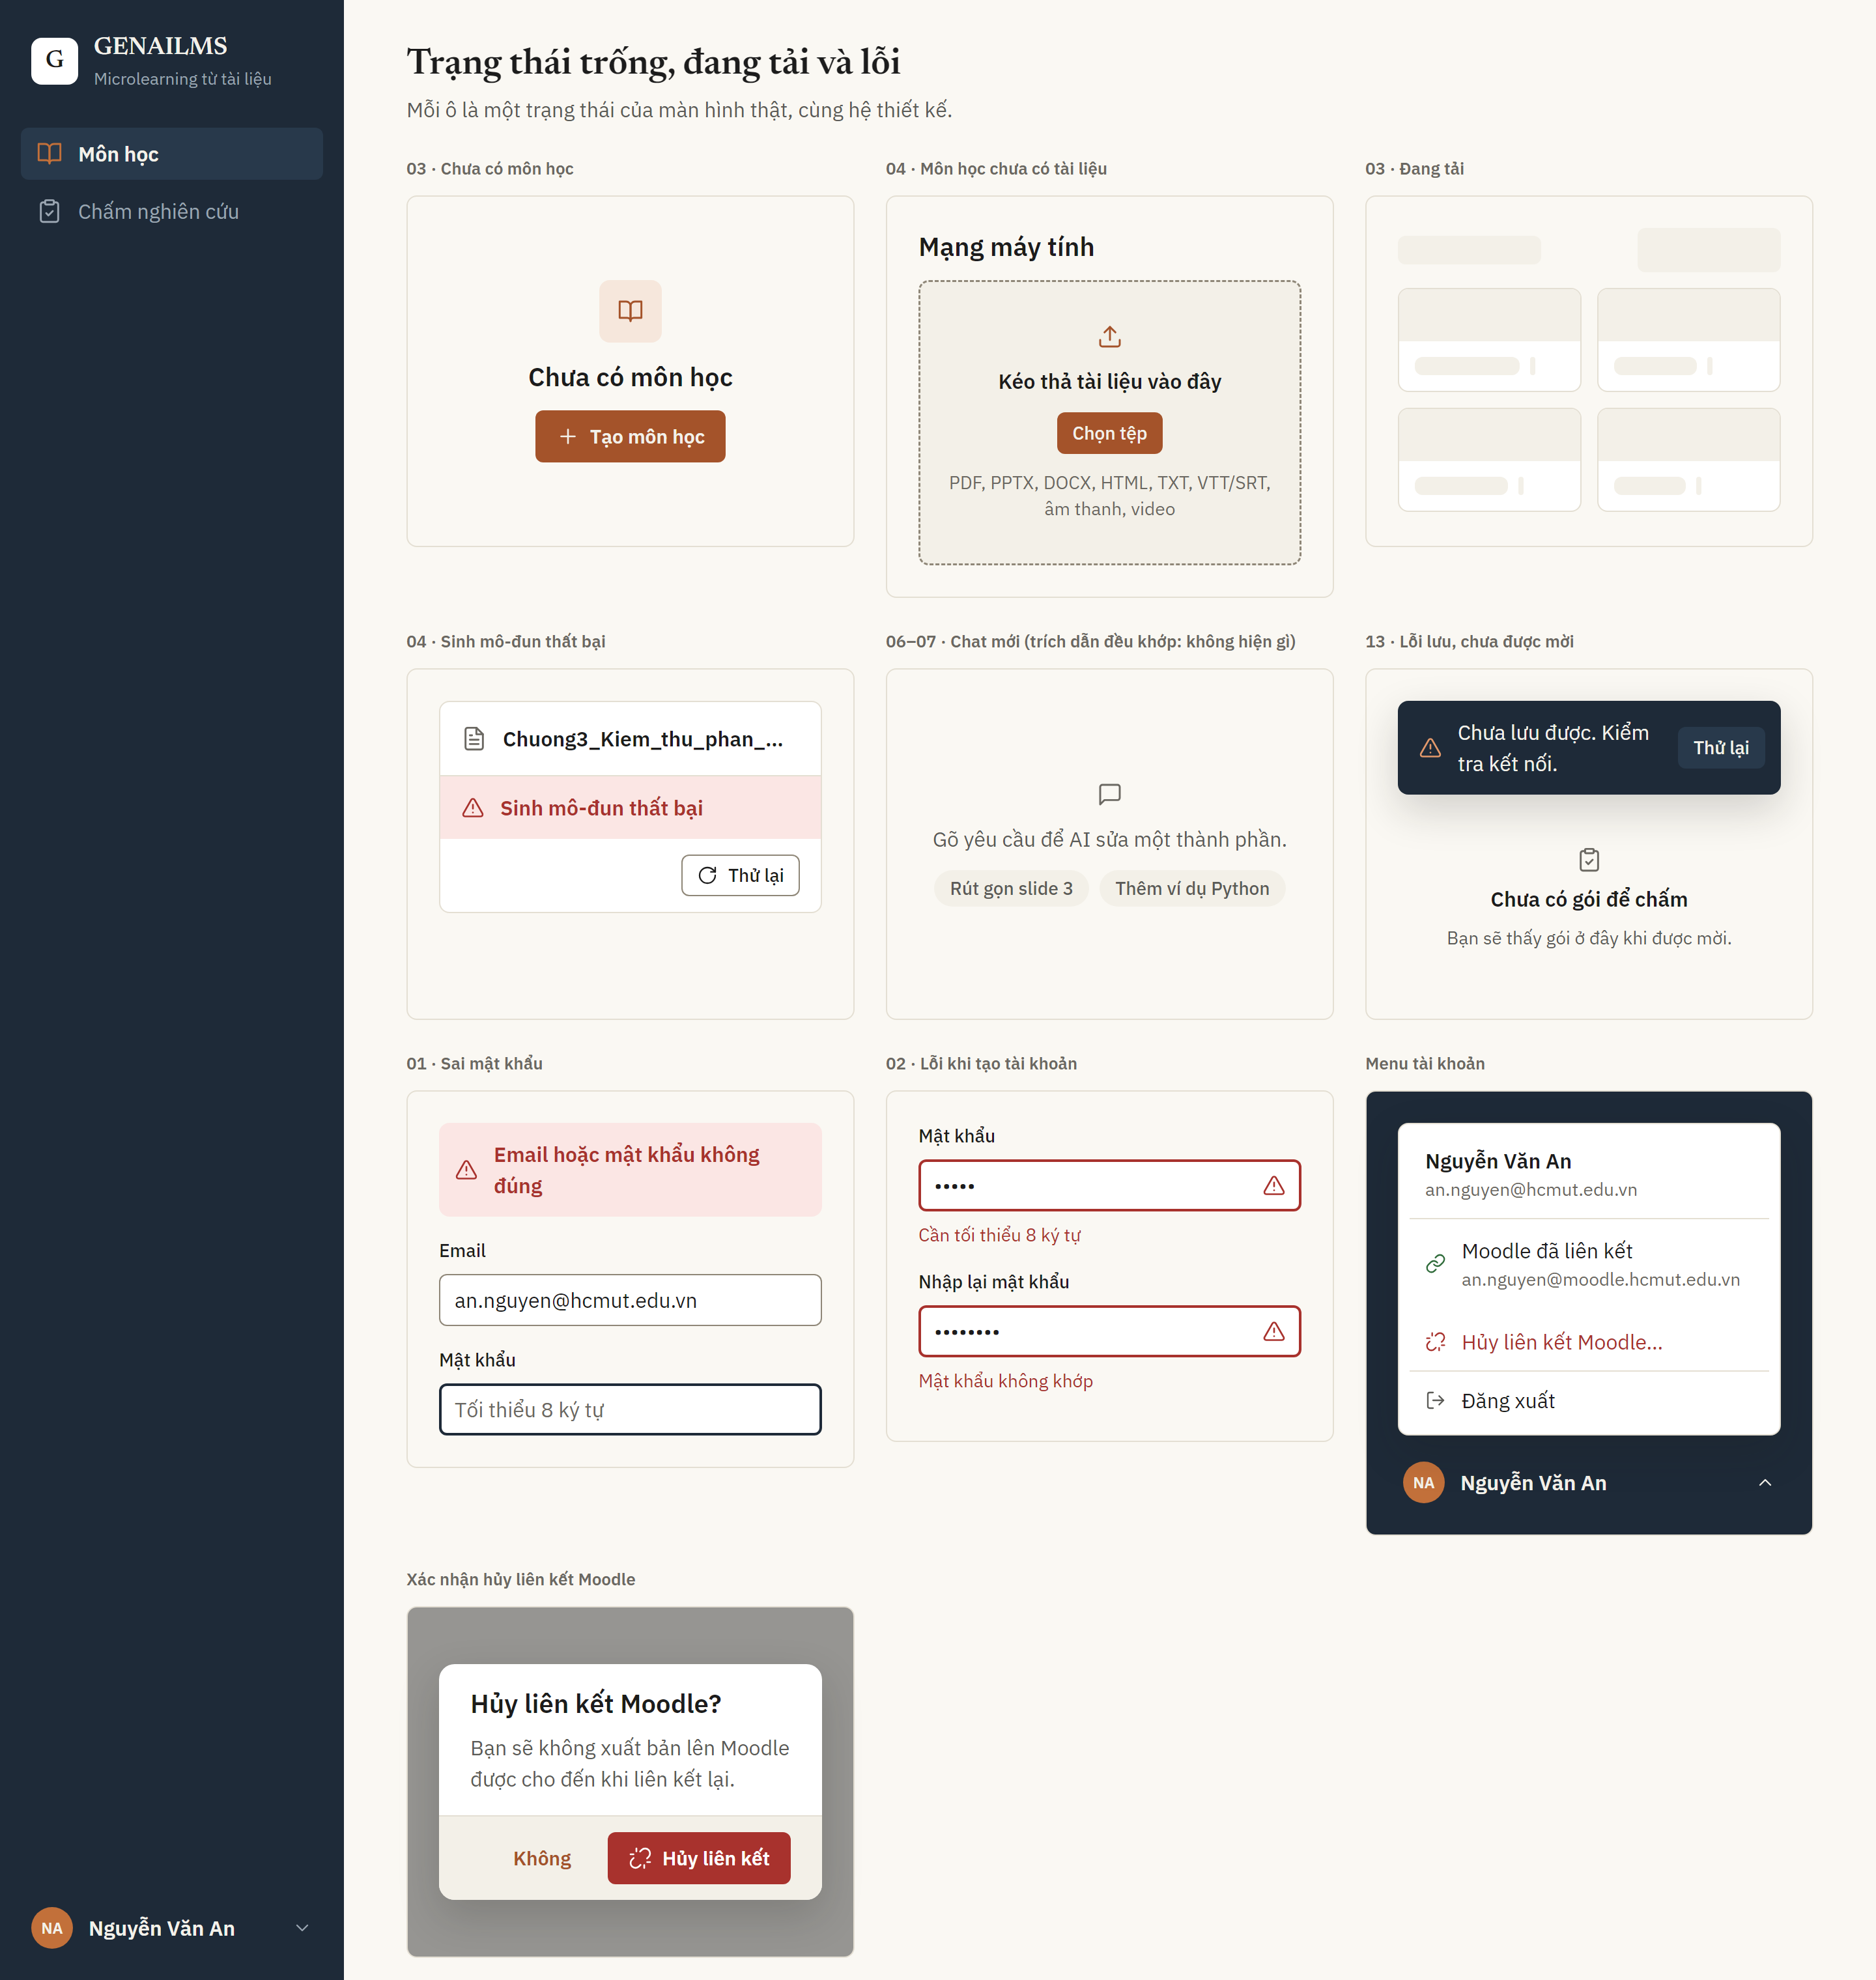
\includegraphics[width=.47\linewidth,height=.26\textheight,keepaspectratio,viewport={620 20 1320 580},clip]{graphics/ui/15-empty-loading-error-states.png}\par\smallskip
\caption{Validation, account menu and unlink confirmation.}\label{fig:ui-screen-15-account}
\end{figure}

\clearpage\section{Phase 2 evaluation design}\label{sec:evaluation}
\subsection{Research questions and experimental unit}
The evaluation measures both source support and pedagogical quality (Bloom alignment and question quality), so a strictly grounded but shallow configuration is not preferred. It asks whether source-conditioned generation improves factual support while maintaining completeness and question quality; whether inline citations support the associated claims; and which retrieval/reader choices provide suitable quality, latency and resource use.

The experimental unit is a topic/LO instance with a frozen source document and matched generation settings. RAG and LLM-only modules form pairs. Instructor-authored modules provide a human reference condition under common LO and structure requirements.
\subsection{Corpus and conditions}\label{sec:conditions}
The corpus contains Data Structures and Algorithms, Operating Systems, Programming Fundamentals and Web Programming. Development and held-out sets are split by document and checked for near duplicates. The inventory records language, format, permissions and code/formula content. Each pair uses a source hash and the same output language, model, guidance and self-check setting.

A pilot of five LO instances per subject yields 20 RAG/control pairs. The held-out target is 80 complete pairs (20 per subject), separate from the 20-pair calibration pilot. After the pilot, a document-clustered precision calculation will check whether 80 pairs can estimate the primary paired support-rate difference with a 95\% interval half-width at most 0.10; if not, recruitment extends in balanced blocks of four pairs to at most 120. The rule and final target are frozen before held-out generation; any shortfall is reported by subject. A stratified 12--20-packet double-rated subset will support human calibration.
\par
Table~\ref{tab:10-evaluation-1} presents experimental conditions and comparison purpose.
\begin{table}[H]\centering\small\caption{Experimental conditions and comparison purpose.}\label{tab:10-evaluation-1}
\begin{tabularx}{\linewidth}{|p{3.0cm}|Y|Y|}\hline
Condition & Input policy & Comparison purpose\\\hline
Human reference & Instructor-authored module at a common LO & Pedagogical reference and authoring effort\\\hline
LLM-only & Paired LO/settings; source block withheld & Source-withholding baseline\\\hline
RAG + LLM & Same settings plus retrieved evidence & Source-conditioned generation\\\hline
Self-check ablation & Matched subset with checks disabled & Effect and extra cost of checking\\\hline
Retrieval ablation & Dense, hybrid, reranked; fixed-$k$, then adaptive-$k$ & Separate ranking and context-budget effects\\\hline
Full-source subset & Bounded source text under common token budget & Retrieval versus document conditioning\\\hline
Stronger-model subset & Predeclared higher-tier paid model & Quality--cost tradeoff\\\hline
\end{tabularx}\end{table}

The paid generation model and local Qwen3 embedding revision are fixed for each comparison. Experiment mode disables cross-model fallback. The run record captures both selected alias and actual served model.
\subsection{Human rating and independent judges}
Invited raters receive anonymous packet snapshots, a stable per-rater shuffled order and common reference evidence. The rubric scores accuracy, completeness, consistency, source support, slide quality, quiz quality, Bloom fidelity and query alignment on a 1--5 scale. Each score has a reason; overall notes provide narrative feedback.

Practice packets calibrate interpretation before held-out rating. Packet text is checked for condition/model leakage. Human scores remain independent before adjudication. LLM judges use a model family distinct from the generator and a fixed prompt/reference set\citep{selfpreference}. Separate judge result packets record model, prompt and packet hash. Generator self-check is evaluated as a pipeline component, while human/independent judging supplies the comparison outcomes.
\subsection{Source support and citation metrics}
The grounding policy in Section~\ref{sec:grounding-policy} defines source-required material. Facts in lesson content, correct answers and their explanations are decomposed into atomic units with character spans, including source-required claims without markers. Explicitly labelled illustrative examples and model-generated distractors are excluded from the source-support denominator; they remain subject to consistency, execution where possible and pedagogical-quality checks. A human-audited sample calibrates extraction\citep{factscore}. Equation~\ref{eq:unsupported} defines the unsupported-claim rate:
\begin{equation}\label{eq:unsupported}
\mathrm{unsupported\_rate}=\frac{\text{unsupported atomic claims}}{\text{assessed atomic claims}}.
\end{equation}
Each packet records complete, partial or unknown reference coverage. A full rate requires an identified, nonempty reference set and a positive denominator; other packets retain their available judgments and are excluded from that aggregate.

Citation evaluation uses the passages directly attached to the claim\citep{alce}. Adjacent markers sharing a claim span can be assessed jointly, while Equation~\ref{eq:citation} defines entry-level citation accuracy:
\begin{equation}\label{eq:citation}
\mathrm{citation\_accuracy}=\frac{\text{supported assessed citation entries}}{\text{assessed citation entries}}.
\end{equation}
Span-level support is reported separately. Citation completeness measures the proportion of important source-required factual claims with a valid supporting citation. Marker validity, source-map resolution and span alignment provide diagnostic measures. Unresolved sources are retained as failures rather than replaced with another passage.
\subsection{Retrieval, extraction and usability}
Held-out English, Vietnamese and cross-language queries receive human labels allowing multiple relevant chunks. Retrieval measures Recall@$k$, mean reciprocal rank (MRR) and all-required-evidence coverage. Fixed-$k$ comparisons isolate ranking; adaptive selection is compared under the same ranking policy. Code/formula fidelity, missing text, reading order, locator accuracy and processing cost assess extraction.

Usability tasks cover uploading a source, generating a module, resolving a citation, editing, publishing and rating. Record completion, time, errors, recovery, keyboard access and participant feedback. Test empty, loading, validation, permission-loss and partial-publication states.
\subsection{Analysis and reproducibility}
Paired rubric comparisons use Wilcoxon signed-rank tests\citep{wilcoxon} with Holm correction\citep{holm}. Binary paired support outcomes use exact McNemar tests\citep{mcnemar}. Spearman correlation\citep{spearman} and quadratic weighted kappa\citep{weightedkappa} assess judge agreement. Report sample counts, distributions, effect sizes and confidence intervals. Bootstrap\citep{bootstrap} at document/pair level to account for correlated claims; unpaired human reference comparisons use separate descriptive or unpaired analysis.

The experiment manifest records source hashes, reader/chunker settings, embedding/reranker revisions, prompt/schema versions, selected/served models, language, LO, retrieval budget, self-check/fallback policy, pair/packet hashes, hardware and concurrency. Preserve raw AI output and reference snapshots before instructor editing. Measure all attempts, tokens, wall-clock time, peak memory and charges, separating provider usage from local hosting cost.

\clearpage\section{Design synthesis and Phase 2 plan}\label{sec:plan}
\subsection{Design outcomes}
The design connects an instructor-owned course workspace, asynchronous document processing, local multilingual retrieval, seven-part generation, physical inline citations, preservation of the AI original, Moodle publication and blinded evaluation. Its central invariants are ownership isolation, stable source identity, consistent question/explanation edits and separation of teaching content from evaluation snapshots.

Exploratory comparisons guide Qwen3 embedding, multilingual Jina reranking, bounded context and lightweight PDF extraction. Phase 2 will integrate the specified services and test these choices on held-out computing documents under fixed model conditions.
\par
Table~\ref{tab:11-plan-1} presents designed subsystems and their validation targets.
\begin{table}[H]\centering\small\caption{Designed subsystems and their validation targets.}\label{tab:11-plan-1}
\begin{tabularx}{\linewidth}{|p{3.0cm}|Y|Y|}\hline
Subsystem & Design specification & Phase 2 validation\\\hline
Authoring & Owned courses, asynchronous jobs, seven-part modules and editing & Complete instructor task flow and recovery\\\hline
Retrieval & Qwen3, BM25/RRF, Jina INT8, bounded adaptive context & Multilingual evidence coverage and resource use\\\hline
Citations and originals & Physical source map, inline spans and immutable AI snapshot & Claim/source alignment and edit consistency\\\hline
Moodle boundary & Confirmed actor, course capabilities and activity mapping & Permission loss and partial-write recovery\\\hline
Interface & Fifteen screens with role-specific navigation and source review & Accessibility and task-based usability\\\hline
Evaluation & Paired conditions, blinded snapshots and independent judging & Rubric agreement, citation support and cost\\\hline
\end{tabularx}\end{table}
\subsection{Dependency-driven schedule}
The twelve-week planning baseline runs from 26 October 2026 to 17 January 2027. The target defense/demo milestone is 18 January 2027; the faculty schedule determines the final appointment. Table~\ref{tab:schedule} and Figure~\ref{fig:gantt} align work windows with their exit criteria.
\begin{longtable}{|p{2.0cm}|p{6.9cm}|p{5.0cm}|}\caption{Phase 2 work packages and exit criteria.}\label{tab:schedule}\\\hline
Window & Work package & Exit criterion\\\hline\endfirsthead
\hline Window & Work package & Exit criterion\\\hline\endhead
26 Oct--8 Nov & Develop ownership, ingestion, physical citation mapping and AI-original preservation; prepare corpus and raters & Consistent source scope and frozen experiment protocol\\\hline
2--15 Nov & Develop retrieval/gateway orchestration; label gold queries and prepare human packets & Calibrated retrieval labels, rubric and reference packets\\\hline
9--22 Nov & Pilot paid-model paired generation and measure failure/cost & Refined workload and fixed held-out settings\\\hline
16 Nov--6 Dec & Generate held-out pairs and bounded retrieval/self-check ablations & Complete raw packets and attempt records\\\hline
23 Nov--13 Dec & Conduct blinded rating, independent judging and claim audits & Agreement sample and documented adjudication\\\hline
7--20 Dec & Analyze quality, source support, retrieval and cost & Effect sizes, uncertainty and subject-level error analysis\\\hline
14 Dec--3 Jan & Develop interface and publication recovery; conduct usability/security scenarios & Task observations and safe recovery evidence\\\hline
28 Dec--17 Jan & Prepare demonstration, final report and evaluation package & Reproducible experiment artifacts and final analysis\\\hline
\end{longtable}
\diagram{phase2-gantt}{Phase 2 planning baseline, with a target defense milestone after week twelve.}{gantt}
\subsection{Engineering priorities}
Physical source identity and original preservation precede formal data collection. Model, prompt and corpus versions remain fixed within a comparison. Publication recovery records external activity IDs and per-step outcomes. Source-quality checks identify missing or malformed pages. User feedback and security scenarios guide the final interface and deployment configuration.

\subsection{Risks and mitigations}
Table~\ref{tab:risks} records the main limitations that can affect delivery or validity. Each trigger has a mitigation and an observable follow-up.
\begin{longtable}{|p{3.0cm}|p{5.0cm}|p{5.9cm}|}\caption{Phase 2 risks, mitigations and checks.}\label{tab:risks}\\\hline
Risk & Trigger / consequence & Mitigation and verification\\\hline\endfirsthead
\hline Risk & Trigger / consequence & Mitigation and verification\\\hline\endhead
Reranker license & Jina's noncommercial license may restrict deployment & Review intended use before release; retain a licensed alternative and compare retrieval on the same frozen labels.\\\hline
Provider drift and cost & Model retirement, rate changes or fallback changes the comparison & Pin served model and prompt; disable experimental fallback; reconcile all attempts against a fixed budget.\\\hline
Rater recruitment & Missing ratings or weak calibration reduce precision & Recruit before held-out generation; use the sample-size rule in Section~\ref{sec:conditions}; report shortfalls and agreement.\\\hline
Moodle compatibility & Plugin/API changes or partial writes block safe publication & Test a supported Moodle/plugin pair; recheck capabilities; persist external IDs and exercise recovery without duplicate activities.\\\hline
Extraction gaps & OCR, code layout or late-document topics are omitted & Audit page coverage and locators; retain native text when OCR is empty; test code/formula fidelity and planner-prefix coverage.\\\hline
Evaluation validity & Generated origin labels and correlated claims inflate apparent quality & Add independent human questions and multi-relevance labels; split by document; bootstrap by document/pair; calibrate claim extraction.\\\hline
Security and privacy & Injected source text, token theft or provider disclosure & Deny-by-default scope; cookie refresh protection; renderer sanitization; consent/retention review; adversarial end-to-end probes.\\\hline
\end{longtable}
\subsection{Conclusion}
Phase 1 defines the complete authoring workflow (O1) through the requirements and use cases in Sections~\ref{sec:requirements} and~\ref{sec:usecases}. The architecture, data model and generation contracts meet O2 by specifying scoped retrieval, explicit context budgets and structured parts (Sections~\ref{sec:architecture}--\ref{sec:generation}). Physical citation mapping and first-edit preservation meet O3 (Section~\ref{sec:data}); capability-checked Moodle publication meets O4 (Section~\ref{sec:security}). The paired, blinded protocol and its sample-size rule address O5 (Section~\ref{sec:evaluation}).

The preliminary measurements favor instructed Qwen3 embedding and Jina reranking on the frozen computing corpus, while exposing extraction and label limitations. The design contribution is the connection between pedagogically structured authoring, physical evidence, controlled editing and LMS publication. Phase 2 will test the integrated workflow, independent content quality and usability under fixed experimental conditions; student learning effects remain a separate research question.

\appendix
\clearpage\section{Supplementary design contracts}
\subsection{Module and evidence envelope}
\par
Table~\ref{tab:12-design-details-1} presents module data exchanged between generation, review and evaluation.
\begin{longtable}{|p{4.0cm}|p{9.8cm}|}\caption{Module data exchanged between generation, review and evaluation.}\label{tab:12-design-details-1}\\\hline
Field group & Design contract\\\hline\endfirsthead
\hline Field group & Design contract\\\hline\endhead
Identity and scope & Module, document and course IDs; ownership checked at the API and database boundary\\\hline
Learning objective & Terminal objective, Bloom level and ordered enabling sub-objectives\\\hline
Teaching components & Content, Slides, Example, Practice, Quiz and Explanation; ordered question rows\\\hline
Physical sources & Code-to-chunk map with immutable passage ID, locator and document identity\\\hline
Inline spans & Claim and marker character offsets derived from saved Markdown\\\hline
Original snapshot & First pre-edit AI content, questions and explanations; unchanged by later edits\\\hline
Generation conditions & Model, language, prompt/schema version, retrieval policy from Section~\ref{sec:retrieval-policy} and self-check policy\\\hline
Evaluation snapshot & Frozen packet/reference hashes and anonymous study identity\\\hline
\end{longtable}
\subsection{Failure and recovery contracts}
\par
Table~\ref{tab:12-design-details-2} presents cross-component failure handling.
\begin{longtable}{|p{3.7cm}|p{10.1cm}|}\caption{Cross-component failure handling.}\label{tab:12-design-details-2}\\\hline
Boundary & Recovery contract\\\hline\endfirsthead
\hline Boundary & Recovery contract\\\hline\endhead
Upload to ingestion & Persist generated file/document/job IDs before background processing; reject unsupported or excessive input\\\hline
Ingestion steps & Persist extraction/chunking/embedding progress; bounded retry for transient errors and actionable terminal failure\\\hline
Gateway calls & Freeze experiment model; record attempts and classify retryable errors\\\hline
Citation validation & Reject unknown source codes and expose unresolved source access\\\hline
Manual/chat edit & Preserve the original and update teaching questions/explanations transactionally\\\hline
Moodle writes & Check identity/capabilities before writes; retain per-step IDs and expose partial outcomes\\\hline
Study rating & Frozen content and per-rater access; save only the authenticated rater's record\\\hline
\end{longtable}

\subsection{Benchmark configuration}
Table~\ref{tab:benchmark-config} records the model revisions and numerical configuration used by the standalone preliminary comparisons. Fixed revisions support reproduction separately from the future held-out experiment.
\begingroup\small
\begin{longtable}{|p{3.7cm}|p{10.1cm}|}\caption{Preliminary benchmark software and model configuration.}\label{tab:benchmark-config}\\\hline
Component & Configuration\\\hline\endfirsthead
\hline Component & Configuration\\\hline\endhead
Qwen3 embedding & ONNX revision \hashcode{c25a394dd583836952667c12f008335071b3f43d}; last-token pooling; 768 dimensions after truncation and normalization\\\hline
BGE-M3 embedding & Revision \hashcode{5617a9f61b028005a4858fdac845db406aefb181}; CLS pooling; 1,024 dimensions\\\hline
Gemini embedding & Gemini embedding-001 API; 768 dimensions; \code{RETRIEVAL_DOCUMENT}/\code{RETRIEVAL_QUERY} for chunks/questions; no title field; unit normalization\\\hline
BGE reranker & Revision \hashcode{2cfc18c9415c912f9d8155881c133215df768a70}; 512 input-token limit\\\hline
Jina reranker & 8-bit integer (INT8) ONNX weights, SHA-256 \hashcode{c5220cf8fe023f8aa0ed2a3eb787d4451a7f17cf53f6b787e35718dd4b8815c3}; 1,024 input-token limit\\\hline
Local serving & TEI CPU 1.9.4; 50 texts per embedding HTTP request; model-token input cap 1,024; reranking one query with 30 candidates per request\\\hline
Numerical ranking & NumPy 2.5.3 float32 normalized cosine; rank-bm25 0.2.2; stable ties use corpus order; subject filtering precedes ranking\\\hline
Readers & PyMuPDF 1.28.2; Docling 2.139.0, docling-core 2.101.1, NumPy 2.5.4; CPU threads four; OCR/table processing enabled\\\hline
Question generation & Claude Haiku 5.5; six source chunks per request; no example questions; provider-default temperature; sampling seed 20260923 for source allocation\\\hline
\end{longtable}\endgroup

\clearpage
\phantomsection
\addcontentsline{toc}{section}{References}
\bibliographystyle{plainnat}
\bibliography{refs/references}
\end{document}
